\chapter{\texorpdfstring{Search for extended Higgs sector signatures in $\PGt^+\PGt^-\PGt^+\PGt^-$ final states}{Search for extended Higgs sector signatures in tautautautau final states}}
\chaptermark{Extended Higgs sector search}  
\thispagestyle{plain}  % First page has default style
\pagestyle{chapterpages}
\label{Section:Chapter_4tau}
\minitoc

\section{Introduction}

Motivated by theoretical interpretations of the particularly intriguing measurement of the muon anomalous magnetic moment discussed in Section~\ref{Section:Chapter2_gminus2}, this chapter presents a detailed analysis targeting final states with four tau leptons produced through the process $Z^*\rightarrow\phi A\rightarrow4\PGt$.

The analysis explores a region of parameter space that remains largely unconstrained by existing collider searches. The production mode proceeds via an off-shell $Z^*$ boson, avoiding the dominant \ac{SM} Higgs production mechanisms that are tightly constrained by current \ac{LHC} measurements. Specifically, the region of interest lies beyond the sensitivity of single Higgs boson searches such as Ref.~\cite{CMS:2022goy}, which can only constrain the model at low values of $\tan \beta$ due to suppressed production modes.  

Furthermore, LHC di-Higgs searches, sensitive to heavy Higgs bosons, can be broadly categorized into three types: non-resonant \ac{SM} Higgs pair production~\cite{CMS:2022hgz,CMS:2020tkr}, heavy resonance decays to a Higgs and another scalar ($X \to YH_{125}$)~\cite{CMS:2021yci,CMS:2023boe}, and heavy resonance decays to two Higgs bosons ($X \to H_{125}H_{125}$)~\cite{CMS:2022kdx,CMS:2021roc,CMS:2024rgy}.  

Searches targeting final states without $\PGt$ leptons are not compatible with the model under consideration, due to the dominant branching fraction of the additional Higgs bosons to $\PGt$ leptons. The remaining searches rely on the tagging of an SM-like Higgs boson, which removes the sensitivity to the signal model presented here. 
Consequently, none of the existing multi-$\PGt$ analyses target the unique topology of non-resonant $Z^{*} \to \phi A \to 4\tau$ production, 
in which both bosons decay exclusively to $\PGt$ leptons and no $H_{125}$ is present.  

This search addresses a critical gap in current experimental coverage by leveraging the fact that the production cross section for the process is independent of $\tan \beta$, while the decay branching fractions to $\PGt$ leptons are enhanced at high $\tan \beta$. This chapter provides a comprehensive description of the analysis strategy employed by the CMS experiment to probe this signature.

\section{Collision data}

This search is based on pp collision data collected by the \ac{CMS} detector during the 2016-2018 Run 2 data-taking period. The collisions were recorded at a centre-of-mass energy $\sqrt{s} = 13\TeV$ and the full dataset corresponds to an integrated luminosity of approximately $138\unit{fb}^{-1}$.

\section{Backgrounds}
\label{Section:Chapter6_Backgrounds}
This section provides a brief overview of the \ac{SM} processes that can contribute to the four-tau signal region. The aim is to provide an understanding of how different backgrounds can enter the selection through the presence of genuine or misidentified tau leptons. The specific treatment of each background category is described in detail in Section~\ref{Section:Chapter6_Background_Modelling}.

\textbf{Diboson} production, specifically $\PZ\PZ \to 4\PGt$, constitutes the primary irreducible background in this analysis. These events contain four genuine $\PGt$ leptons, closely resembling the signal topology by construction. Although the cross section is small compared to other \ac{SM} processes, their kinematics make them difficult to distinguish from the signal. Other relevant contributions include $\PZ\PZ \to e^+e^-\PGt^+\PGt^-$ and $\PZ\PZ \to \mu^+\mu^-\PGt^+\PGt^-$, where prompt electrons or muons can be misidentified either as leptons from $\PGt$ decays or directly as hadronically decaying taus.

The \textbf{\ac{DY}} process, $\PZ/\gamma^* \to \ell^+\ell^-$, is one of the dominant backgrounds in ditau final states, producing genuine $\PGt^+\PGt^-$ pairs in roughly one third of events. In addition, QCD radiation can produce accompanying jets in the final state, as illustrated in Fig.~\ref{Figure:Chapter6_DY}. Although the overall DY contribution is suppressed in this analysis, it remains relevant through three distinct mechanisms:

\begin{enumerate}[label=(\roman*)]
\item Events with genuine $\PZ/\gamma^* \to \PGt^+\PGt^-$ decays, where accompanying jets are misidentified as $\PGt_h$.

\item Events with genuine $\PZ/\gamma^* \to e^+e^-$ or $\mu^+\mu^-$ decays, where the prompt electrons or muons are misidentified as leptons from $\PGt$ decays, and accompanying jets are misidentified as $\PGt_h$.

\item Events with genuine $\PZ/\gamma^* \to e^+e^-$ or $\mu^+\mu^-$ decays, where prompt electrons or muons, as well as accompanying jets, are misidentified as $\PGt_h$.
\end{enumerate}

\begin{figure}[!htbp]
    \centering
    % First row
    \begin{subfigure}{0.45\textwidth}
        \centering
        \begin{tikzpicture}
    \begin{feynman}
        \vertex at (0, 1.5) (i1) {\(q\)};
        \vertex at (0,-1.5) (i2) {\(\overline{q}\)};

        \vertex at (2,0) (a);
        \vertex at (4, 0) (b);

        \vertex at (6.15, 1.5) (c) {\(\ell^-\)};
        \vertex at (6,-1.5) (d) {\(\ell^+\)};

        \vertex at (3,0.25) () {\(Z/\gamma^*\)};

        \diagram*{
            (i1) -- [fermion] (a) -- [fermion] (i2),
            (a) -- [photon] (b),
            (d) -- [fermion] (b) -- [fermion] (c),
        };
    \end{feynman}
\end{tikzpicture}
        \caption{}
    \end{subfigure}
    \hfill
    \begin{subfigure}{0.45\textwidth}
        \centering
        \begin{tikzpicture}
    \begin{feynman}
        \vertex at (0, 1.5) (i1) {\(q\)};
        \vertex at (0,-1.5) (i2) {\(\overline{q}\)};

        \vertex at (1.35, 0.5) (g1);
        \vertex at (2.5, 1.5) (g2);

        \vertex at (2,0) (a);
        \vertex at (4, 0) (b);

        \vertex at (6.15, 1.5) (c) {\(\ell^-\)};
        \vertex at (6,-1.5) (d) {\(\ell^+\)};

        \vertex at (3,0.25) () {\(Z/\gamma^*\)};

        \diagram*{
            (i1) -- [fermion] (a) -- [fermion] (i2),
            (g1) -- [gluon] (g2),
            (a) -- [photon] (b),
            (d) -- [fermion] (b) -- [fermion] (c),
        };
    \end{feynman}
\end{tikzpicture}
        \caption{}
    \end{subfigure}

    \caption[Examples of Feynman diagrams for Drell-Yan without partons and one parton originating from initial state radiation.]{Examples of Feynman diagrams for \ac{DY} \textbf{(a)} without partons and \textbf{(b)} one parton originating from \ac{ISR}.}
    \label{Figure:Chapter6_DY}
\end{figure}

\textbf{Top quark pair production} can give rise to events with two genuine $\PGt$ leptons when both $\PW$ bosons decay leptonically to taus. Alternatively, if the $\PW$ bosons decay to electrons or muons, the prompt leptons can be misidentified either as leptonic $\PGt$ decay products or as $\PGt_h$. A third possibility arises when one or both $\PW$ bosons decay hadronically, producing jets that may be misidentified as $\PGt_h$. In all cases, the accompanying $b$-jets and additional jets from \ac{QCD} radiation can further contribute to misidentified $\PGt$ leptons, resulting in events that appear consistent with a four-tau signature.

\textbf{W+jets} events can mimic the four-tau topology through mechanisms analogous to those described for top quark pair production, but with only a single $\PW$ boson in the event. Since these events typically contain at most one genuine $\PGt$ lepton, multiple misidentifications are required.

\textbf{\ac{QCD}-induced multijet} events may satisfy the four-tau selection through multiple $\PGt$ lepton misidentifications. These events contain no genuine $\PGt$ leptons, but can mimic the signal when several jets are misidentified as $\PGt_h$. In addition, nonprompt electrons or muons, primarily from semileptonic decays of heavy-flavour hadrons or in-flight decays of light mesons, may be misidentified as leptonic $\PGt$ decays or as $\PGt_h$.

\textbf{Additional diboson} processes such as $\PW\PW$ and $\PW\PZ$ contribute when one or more of the bosons decay leptonically to taus, producing up to three genuine $\PGt$ leptons. The remaining candidates typically arise from jet or lepton misidentification, as in the \ac{DY}, $\ttbar$, and W+jets backgrounds.

\textbf{Triboson} production ($\PW\PW\PZ$, $\PZ\PZ\PZ$) can yield three or more prompt leptons, including genuine $\PGt$ decays. These events may include a mix of genuine and misidentified $\PGt$ candidates, analogous to the other backgrounds. Other processes, such as single-top production and electroweak $\PZ/\PW$+jets (\eg VBF-like topologies), contribute via similar mechanisms but are subdominant.

Although many of the backgrounds discussed above can be reduced through the application of tau identification algorithms, lepton isolation, and $b$-jet vetoes, these techniques are not fully efficient, and some backgrounds remain irreducible. The treatment, estimation, and validation of each background category are described in Section~\ref{Section:Chapter6_Background_Modelling}. Simulated samples were generated with \MADGRAPH~\cite{MadGraph} for \ac{LO} matrix element calculations, and with \POWHEG~v1.0~\cite{Powheg_0} and v2.0~\cite{Powheg_1,Powheg_2,Powheg_3} or \MGvATNLO~\cite{MadGraph} for \ac{NLO} processes. Parton showering and hadronisation were performed using \PYTHIA~\cite{PYTHIA}. A summary of the simulated background processes used in this analysis is provided in Table~\ref{Table:Chapter6_SimulatedBackgrounds}.

{
\centering
\setlength{\LTpost}{-2ex}  % tighten space after table
\small  % one size smaller than normal
\begin{longtable}{llc}
\caption[Summary of simulated backgrounds used in the extended Higgs sector search.]
{Summary of the simulated \ac{SM} backgrounds used in this search, including their generators and the perturbative order (\ac{LO}, \ac{NLO}, or \ac{NNLO}) of the cross sections.}
\label{Table:Chapter6_SimulatedBackgrounds} \\
\hline
\textbf{Process} & \textbf{Generators} & \textbf{Cross section $\sigma$\hyperlink{Cross-section}{$^1$}[pb]} \\
\hline \hline
\endfirsthead

\hline
\textbf{Process} & \textbf{Generators} & \textbf{Cross section $\sigma$\hyperlink{Cross-section}{$^1$}[pb]} \\
\hline \hline
\endhead

\hline
\multicolumn{3}{r}{\textit{Continued on next page}} \\
\endfoot

\hline
\endlastfoot
\rowcolor{verylightblue}
\textbf{\ac{DY}
, $\PZ/\gamma^* \to \ell^+ \ell^-$ (\ac{LO})\hyperlink{DY_W-MLM}{$^2$}} & & \\
+ jets, $10 < m_{\ell \ell} < 50\GeV$ & \MADGRAPH, \PYTHIA & 15810.0 (\ac{LO}), 18610.0 (\ac{NLO}) \\
+ jets, $m_{\ell \ell} > 50\GeV$ & \MADGRAPH, \PYTHIA & 5379.0 (\ac{LO}), 6077.2 (\ac{NNLO}) \\
+1 jets\hyperlink{DY_W-Stitch}{$^3$}, $m_{\ell \ell} > 50\GeV$ & \MADGRAPH, \PYTHIA & 997.3 (\ac{LO}) \\
+2 jets\hyperlink{DY_W-Stitch}{$^3$}, $m_{\ell \ell} > 50\GeV$ & \MADGRAPH, \PYTHIA & 347.0 (\ac{LO})\\
+3 jets\hyperlink{DY_W-Stitch}{$^3$}, $m_{\ell \ell} > 50\GeV$ & \MADGRAPH, \PYTHIA & 126.4 (\ac{LO}) \\
+4 jets\hyperlink{DY_W-Stitch}{$^3$}, $m_{\ell \ell} > 50\GeV$ & \MADGRAPH, \PYTHIA & 71.7 (\ac{LO}) \\

\arrayrulecolor{lightgray}\hline
\rowcolor{verylightblue}
\textbf{W+jets (\ac{LO})\hyperlink{DY_W-MLM}{$^2$}} & & \\
+ jets & \MADGRAPH, \PYTHIA & 52940.0 (\ac{LO}), 61526.7 (\ac{NLO}) \\
+1 jets\hyperlink{DY_W-Stitch}{$^3$} & \MADGRAPH, \PYTHIA & 8104.0 (\ac{LO}) \\
+2 jets\hyperlink{DY_W-Stitch}{$^3$} & \MADGRAPH, \PYTHIA & 2793.0 (\ac{LO}) \\
+3 jets\hyperlink{DY_W-Stitch}{$^3$} & \MADGRAPH, \PYTHIA & 992.5 (\ac{LO}) \\
+4 jets\hyperlink{DY_W-Stitch}{$^3$} & \MADGRAPH, \PYTHIA & 544.3 (\ac{LO}) \\

\arrayrulecolor{lightgray}\hline
\rowcolor{verylightblue}
\textbf{\ttbar (\ac{NLO})} & & \\
Fully hadronic & \POWHEG, \PYTHIA & 377.96 (\ac{NNLO})\\
Semi-leptonic & \POWHEG, \PYTHIA & 365.34 (\ac{NNLO})\\
Fully leptonic & \POWHEG, \PYTHIA & 88.29 (\ac{NNLO}) \\

\arrayrulecolor{lightgray}\hline
\rowcolor{verylightblue}
\textbf{Single top (\ac{NLO})} & & \\
t-channel ($t$) & \POWHEG, \PYTHIA & 136.02 (\ac{NNLO}) \\
t-channel ($\overline{t}$) & \POWHEG, \PYTHIA & 80.95 (\ac{NNLO}) \\
$t + W^-$ & \POWHEG, \PYTHIA & 35.60 (\ac{NNLO}) \\
$t + W^+$ & \POWHEG, \PYTHIA & 35.60 (\ac{NNLO}) \\

\arrayrulecolor{lightgray}\hline
\rowcolor{verylightblue}
\textbf{Diboson (\ac{NLO})} & & \\
$\PW \PZ \rightarrow \ell \, \nu \, \nu \, \nu$  & \MCATNLO, \PYTHIA & 3.416 (\ac{NLO}) \\
$\PW \PZ \rightarrow \ell \, \nu \, q \, q$        & \MCATNLO, \PYTHIA & 10.71 (\ac{NLO}) \\
$\PW \PZ \rightarrow q \, q \, \ell \, \ell$            & \MCATNLO, \PYTHIA & 6.419 (\ac{NLO}) \\
$\PW \PZ \rightarrow \ell \, \ell \,  \ell \, \nu $          & \MCATNLO, \PYTHIA & 5.213 (\ac{NLO}) \\
$\PW \PW \rightarrow \ell \, \nu \, q \,q$        & \MCATNLO, \PYTHIA & 49.99 (\ac{NLO}) \\
$\PW \PW \rightarrow \ell \, \nu \, \ell \, \nu$        & \POWHEG, \PYTHIA & 11.09 (\ac{NLO}) \\
$\PZ \PZ \rightarrow \ell \, \ell \, \nu \, \nu$         & \POWHEG, \PYTHIA & 0.9740 (\ac{NLO}) \\
\arrayrulecolor{lightgray}\hline
$\text{H}_{\text{VBF}} \rightarrow ZZ \rightarrow \ell \, \ell \, \ell \, \ell $ & \POWHEG, \PYTHIA & $1.040e^{-3}$ (\ac{NLO}) \\
$\text{ggH} \rightarrow ZZ \rightarrow \ell \, \ell \, \ell \, \ell $ & \POWHEG, \PYTHIA & $1.333e^{-2}$ (\ac{NLO})\\
$qq \rightarrow ZZ \rightarrow \ell \, \ell \, \ell \, \ell $ & \POWHEG, \PYTHIA & 1.325 (\ac{NLO})\\
$gg \rightarrow ZZ \rightarrow e \, e \, \PGt \, \PGt $ & \PYTHIA & $3.194e^{-3}$ (\ac{NLO})\\
$gg \rightarrow ZZ \rightarrow \mu \, \mu \, \PGt \, \PGt $ & \PYTHIA & $3.194e^{-3}$ (\ac{NLO})\\
$gg \rightarrow ZZ \rightarrow \mu \, \mu \, \mu \, \mu $ & \PYTHIA & $1.585e^{-3}$ (\ac{NLO})\\
$gg \rightarrow ZZ \rightarrow \PGt \, \PGt \, \PGt \, \PGt $ & \PYTHIA & $1.585e^{-3}$ (\ac{NLO})\\

\arrayrulecolor{lightgray}\hline
\rowcolor{verylightblue}
\textbf{Triboson (\ac{NLO})} & & \\
$\PW \PW \PZ $ & \MCATNLO, \PYTHIA & 0.1707 (\ac{NLO})\\
$\PW \PZ \PZ $ & \MCATNLO, \PYTHIA & 0.0571 (\ac{NLO})\\
$\PW \PW \PW $ & \MCATNLO, \PYTHIA & 0.2158 (\ac{NLO})\\
$\PZ \PZ \PZ $ & \MCATNLO, \PYTHIA & 0.0148 (\ac{NLO})\\

\arrayrulecolor{lightgray}\hline
\rowcolor{verylightblue}
\textbf{Pure Electroweak (\ac{LO})} & & \\
$\PW^+ \to \ell^+ \nu$ + 2 jets & \MADGRAPH, \PYTHIA & 25.62 (\ac{LO})\\
$\PW^- \to \ell^- \nu$ + 2 jets & \MADGRAPH, \PYTHIA & 20.25 (\ac{LO})\\
$\PZ \to \ell \ell$ + 2 jets & \MADGRAPH, \PYTHIA & 3.987 (\ac{LO})\\

\arrayrulecolor{black}\hline
\end{longtable}
}
\vspace{0.5em}
\noindent\begin{minipage}{\linewidth}
\footnotesize
\hypertarget{Cross-section}{}$^{1}$While the samples are generated at the perturbative order indicated by the generator, the normalisation is performed using the best available theoretical cross sections. For example, the inclusive \ac{DY}+jets sample with $m_{\ell\ell} > 50\GeV$ is generated at \ac{LO}, but normalised to the \ac{NNLO} prediction. \\
\hypertarget{DY_W-MLM}{}$^{2}$In the \ac{DY} and W+jets simulation, the MLM jet matching scheme~\cite{MLM} is employed to consistently combine partons generated at the matrix-element level with those from the parton shower, avoiding double counting of \ac{ISR} jets. \\
\hypertarget{DY_W-Stitch}{}$^{3}$ To improve statistical precision, exclusive samples with fixed jet multiplicities are generated using the MLM scheme. These are stitched with inclusive samples to accurately reproduce the overall cross-section and kinematic distributions.
\end{minipage}

% For \ac{NLO} simulations, however, the MLM scheme is incompatible with the negative event weights that naturally arise. In such cases, the FxFx jet merging scheme~\cite{FxFx} is used instead. 


% Although the background samples are generated at LO or NLO, the comparison of simulated events to data is performed using higher-order theoretical cross-sections. Specifically, $\PW$+jets, Z+jets, $\ttbar$, and single top quark events in the tW channel are normalised using \ac{NNLO} cross-sections~\cite{HighOrder_XS_1,HighOrder_XS_2,HighOrder_XS_3}, while single top and diboson events are normalised to cross-sections calculated at NLO~\cite{HighOrder_XS_3,HighOrder_XS_4,HighOrder_XS_5}.

\section{Modelling of signal processes}
\label{Section:Chapter6_SignalModelling}

Signal samples of the process $Z^* \to \phi A \to \PGt^+\PGt^-\PGt^+\PGt^-$ are modelled in the \MCATNLO (version 2.6.5) framework~\cite{MadGraph,FxFx} at \ac{NLO} accuracy in \ac{QCD}. Event generation is performed in the five-flavour scheme using the NNPDF3.1 PDFs~\cite{NNPDF}. Parton showering, hadronisation, and $\PGt$ lepton decays are simulated using \PYTHIA (version 8.230)~\cite{PYTHIA}, with the underlying event modelled according to the CP5 tune~\cite{CP5_Tune}. To reflect realistic running conditions, simulated events are overlaid with additional pp interactions according to the \ac{PU} distribution observed during the Run 2 data-taking period. The detector response is simulated using the \GEANTfour-based \ac{CMS} software~\cite{GEANT4}, and events are reconstructed with the same configuration as applied to collision data.

Signal samples are produced on a two-dimensional grid in ($m_A$, $m_\phi$), with the mass points summarised in Table~\ref{Table:Chapter6_4tauMassGrid}.

\begin{table}[!htbp]
\centering
\renewcommand{\arraystretch}{1.5} % Increase row height
\setlength{\tabcolsep}{12pt} % Increase column width
\arrayrulecolor{black} % Ensure outer border is black
\begin{tabular}{cc}
\hline
$m_A$ [GeV] & $m_\phi$ [GeV] \\
\arrayrulecolor{black} \hline

40--90     & 60, 70, 80, 90, 100, 110, 125, 140, 160, 180, 200, 250, 300 \\
\arrayrulecolor{lightgray} \hline

100--250   & 60, 70, 80, 90, 100, 110, 125, 140, 160, 180, 200, 250, 300, 400 \\
\arrayrulecolor{lightgray} \hline

300        & 60, 70, 80, 90, 100, 110, 125, 140, 160, 180, 200, 250, 300, 400, 600 \\
\arrayrulecolor{lightgray} \hline

400        & 100, 110, 125, 140, 160, 180, 200, 250, 300, 400, 600 \\
\arrayrulecolor{lightgray} \hline

600        & 400, 600, 800 \\
\arrayrulecolor{black} \hline

\end{tabular}
\caption{Mass points used in signal generation. For each $m_A$ value, the corresponding $m_\phi$ values are listed.}
\label{Table:Chapter6_4tauMassGrid}
\end{table}

The signal samples are simulated under the \textit{alignment limit} of the \ac{2HDM}, consistent with current experimental constraints on the couplings of the observed Higgs boson. The specific scenario is dynamically selected at each mass point depending on the value of $m_\phi$:
\begin{enumerate}[label=(\roman*)]
    \item For $m_\phi > 125~\GeV$, the heavier CP-even scalar is identified as $\phi \equiv H$
    \item For $m_\phi \leq 125~\GeV$, the lighter CP-even scalar is identified as $\phi \equiv h$
\end{enumerate}

Model parameters such as the charged Higgs mass and the soft $\mathbb{Z}_2$-breaking term have a negligible impact on the kinematic properties of the signal \textit{when varied within their allowed ranges}. Hence, they are fixed to values that preserve perturbative unitarity, ensuring theoretical consistency~\cite{TypeX_2HDM}. These parameters are set according to the following prescription:

\begin{equation_pad}
m_{H^\pm} = m_\phi, \quad\quad m_{12}^2 = m_\phi^2 \sin\beta \cos\beta.
\end{equation_pad}

Figure~\ref{Figure:Chapter6_GenVisDistributions} illustrates the generator-level distributions of the visible ditau mass ($m_\text{vis}$) for selected combinations of $m_\phi$ and $m_A$. The visible mass is defined as the invariant mass of the visible decay products of the two $\PGt$ leptons. These distributions provide a representative overview of the signal kinematics across the mass grid.

\begin{figure}[!htbp]
        \centering
        % First row
        \begin{subfigure}[b]{0.7\textwidth}
            \centering
            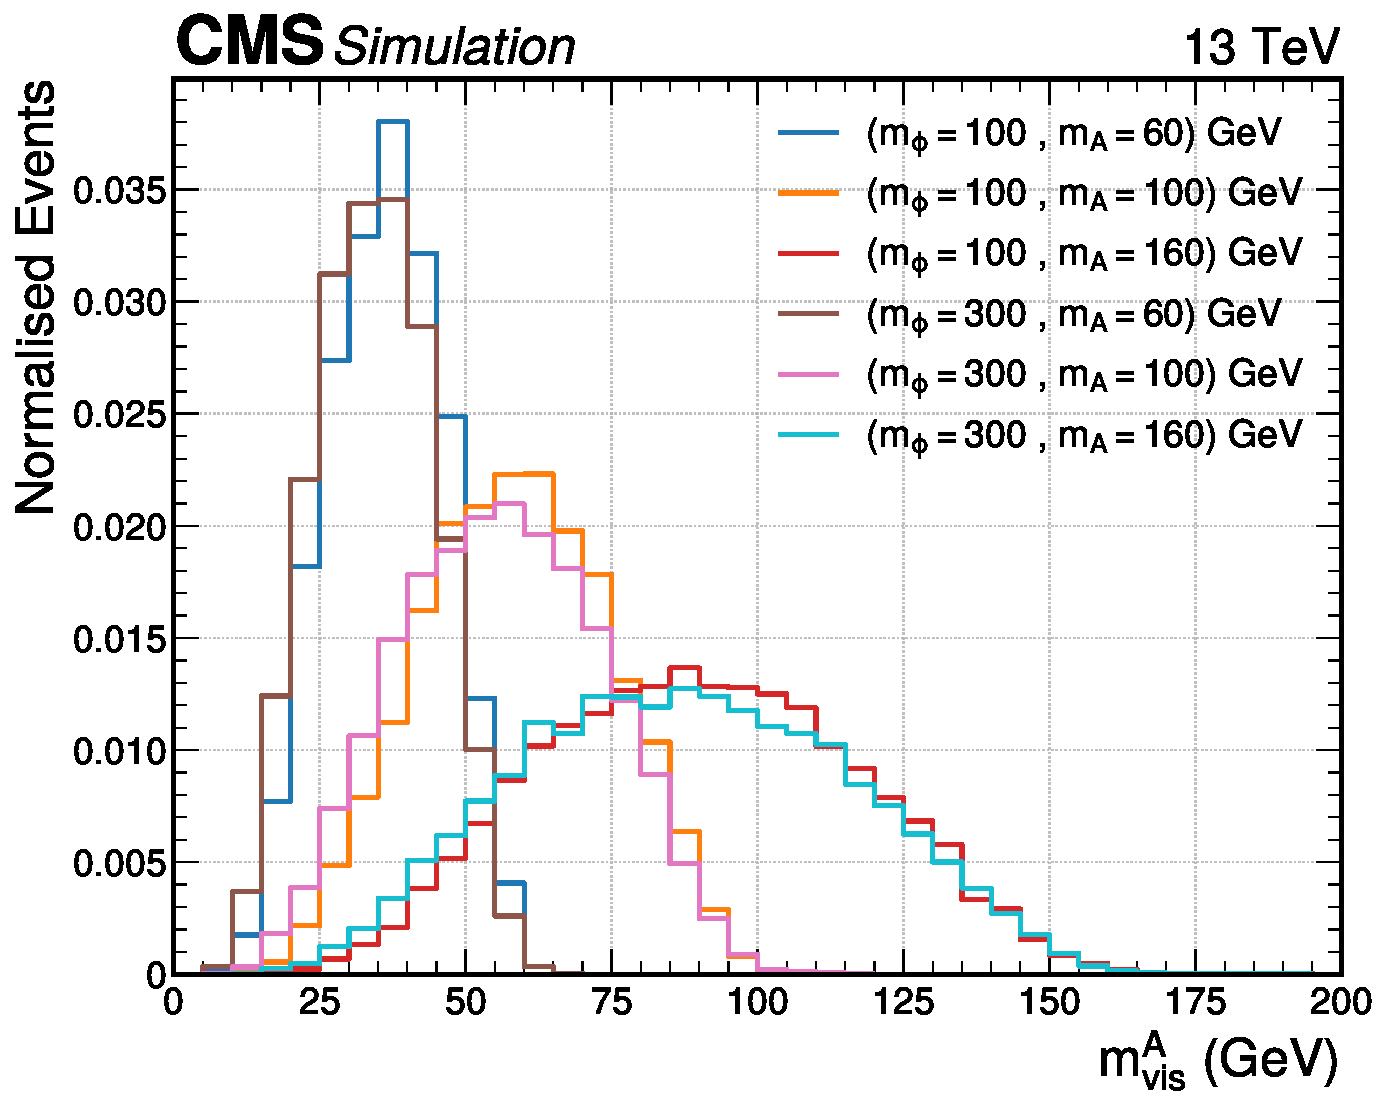
\includegraphics[width=\textwidth]{Figures/Chapter6/mvis_A.pdf}
            \caption{}
        \end{subfigure}
        \hfill
        \begin{subfigure}[b]{0.7\textwidth}
            \centering
            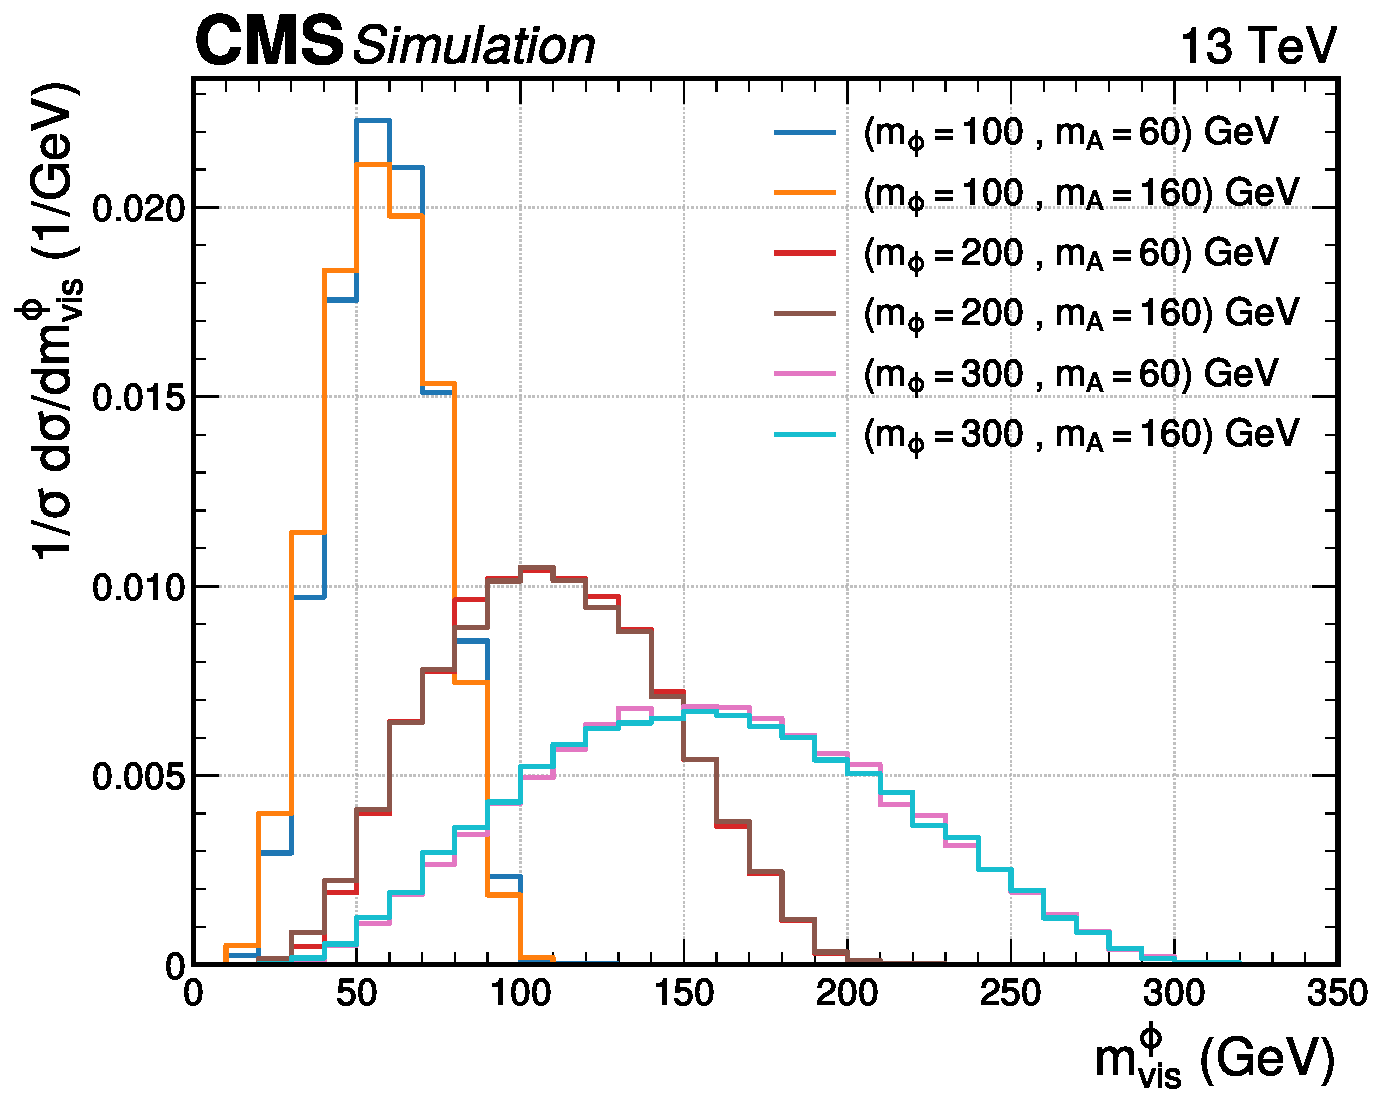
\includegraphics[width=\textwidth]{Figures/Chapter6/mvis_phi.pdf}
            \caption{}
        \end{subfigure}
    \caption[Generator-level visible mass distributions for different mass combinations of $\phi$ and A.]{Generator-level distributions of the visible di-$\PGt$ mass for selected combinations of $m_A$ and $m_\phi$. The visible mass is computed using only the decay products of the two $\PGt$ leptons, excluding neutrinos. Distributions are shown for scans over \textbf{(a)} $m_A$ and \textbf{(b)} $m_\phi$.}
    \label{Figure:Chapter6_GenVisDistributions}
\end{figure}

\subsection{Production cross sections and branching fractions}
\label{Section:Chapter6_production_xs_bf}
The production cross section is computed at \ac{NLO} in \ac{QCD} and is independent of $\tan\beta$ within the alignment limit. However, it varies significantly across the mass plane, ranging from approximately $650~\unit{fb}$ at $(m_\phi, m_A) = (100, 60)~\GeV$ to $10~\unit{fb}$ at $(300, 160)~\GeV$. Figure~\ref{Figure:Chapter6_ProductionXS} shows the cross section as a function of the two mass parameters under the alignment scenario. Outside this limit, the cross section acquires dependence on the scalar mixing angle:

\begin{itemize}
    \item It scales with $\sin^2(\beta - \alpha)$ when $\phi \equiv H$ ($m_\phi > 125~\GeV$),
    \item It scales with $\cos^2(\beta - \alpha)$ when $\phi \equiv h$ ($m_\phi \leq 125~\GeV$).
\end{itemize}

\begin{figure}[!htbp]
  \centering
  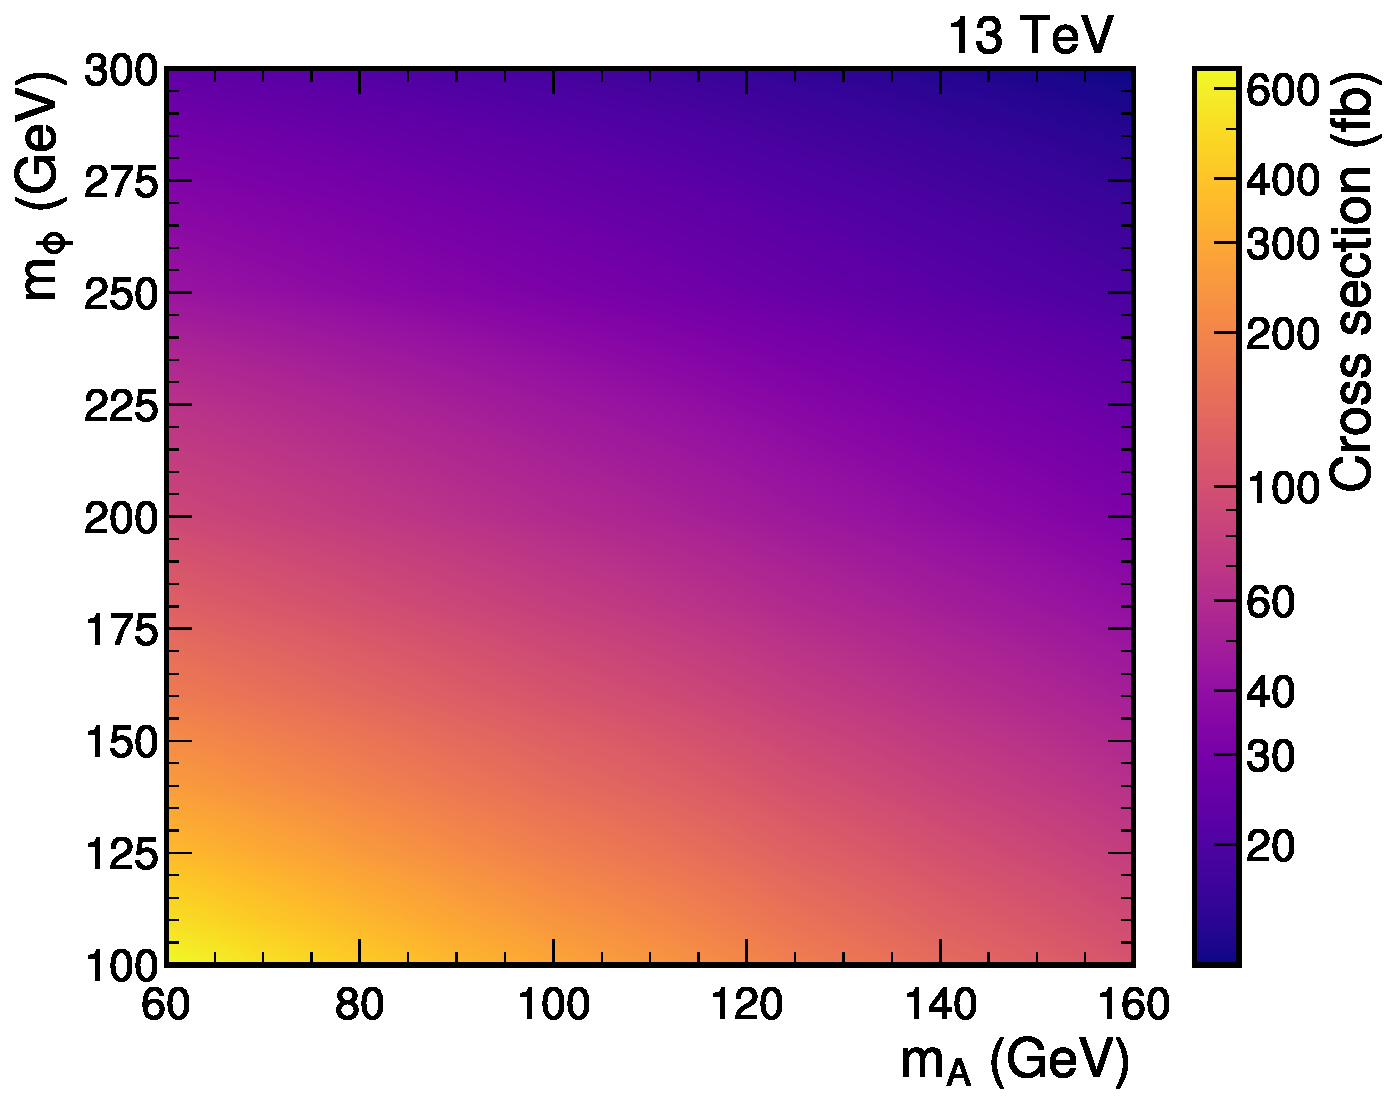
\includegraphics[width=0.7\textwidth]{Figures/Chapter6/Production_XS.pdf}
    \caption[Production cross sections for $Z^* \to \phi A$ in the alignment limit.]{Production cross sections for $Z^* \to \phi A$ in the alignment limit at \ac{NLO}, shown as a function of $m_\phi$ and $m_A$. The values are interpolated over a grid of simulated mass combinations.}
  \label{Figure:Chapter6_ProductionXS}
\end{figure}

The decay branching fractions of $\phi$ and $A$ into $\PGt^+\PGt^-$ are computed using \textsc{2HDECAY}~\cite{2HDECAY}, a dedicated tool for \ac{2HDM} decay widths and branching fractions. In the alignment limit, the $\PGt^+\PGt^-$ branching ratio of $A$ is close to unity for $\tan\beta \gtrsim 2$, but falls sharply at lower values, where hadronic decays such as $A \to b\bar{b}$ become dominant. A similar pattern holds for $\phi \to \PGt^+\PGt^-$, except when the mass difference $m_\phi - m_A$ exceeds $m_Z$. In this case, the decay $\phi \to ZA$ becomes kinematically accessible and can significantly suppress the ditau branching fraction, even at large $\tan\beta$. These features are illustrated in Fig.~\ref{Figure:Chapter6_BranchingFractions}, which shows representative branching fraction maps for selected mass configurations. 

\begin{figure}[!htbp]
        \centering
        % First row
        \begin{subfigure}[b]{0.49\textwidth}
            \centering
            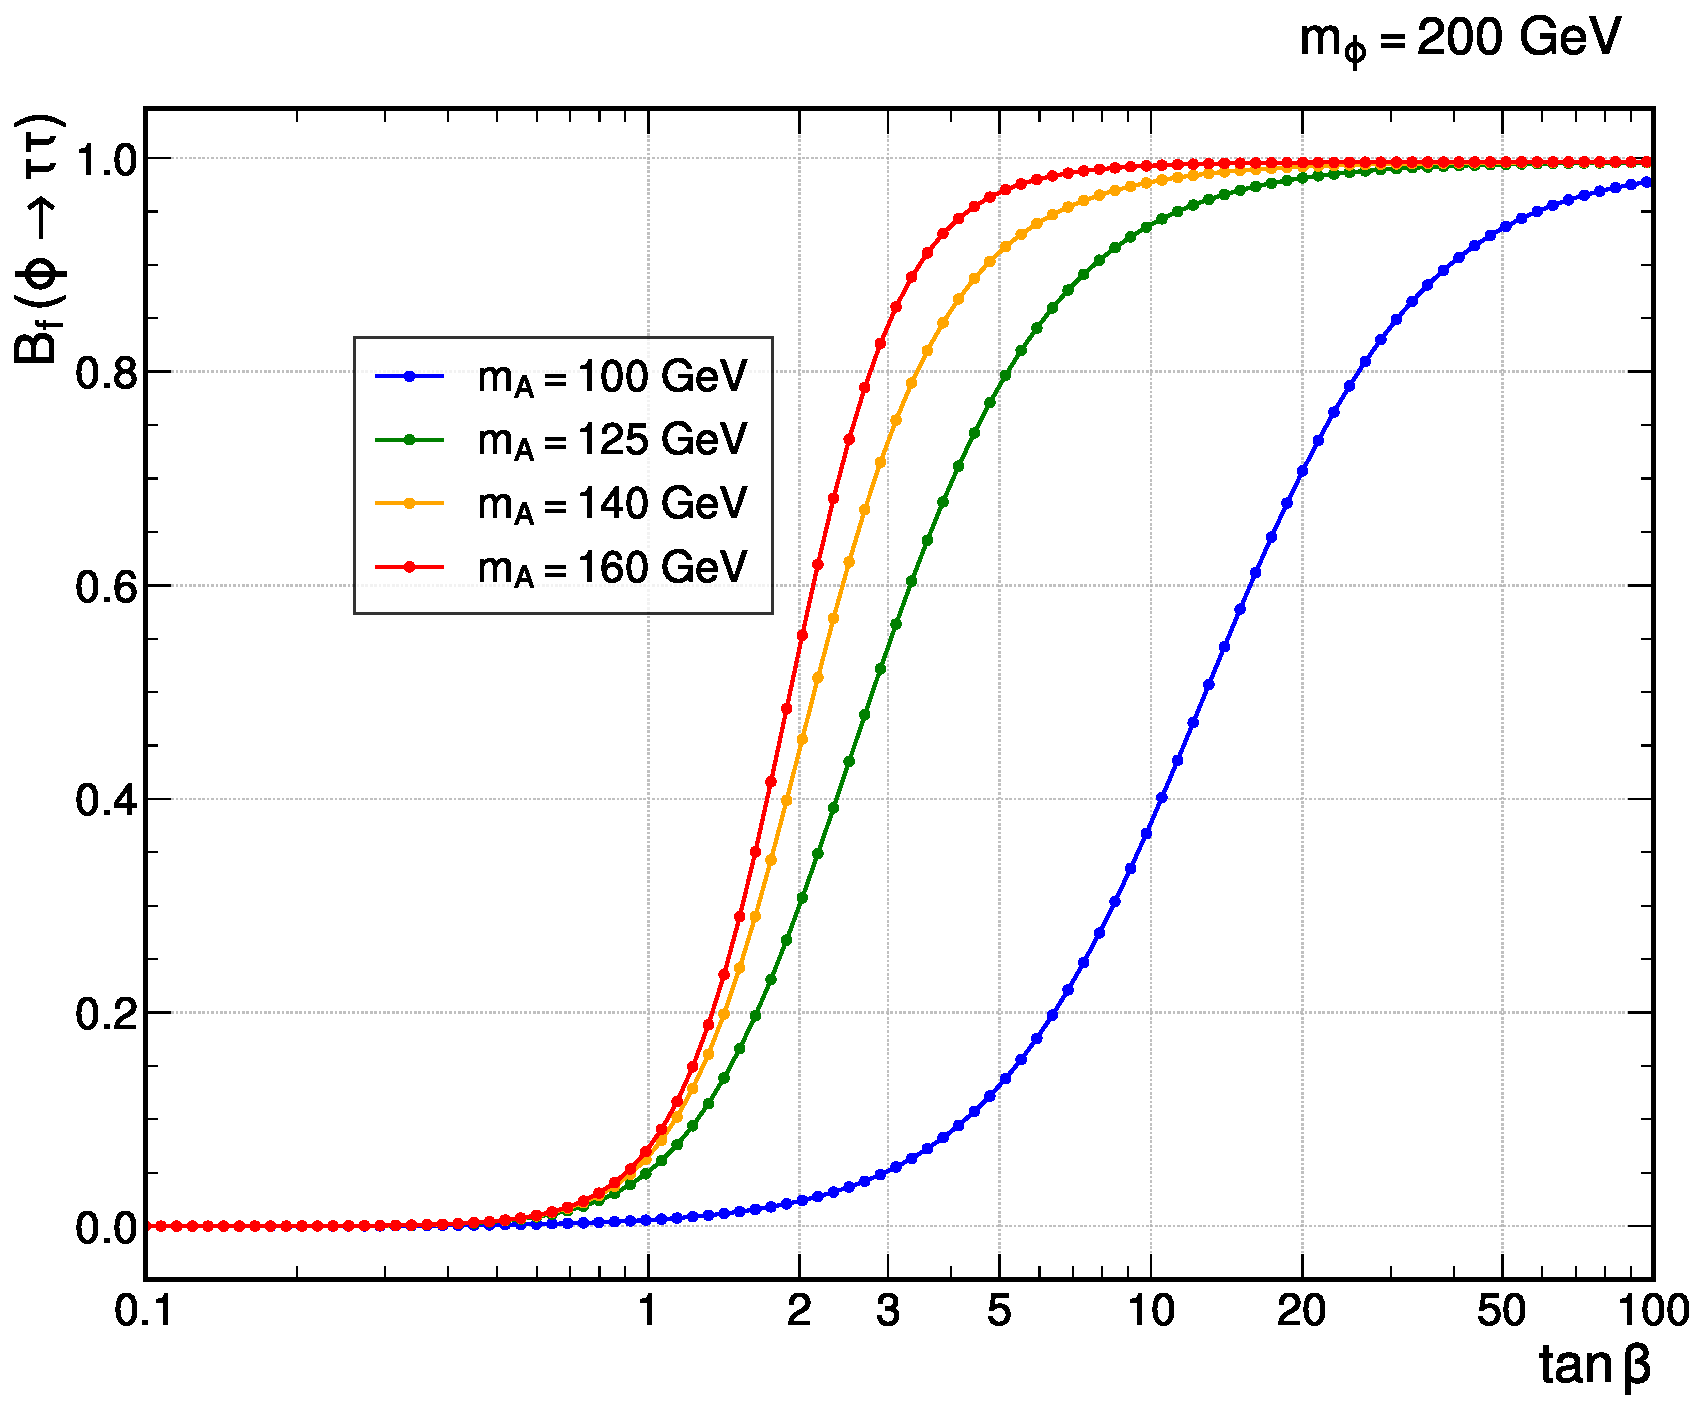
\includegraphics[width=\textwidth]{Figures/Chapter6/Phi_BR.pdf}
            \caption{}
        \end{subfigure}
        \begin{subfigure}[b]{0.49\textwidth}
            \centering
            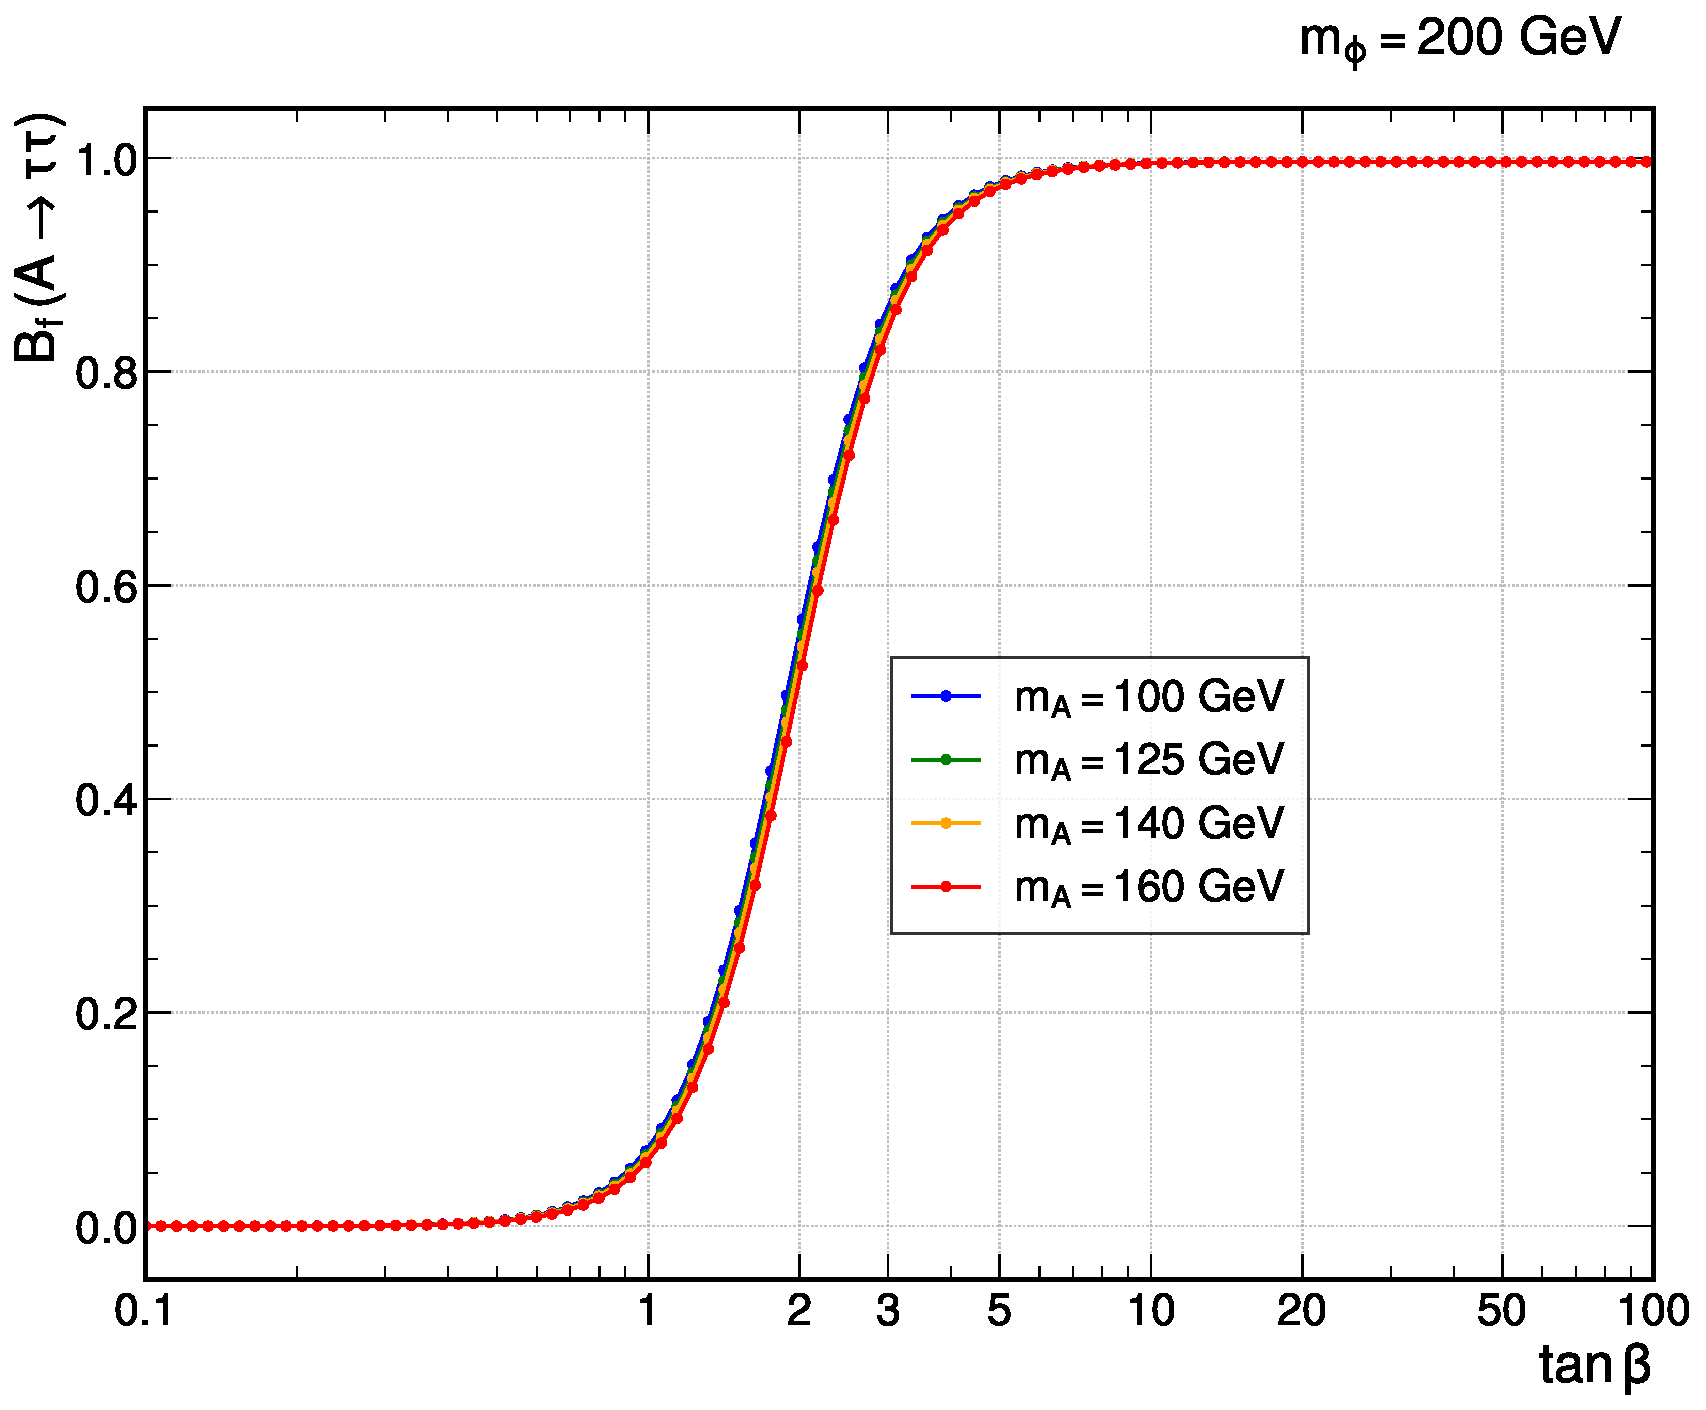
\includegraphics[width=\textwidth]{Figures/Chapter6/A_BR.pdf}
            \caption{}
        \end{subfigure}
    \caption[Branching fractions of $\phi$ and $A$ to $\PGt^+\PGt^-$ for selected mass combinations.]{Branching fractions of \textbf{(a)} $\phi \to \PGt^+\PGt^-$ and \textbf{(b)} $A \to \PGt^+\PGt^-$ as a function of $m_\phi$ and $m_A$, computed using \textsc{2HDECAY} in the alignment limit.}
    \label{Figure:Chapter6_BranchingFractions}
\end{figure}

\section{Event selection strategy}
\label{sec:ObjectAndEventSelections}

This analysis targets the process $Z^* \to \phi A \to 4\PGt$, where the four $\PGt$ leptons can give rise to a variety of final states depending on their \acp{DM}. The relative branching fractions of the most frequent final states are illustrated in Fig.~\ref{Figure:Chapter6_4tau_decayModes_BF}. Channels with at least two hadronically decaying $\PGt$ leptons ($\PGt_h$) dominate, accounting for 87.1\% of the total branching fraction, and therefore constitute the primary focus of the analysis.

\begin{figure}[!htbp]
  \centering
  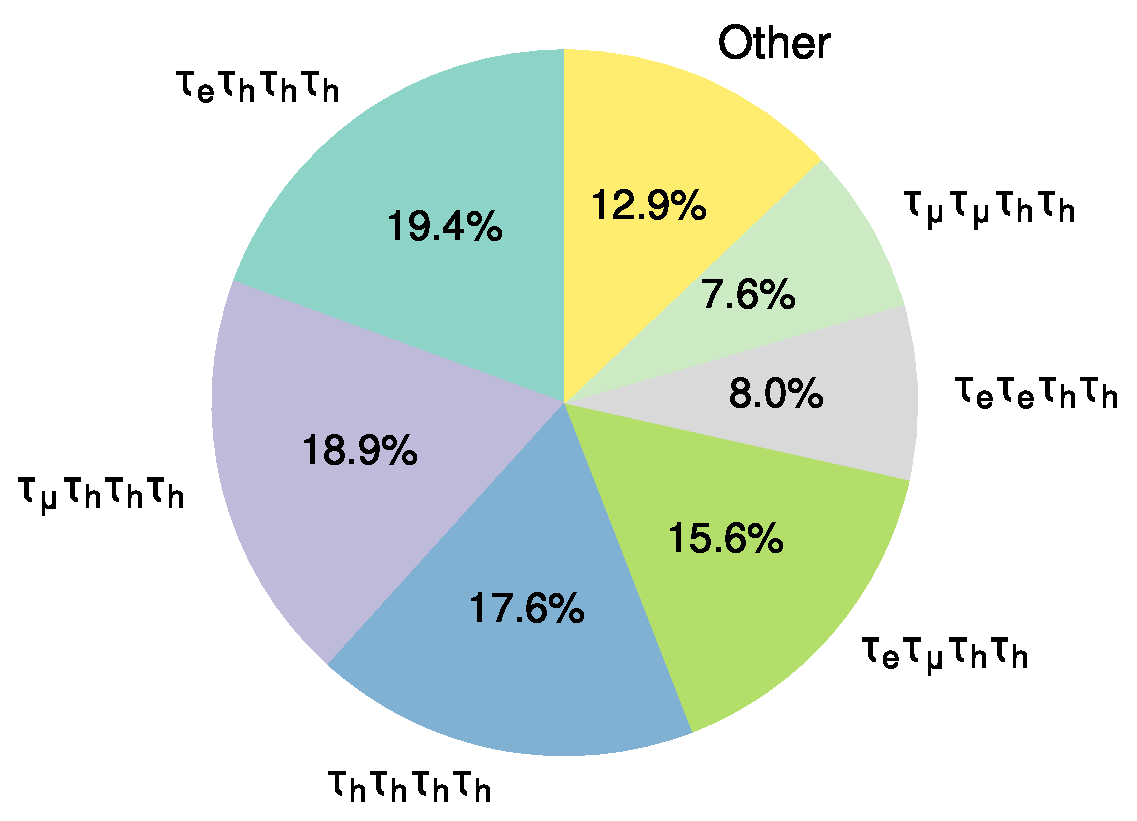
\includegraphics[width=0.8\textwidth]{Figures/Chapter6/pie_BF.pdf}
    \caption[Branching fractions of the dominant four-tau decay modes.]
    {Branching fractions of the most frequent four-tau final states, constructed by enumerating all combinations of tau decays.}
  \label{Figure:Chapter6_4tau_decayModes_BF}
\end{figure}

% \begin{table}[!htbp]
% \centering
% \renewcommand{\arraystretch}{1.5} % Increase row height
% \setlength{\tabcolsep}{12pt} % Increase column width
% \arrayrulecolor{black} % Ensure outer border is black
% \begin{tabular}{cc}
% \hline
% Decay Mode                  & Branching Fraction {[}\%{]} \\ \hline 
% $\PGt_e \PGt_e \PGt_{\mu} \PGt_h$             & 4.3 \\ 
% \arrayrulecolor{lightgray} \hline
% $\PGt_e \PGt_{\mu} \PGt_{\mu} \PGt_h$                    & 4.2 \\ 
% \arrayrulecolor{lightgray} \hline
% $\PGt_e \PGt_e \PGt_{e} \PGt_h$                        & 1.5  \\ 
% \arrayrulecolor{lightgray} \hline
% $\PGt_{\mu} \PGt_{\mu} \PGt_{\mu} \PGt_h$                  & 1.4  \\ 
% \arrayrulecolor{lightgray} \hline
% $\PGt_e \PGt_e \PGt_{\mu} \PGt_{\mu}$             & 0.6  \\ 
% \arrayrulecolor{lightgray} \hline
% $\PGt_e \PGt_e \PGt_{e} \PGt_{\mu}$                     & 0.4  \\ 
% \arrayrulecolor{lightgray} \hline
% $\PGt_e \PGt_{\mu} \PGt_{\mu} \PGt_{\mu}$             & 0.4  \\ 
% \arrayrulecolor{lightgray} \hline
% $\PGt_e \PGt_e \PGt_{e} \PGt_e$                  & 0.1  \\ 
% \arrayrulecolor{lightgray} \hline
% $\PGt_{\mu} \PGt_{\mu} \PGt_{\mu} \PGt_{\mu}$                  & 0.1  \\ 
% \arrayrulecolor{black} \hline
% \end{tabular}
% \caption[Branching fractions of subdominant four-tau decay modes]{Branching fractions of subdominant four-tau final states, involving three or more leptonic $\PGt$ decays.}
% \label{Table:Chapter6_4tau_decayModes_BF_Other}
% \end{table}

To improve acceptance for events in which one $\PGt_h$ fails to be reconstructed, an orthogonal $\PGt_h\PGt_h\PGt_h$ channel is also included. This typically captures partially reconstructed $\PGt_h\PGt_h\PGt_h\PGt_h$ decays where one candidate fails the trigger or identification requirements, often due to high $p_\text{T}$ thresholds or the finite efficiency of the tagging algorithm. With this addition, the total number of sensitive channels amounts to seven. Additionally, a control region based on the fully leptonic $\PGt_{\mu} \PGt_{\mu} \PGt_{\mu} \PGt_{\mu}$ final state is used to constrain the modelling of backgrounds composed entirely of genuine leptons, as discussed in Section~\ref{Section:Chapter6_Background_Modelling}.

\subsection{Triggering}

Identifying events with these topologies presents a unique challenge, as no dedicated trigger exists. Instead, the selection strategy relies on a combination of standard single- and multi-object triggers that are sensitive to subsets of the final-state decay products. These include single-lepton (electron or muon), double-electron, double-muon, and double-tau triggers. Cross-triggers, such as those combining a lepton and a hadronic tau ($e+\tau_h$, $\mu+\tau_h$) or the electron–muon trigger, were also considered. However, they provided negligible gains in signal acceptance and so were excluded. Although single-$\tau_h$ triggers are also available, their high $p_\text{T}$ thresholds are too restrictive for the phase space relevant to this search. The triggers used in the analysis, along with the corresponding online $p_\text{T}$ thresholds for each data-taking year, are summarised in Table~\ref{Table:Chapter6_TriggerThresholdsExpanded}.

\begin{table}[!htbp]
\centering
\renewcommand{\arraystretch}{1.5}
\setlength{\tabcolsep}{12pt} % Increase column width
\begin{tabular}{|c|cc|cc|cc|}
\hline
\multirow{3}{*}{\text{Trigger}} 
& \multicolumn{6}{c|}{$p_\text{T}$ \text{Threshold (GeV)}} \\ \cline{2-7}
& \multicolumn{2}{c|}{\text{2016}} & \multicolumn{2}{c|}{\text{2017}} & \multicolumn{2}{c|}{\text{2018}} \\ \cline{2-7}
& \text{Obj$_1$} & \text{Obj$_2$} & \text{Obj$_1$} & \text{Obj$_2$} & \text{Obj$_1$} & \text{Obj$_2$} \\ \hline \hline
Single-Electron (e)                   & 26     & --     & 28     & --     & 33     & --     \\
\arrayrulecolor{lightgray} \hline
Single-Muon ($\mu$)                       & 23     & --     & 25     & --     & 25     & --     \\
\arrayrulecolor{lightgray} \hline
Double-Tau ($\PGt \PGt$)         & 40     & 40     & 40     & 40     & 40     & 40     \\
\arrayrulecolor{black} \hline
\end{tabular}
\caption{Table of minimum online $p_\text{T}$ thresholds for the triggers used in the analysis. Subcolumns refer to thresholds for the first and second trigger objects.}
\label{Table:Chapter6_TriggerThresholdsExpanded}
\end{table}

The trigger configuration applied to each channel is summarised in Table~\ref{Table:Chapter6_TriggersPerChannel}. A trigger is considered to have fired for a given event if any of the listed object combinations satisfy the corresponding online requirements. The logical OR operator ($\lor$) denotes the inclusive selection, corresponding to the union of all trigger paths associated with that channel.

\begin{table}[!htbp]
\centering
\renewcommand{\arraystretch}{1.5}
\setlength{\tabcolsep}{12pt}
\begin{tabular}{cc}
\hline
Channel & Trigger Configuration \\ \hline 

$\tau_h\tau_h\tau_h\tau_h$ &  
$\tau_1\tau_2 \mathbin{\lor} \tau_1\tau_3 \mathbin{\lor} \tau_1\tau_4 \mathbin{\lor} \tau_2\tau_3 \mathbin{\lor} \tau_2\tau_4 \mathbin{\lor} \tau_3\tau_4$ \\ 
\arrayrulecolor{lightgray} \hline

$\tau_h\tau_h\tau_h$ &
$\tau_1\tau_2 \mathbin{\lor} \tau_1\tau_3 \mathbin{\lor} \tau_2\tau_3$ \\
\arrayrulecolor{lightgray} \hline

$\tau_e\tau_h\tau_h\tau_h$ &
$e_1 \mathbin{\lor} \tau_2\tau_3 \mathbin{\lor} \tau_2\tau_4 \mathbin{\lor} \tau_3\tau_4$ \\
\arrayrulecolor{lightgray} \hline

$\tau_\mu\tau_h\tau_h\tau_h$ &
$\mu_1 \mathbin{\lor} \tau_2\tau_3 \mathbin{\lor} \tau_2\tau_4 \mathbin{\lor} \tau_3\tau_4$ \\
\arrayrulecolor{lightgray} \hline

$\tau_e\tau_e\tau_h\tau_h$ &
$e_1 \mathbin{\lor} e_2 \mathbin{\lor} \tau_3\tau_4$ \\
\arrayrulecolor{lightgray} \hline

$\tau_\mu\tau_\mu\tau_h\tau_h$ &
$\mu_1 \mathbin{\lor} \mu_2 \mathbin{\lor} \tau_3\tau_4$ \\
\arrayrulecolor{lightgray} \hline

$\tau_e\tau_\mu\tau_h\tau_h$ &
$e_1 \mathbin{\lor} \mu_1 \mathbin{\lor} \tau_3\tau_4$ \\
\arrayrulecolor{lightgray} \hline

$\tau_\mu \tau_\mu \tau_\mu \tau_\mu$ &
$\mu_1 \mathbin{\lor} \mu_2 \mathbin{\lor} \mu_3 \mathbin{\lor} \mu_4$ \\
\arrayrulecolor{black} \hline

\end{tabular}
\caption[Trigger configuration used for each four-tau final state.]{Trigger configuration used for each four-tau final state. The labels $e_i$, $\mu_i$, and $\tau_i$ denote individual trigger objects corresponding to electrons, muons, and hadronic taus, respectively, with index $i$ indicating the ordering of candidates in the event.}
\label{Table:Chapter6_TriggersPerChannel}
\end{table}

\subsection{Offline object selections}
\label{Section:Chapter6_ObjectSelection}

Offline selection criteria are applied to reconstructed electrons, muons, and $\PGt_h$candidates, as introduced in Chapter~\ref{Section:Chapter4}. These selections suppress backgrounds from nonprompt and misidentified particles while maintaining high signal efficiency. To ensure consistency with the \ac{PV} and reduce contamination from \ac{PU}, all selected objects are required to originate from the \ac{PV}. This is enforced through cuts on transverse and longitudinal impact parameters: $|d_{xy}| < 0.045\unit{cm}$ and $|d_z| < 0.2\unit{cm}$ for electrons and muons, and $|d_z| < 0.2\unit{cm}$ for $\PGt_h$ candidates.

Electrons and muons are additionally required to be isolated from nearby hadronic activity. The relative isolation, defined in Chapter~\ref{Section:Chapter4} (Equations~\ref{Equation:Chapter4_PFIso_Electron} and~\ref{Equation:Chapter4_PFIso_Muon}), is required to satisfy $I^{e/\mu}_\text{PF} < 0.15$. No explicit isolation cut is applied to hadronic tau candidates, as this information is embedded in the DeepTau discriminators.

Identification criteria follow those detailed in Sections~\ref{Section:Electron_Identification},~\ref{Section:Muon_Identification}, and~\ref{Section:Chapter4_Taus}. Electrons are selected using a BDT-based discriminator targeting 90\% efficiency, with isolation variables excluded from the training. Muons are required to pass the cut-based medium \ac{WP}. For $\PGt_h$ candidates, a looser identification is applied to retain adequate signal yields. Candidates must pass the Loose \ac{WP} of the $D_{\text{jet}}$ discriminator, along with misidentified-lepton rejection cuts: VVLoose for $D_e$ and VLoose for $D_\mu$. 

To ensure consistency between trigger and offline reconstruction, selected objects must match the corresponding trigger-level objects within a cone of $\Delta R < 0.5$. The number of required matches depends on the trigger configuration for each channel, as outlined in Table~\ref{Table:Chapter6_TriggersPerChannel}. For channels using double-object triggers (\eg $\tauh\tauh\tauh\tauh$), any two $\tauh$ must be matched. In channels triggered by single leptons (\eg, $\tau_e\tauh\tauh\tauh$), only one matched object is required, depending on the path fired. Stricter $p_T$ thresholds are applied to trigger-matched objects to ensure operation in the plateau of the trigger efficiency turn-on curve. These are $+1\GeV$ for electrons and muons, and $+5\GeV$ for hadronic tau candidates. Unmatched objects are subject to looser baseline thresholds. This conditional strategy maximises acceptance while preserving accurate modelling of trigger efficiencies.

A full summary of the offline selection criteria is given in Table~\ref{Table:Chapter6_ObjectSelectionSummary}.

{
\setlength{\arrayrulewidth}{1pt}

% Move the caption BEFORE the table
\begin{table}[!htbp]
\centering
\caption[Summary of baseline object selection criteria]{
Summary of baseline selection criteria applied to reconstructed electrons, muons, and hadronically decaying taus. Trigger-matched $p_T$ thresholds are defined relative to those in Table~\ref{Table:Chapter6_TriggerThresholdsExpanded}.
}
\label{Table:Chapter6_ObjectSelectionSummary}

\renewcommand{\arraystretch}{1.5}
\setlength{\tabcolsep}{12pt}
\arrayrulecolor{black}

\begin{tabular}{cccc}
\hline
Criteria & Electron & Muon & Hadronic Tau \\
\hline

$p_\text{T}$  & > $10\GeV$ & > $10\GeV$ & > $20\GeV$\\ 
\arrayrulecolor{lightgray} \hline

$p_\text{T}^{\text{Trigger}}$ & \multicolumn{3}{c}{$> \text{Table~\ref{Table:Chapter6_TriggerThresholdsExpanded}} + [1,\,1,\,5]$} \\
\arrayrulecolor{lightgray} \hline

$|\eta|$ & < $2.5$ & < $2.4$ & < $2.3$/$2.1$\hyperlink{DoubleTauTrigger-EtaCut}{$^1$} \\
\arrayrulecolor{lightgray} \hline

$|d_{xy}|$ & < $0.045\unit{cm}$ & < $0.045\unit{cm}$ & -- \\
\arrayrulecolor{lightgray} \hline

$|d_z|$ & < $0.2\unit{cm}$ & < $0.2\unit{cm}$ & < $0.2\unit{cm}$ \\
\arrayrulecolor{lightgray} \hline

Isolation & $I^e_\text{PF}$ < 0.15 & $I^\mu_\text{PF}$ < 0.15 & -- \\
\arrayrulecolor{lightgray} \hline

Identification
& \makecell{\ac{MVA} w/o isolation\\(90\% \ac{WP})}
& Medium ID
& \makecell{
\normalfont\footnotesize$D_{\text{jet}} \geq$ Loose\hyperlink{Alternative-FFcut}{$^2$} \\
\normalfont\footnotesize$D_{e} \geq$ VVLoose \\
\normalfont\footnotesize$D_{\mu} \geq$ VLoose
} \\
\arrayrulecolor{black} \hline
\end{tabular}
\vspace{0.5em}
\begin{minipage}{0.95\linewidth}
\raggedright
\footnotesize
\hypertarget{DoubleTauTrigger-EtaCut}{}$^{1}$\,$|\eta| < 2.1$ is required for $\tauh$ candidates matched to trigger objects, reflecting the online trigger acceptance region. \\

\vspace{0.5em}

\hypertarget{Alternative-FFcut}{}$^{2}$\,The Loose \ac{WP} is referred to as the \texttt{Nominal} tau identification in the fake factor method (see Section~\ref{Section:Chapter6_JetToTauBackground}). An \texttt{Alternative} selection, defined as $D_{\text{jet}} > 0.1$, is used to construct control regions.

\end{minipage}

\end{table}
}

\subsection{Event-level selections}

Beyond object-level requirements, additional selection criteria are imposed at the event level to enhance signal purity and ensure statistical orthogonality between channels. In channels containing light leptons, $b$-jet vetoes are applied to suppress $\ttbar$ background. Charge requirements are used to enforce consistency with the signal topology, reflecting both the electrically neutral nature of the parent bosons ($Z^* \to \phi A$). In contrast, a total charge of $\pm1$ is permitted in the $\tauh\tauh\tauh$ channel to account for one potentially unreconstructed tau. Additional constraints on the number of reconstructed objects are also applied, depending on the channel. The full set of event-level selection criteria for each channel is summarised in Table~\ref{Table:Chapter6_Event_Channel_Selections}.

{
\setlength{\arrayrulewidth}{1pt}

% Move the caption BEFORE the table
\begin{table}[!htbp]
\caption[Event-level selection requirements applied to each four-tau final state.]{
Event-level selection criteria applied to each four-tau final state. The table specifies the required number of electrons, muons, hadronic taus, and $b$-tagged jets, as well as the total charge requirement for the selected objects.}
\label{Table:Chapter6_Event_Channel_Selections}
\centering
\renewcommand{\arraystretch}{1.5}
\setlength{\tabcolsep}{12pt}
\arrayrulecolor{black}

\begin{tabular}{cccccc}
\hline
Channel & $\mathcal{N}_\text{electrons}$ & $\mathcal{N}_\text{muons}$ & $\mathcal{N}_{\PGt_h}$ & $\mathcal{N}_{b_\text{jets}}$\hyperlink{b-jet_selections}{$^1$} & $\sum\text{q}$\\
\hline

$\tau_h\tau_h\tau_h\tau_h$ &  0 & 0 & $\geq 4$ & $\geq 0$ & 0\\
\arrayrulecolor{lightgray} \hline

$\tau_h\tau_h\tau_h$ & 0 & 0 & 3 & $\geq 0$ & $\pm 1$\\
\arrayrulecolor{lightgray} \hline

$\tau_e\tau_h\tau_h\tau_h$ & 1 & 0 & $\geq3$ & $0$  & 0 \\
\arrayrulecolor{lightgray} \hline

$\tau_\mu\tau_h\tau_h\tau_h$ & 0 & 1 & $\geq 3$ & $0$ & 0 \\
\arrayrulecolor{lightgray} \hline

$\tau_e\tau_e\tau_h\tau_h$ & 2 & 0 & $\geq 2$ & $0$ & 0\\
\arrayrulecolor{lightgray} \hline

$\tau_\mu\tau_\mu\tau_h\tau_h$ & 0 & 2 & $\geq 2$ & $0$ & 0 \\
\arrayrulecolor{lightgray} \hline

$\tau_e\tau_\mu\tau_h\tau_h$ & 1 & 1 & $\geq 2$ & $0$ & 0 \\
\arrayrulecolor{black} \hline
\end{tabular}
\vspace{0.5em}
\begin{minipage}{0.95\linewidth}
\raggedright
\footnotesize\hypertarget{b-jet_selections}{}$^{1}$\,Jets are required to pass the $b$-tagging criteria defined in Chapter~\ref{Section:Chapter4}, have $p_T > 30\GeV$, $|\eta| < 4.7$ and not overlap with any selected electron, muon or $\tauh$ candidates within $\Delta R < 0.5$.
\end{minipage}
\end{table}
}


\section{Object and event corrections}

Simulated events are subject to various imperfections, leading to discrepancies with data. These originate from several sources, including the limited precision of \ac{MC} event generators, approximations in detector simulation, and differences in reconstruction performance. In particular, discrepancies may arise between simulated and real objects in their probability of satisfying selection criteria such as ID, isolation, or trigger requirements. Mismatches in detector response can also cause systematic shifts in reconstructed object energies.

To address these effects, a series of corrections, referred to as \acp{SF}, are applied to simulated events to improve agreement with data. These include object-level adjustments, such as energy scale and resolution corrections, as well as event-level weights such as \ac{PU} corrections.

Wherever possible, corrections provided centrally by the \ac{CMS} collaboration are used. However, for analysis-specific selections or nonstandard trigger paths, dedicated corrections are derived to ensure consistency with the data-taking conditions and selection strategy employed. The remainder of this section summarises the key corrections applied to simulated events in this analysis.

\subsection{Pileup reweighting}

Accurate modelling of \ac{PU} interactions is essential to reflect the conditions observed during data taking. In simulation, the \ac{PU} profile, defined as the distribution of the mean number of interactions per bunch crossing, is constructed based on the expected instantaneous luminosity for each year. 

In \ac{CMS} simulation, the \ac{PU} conditions under which each event is generated are characterised by a ``true'' mean number of additional interactions, denoted by $\mu^{\text{PU}}$. This value is randomly drawn from the simulated \ac{PU} profile. The actual number of \ac{PU} interactions, including both in-time and out-of-time contributions\footnote{In-time \ac{PU} refers to additional pp interactions occurring in the same bunch crossing. Conversely, out-of-time \ac{PU} refers to energy deposits in preceding or following bunch crossing.}, is then sampled from a Poisson distribution with this mean. However, the simulated \ac{PU} profile may differ from the true distribution observed in data. To account for this, a per-event weight is applied to reweight the simulation such that its \ac{PU} distribution matches that of the data. Figure~\ref{Figure:Chapter6_PU_Profiles} shows a comparison of the \ac{PU} distributions in data and simulation during the \ac{CMS} Run 2 data-taking period, illustrating the need for reweighting.

\begin{figure}[!htbp]
\centering
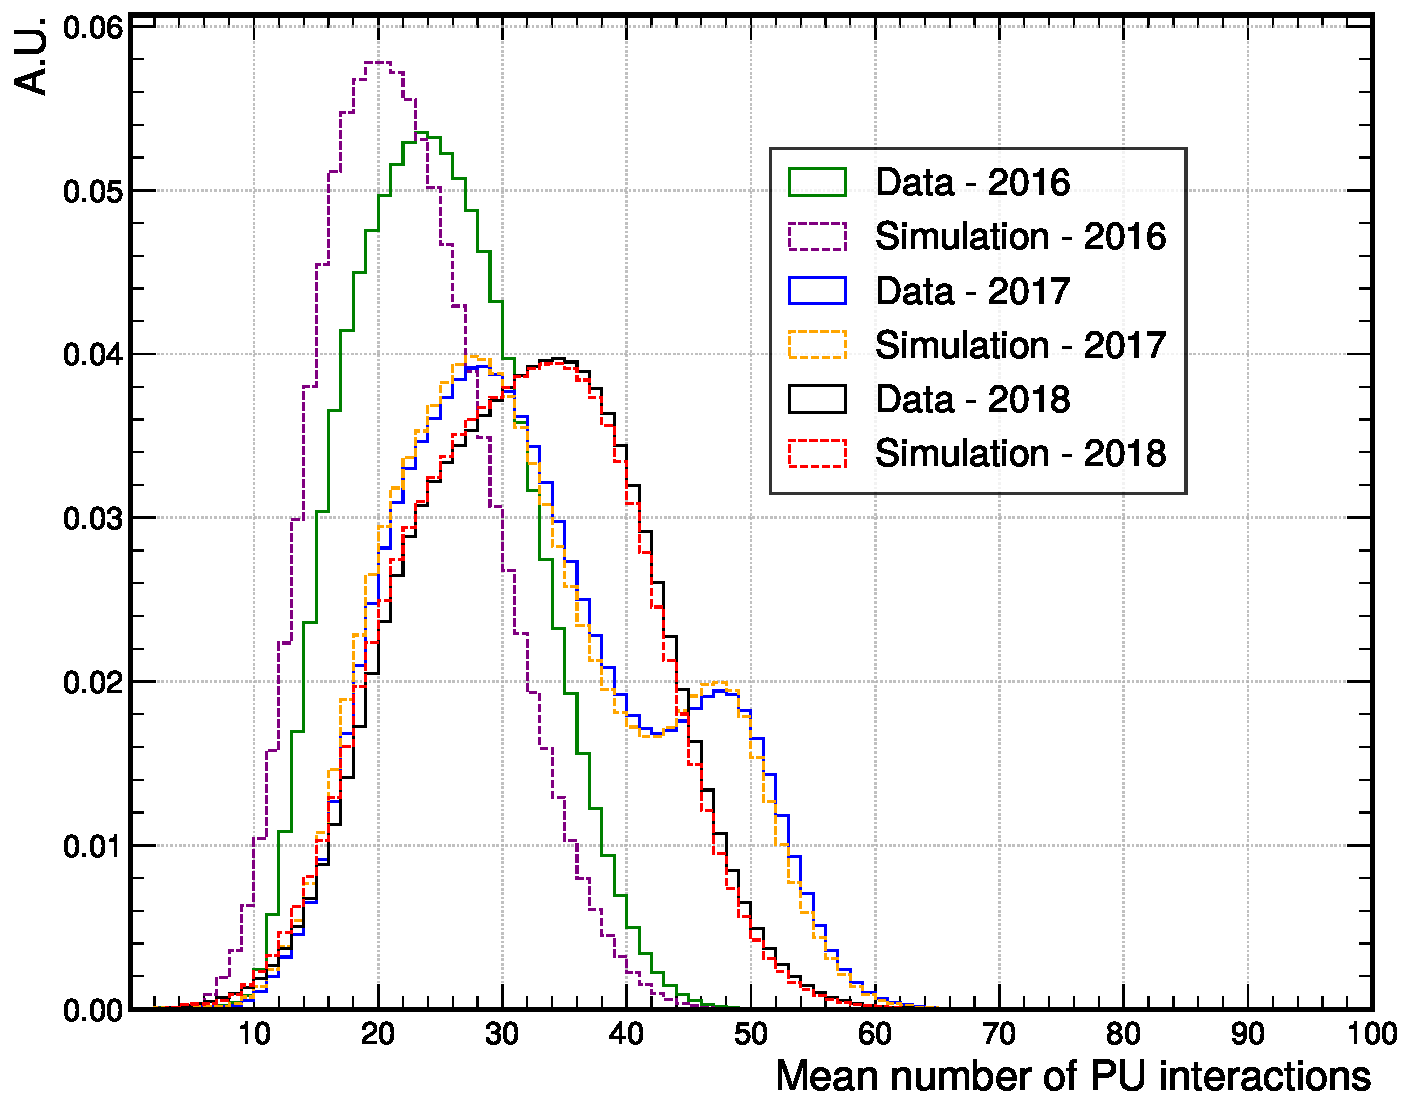
\includegraphics[width=0.8\textwidth]{Figures/Chapter6/PU_Profile.pdf}
\caption{Comparison of the distributions of the mean number of proton-proton interactions per bunch crossing between data and simulation in CMS Run 2.}
\label{Figure:Chapter6_PU_Profiles}
\end{figure}

\subsection{Electrons and Muons}
\label{Section:Chapter6_LightLepton_Corrections}

Although simulated light leptons are reconstructed using algorithms designed to replicate those used in data, residual differences remain and must be corrected. These corrections address different components of the reconstruction and selection process, including tracking, identification, isolation, and triggering.

Tracking corrections are derived centrally by the \ac{CMS} collaboration and applied directly. However, all other electron and muon corrections are measured within this analysis using a dedicated implementation of the \textit{tag-and-probe} method~\cite{CMS_Muon_System_Performance,CMS_Muon_System_Performance_2}. This approach is necessary because the object selection criteria used in this analysis are not standard. Particularly, the impact parameter requirements on $d_{xy}$ and $d_z$, as summarised in Table~\ref{Table:Chapter6_ObjectSelectionSummary}, differ from those used in the official \ac{CMS} efficiency measurements.

The tag-and-probe technique is applied to leptons from $\PZ \rightarrow \ell^+\ell^-$ decays, which provide a clean and unbiased sample for assessing selection performance. Events are selected by requiring an opposite-charge, same-flavour lepton pair with invariant mass $m_{\ell\ell}$ between $65\GeV$ and $115\GeV$, enhancing the $\PZ$ boson purity. One lepton, the \textit{tag}, is required to pass tight identification, isolation, and single-lepton trigger criteria, ensuring it does not bias the measurement of the second lepton, the \textit{probe}. To maximise statistical precision, if both leptons pass the tag requirements, each can in turn serve as the probe. Efficiencies are measured in bins of probe $p_{\mathrm{T}}$ and $\eta$ to account for detector and kinematic variations. The probe requirements for each selection stage are:

\begin{enumerate}[label=(\roman*)]
    \item Identification: Only requires identification
    \item Isolation: Requires identification, but not trigger.
    \item Trigger: Requires both identification and isolation.
\end{enumerate}

In each ($p_{\mathrm{T}}$, $\eta$) bin, events are split into ``pass'' and ``fail'' categories depending on whether the probe satisfies the selection under study. A simultaneous fit to the dilepton invariant mass distribution in both categories is used to extract the number of $\PZ \rightarrow \ell^+\ell^-$ signal events, accounting for residual background contamination. The signal is modelled with a sum of Voigtian functions, using the $\PZ$ boson’s natural width for the Breit-Wigner component. Backgrounds are modelled using:

\begin{itemize}
    \item A decaying exponential for the isolation and trigger fits.
    \item An error function transitioning to a decaying exponential for the identification fits, where background contamination is larger.
\end{itemize}

The efficiency is then extracted as:

\begin{equation_pad}
    \epsilon = \frac{N_{\text{pass}}}{N_{\text{pass}} + N_{\text{fail}}}
\end{equation_pad}

where $N_{\text{pass}}$ and $N_{\text{fail}}$ are the fitted $Z \rightarrow \ell^+\ell^-$ yields in each category. Figure~\ref{Figure:Chapter6-TagAndProbeFits_Nominal} shows an example fit for muons in a representative $\eta$ bin.

\begin{figure}[!htbp]
\centering
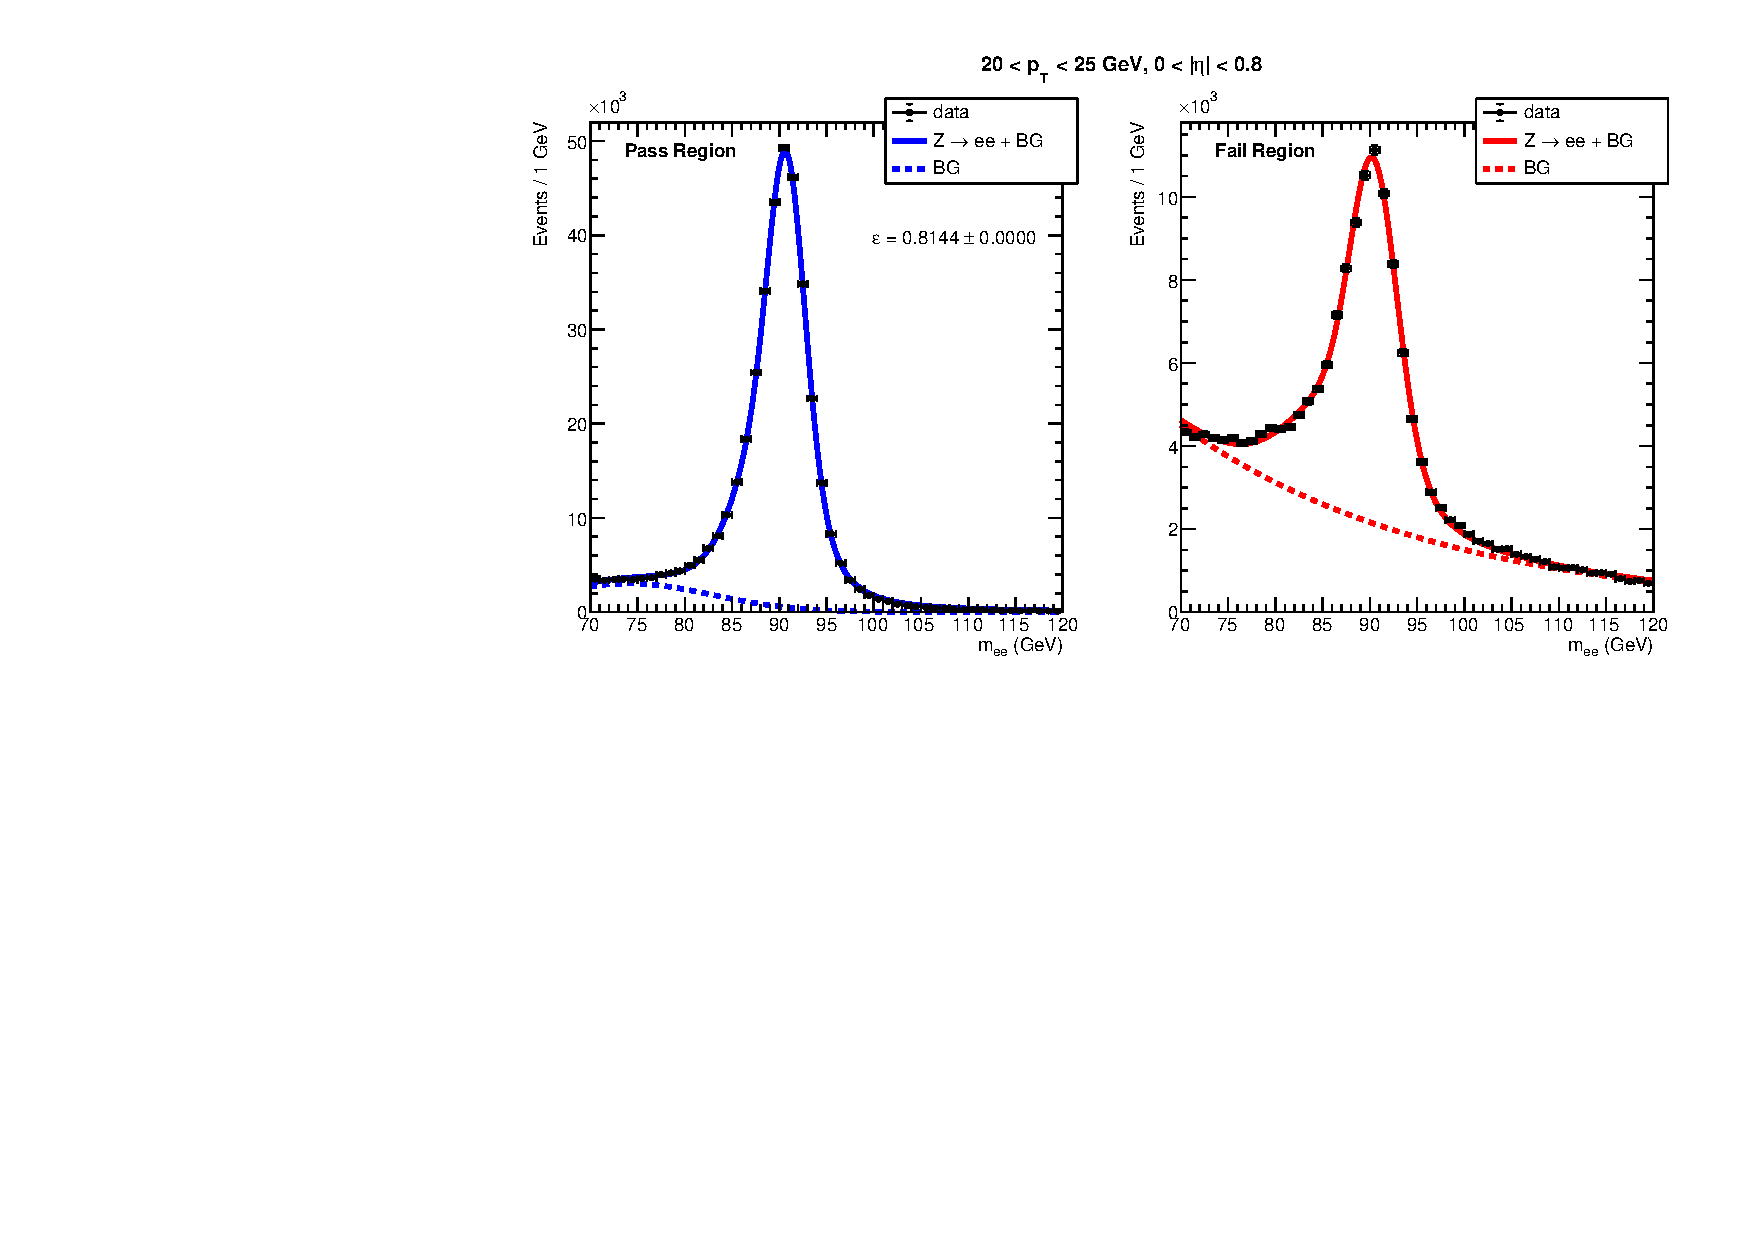
\includegraphics[width=\textwidth]{Figures/Chapter6/data_id_pt_20_to_25_eta_0.0_to_0.8_tpzee_nominal.pdf}
\caption{Example of the tag-and-probe fit used to extract electron identification efficiency in data. This plot corresponds to the $p_{\mathrm{T}}$ bin $20–25\GeV$ and the $|\eta|$ region 0.0–0.8.}
\label{Figure:Chapter6-TagAndProbeFits_Nominal}
\end{figure}

Efficiency SFs are then computed as the ratio of data and simulation efficiencies:

\begin{equation_pad}
    \text{SF}(p_\text{T},\eta) = \frac{\epsilon_\text{data}(p_\text{T},\eta)}{\epsilon_\text{MC}(p_\text{T},\eta)}
\end{equation_pad}

where these SFs are applied per object, and the total event-level correction is given by the product of the SFs for all leptons in the event.

Systematic uncertainties are estimated by varying aspects of the tag-and-probe procedure. These variations include modifying the tag lepton $p_{\text{T}}$ threshold (e.g., from $25\GeV$ to $35\GeV$), using alternative signal models, and changing the background parameterisation. Figure~\ref{Figure:Chapter6-TagAndProbeFits_Alternative} shows a representative comparison between the nominal fit configuration and a variant with a tighter tag lepton requirement. The resulting differences in efficiency are propagated as systematic uncertainties on the SFs.

\begin{figure}[!htbp]
    \centering
    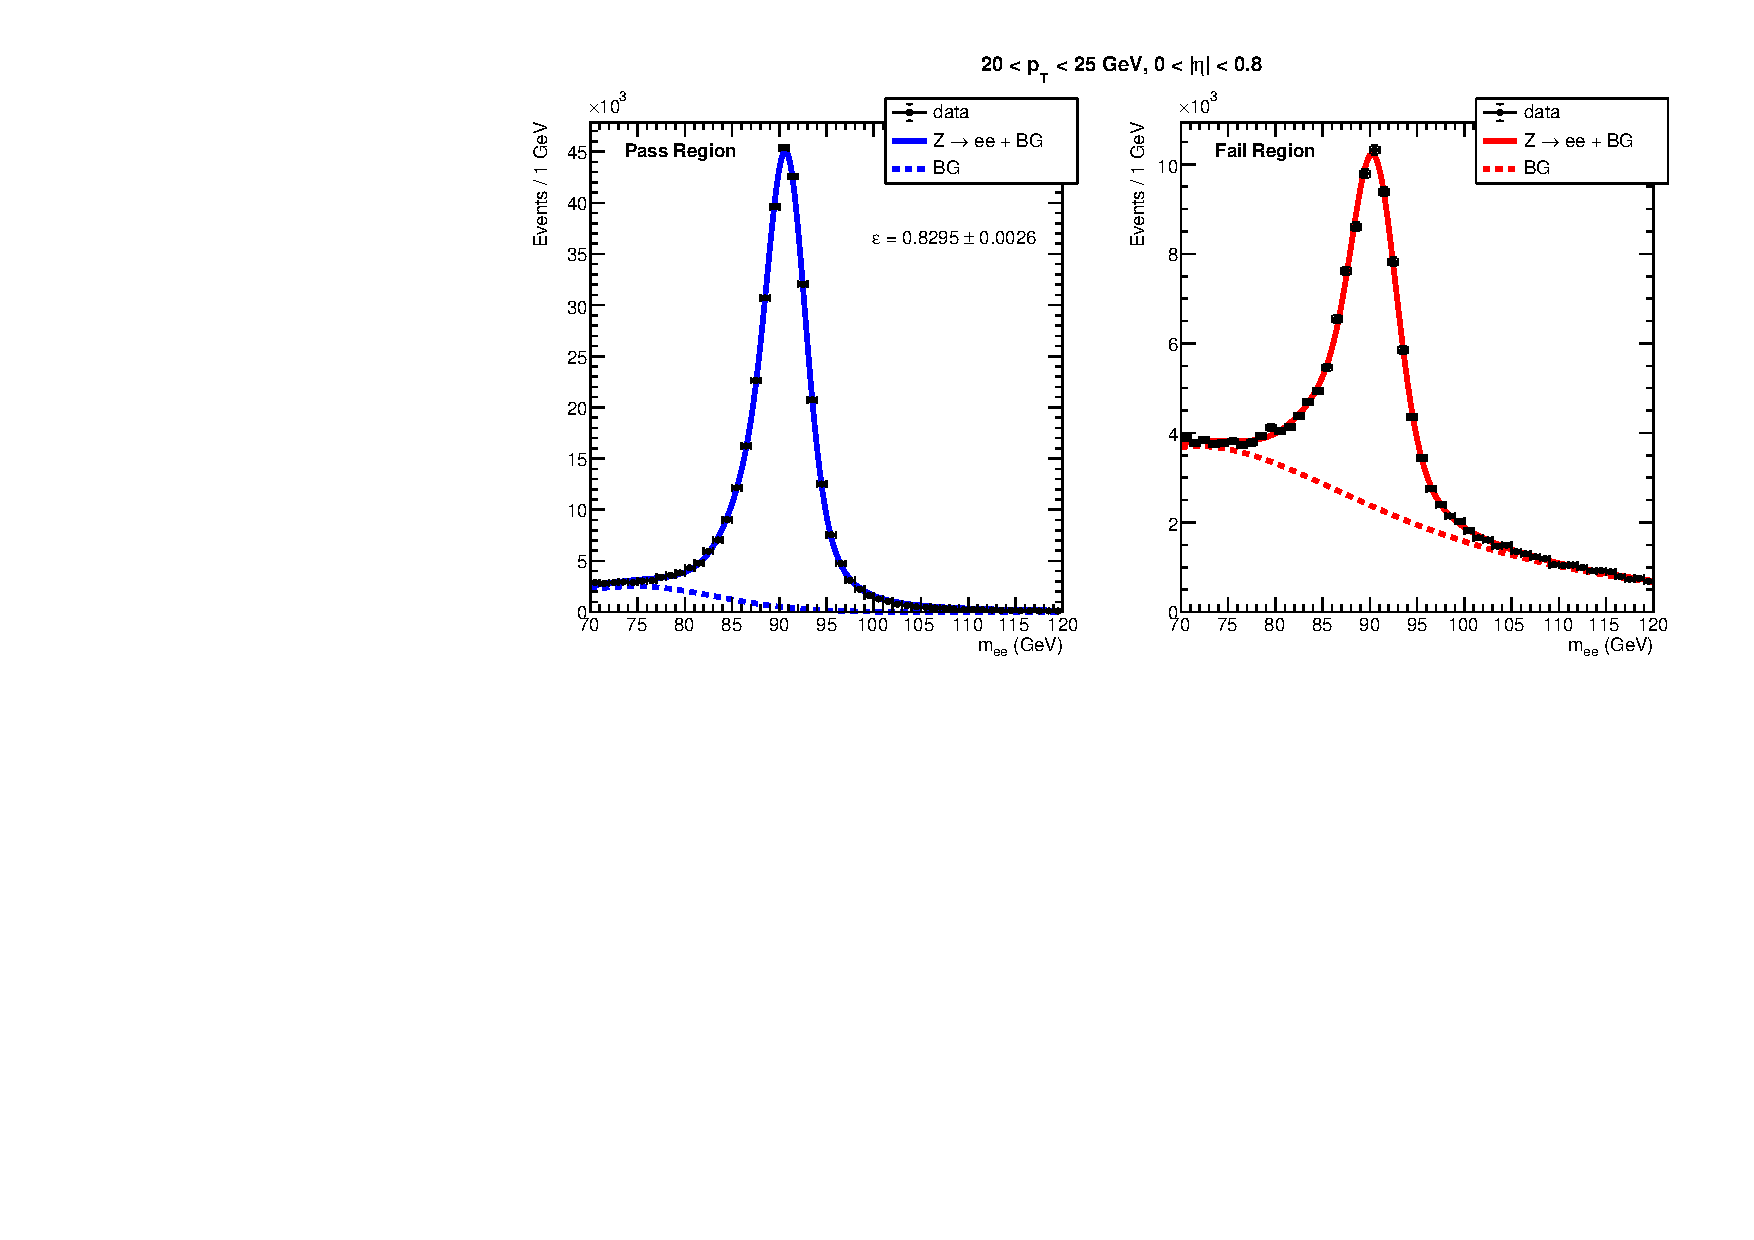
\includegraphics[width=\textwidth]{Figures/Chapter6/data_id_pt_20_to_25_eta_0.0_to_0.8_tpzee_tightTag.pdf}
    \caption[Impact of tag-and-probe configuration variations on efficiency extraction.]{Impact of tag-and-probe configuration variations on the measurement of electron identification efficiency in the $p_{\mathrm{T}}$ bin $20–25\GeV$ and $|\eta|$ region 0.0–0.8. Shown are invariant mass distributions and corresponding fits for a tighter tag lepton $p_\text{T}$ selection (+5\GeV). These are compared to the nominal configuration shown in Fig.~\ref{Figure:Chapter6-TagAndProbeFits_Nominal}.}
    \label{Figure:Chapter6-TagAndProbeFits_Alternative}
\end{figure}

\subsection{Hadronic taus}

\subsubsection{Identification and energy Scale}
\label{Section:Chapter6_Tau_ID_ES}

Reliable modelling of $\PGt_h$ candidates is essential for accurate signal and background estimation in this analysis. As with electrons and muons (see Sections~\ref{Section:Electron_Identification} and~\ref{Section:Muon_Identification}), data-to-simulation corrections are applied in the form of SFs. These corrections are derived centrally by the \ac{CMS} collaboration~\cite{DeepTau_24-001} and are therefore only summarised here.

Identification \acp{SF} are derived using a tag-and-probe method similar to that described for light leptons. In this case, $\PZ/\gamma^* \to \tau_\mu \tau_h$ events are used, where the muon serves as the tag and the $\PGt_h$ candidate as the probe. The visible mass of the muon–tau system, $m_{\text{vis}}$, is used as the primary observable. A binned maximum-likelihood fit to the $m_{\text{vis}}$ distribution, performed in the range $50 < m_{\text{vis}} < 150\GeV$, is used to extract the \ac{SF} by comparing yields in data and simulation. To improve the robustness of the derivation, the fit is performed simultaneously with a control region enriched in $\PZ/\gamma^* \to \mu\mu$ events. The \ac{DY} yield is treated with a common rate parameter across both regions, while the $\PGt_h$ ID \ac{SF} is treated as the parameter of interest. Systematic uncertainties, including muon efficiency, luminosity, background normalisation, and \ac{MC} statistics, are included as nuisance parameters. The resulting SFs are binned in \ac{HPS}-assigned \acp{DM} for $\pt^{\tauh} > 20\GeV$, accounting for variations across decay topologies and kinematic regions. 

In parallel, the \ac{TES} is extracted using external template fits. For each $\PGt_h$ \ac{DM}, a set of $m_{\text{vis}}$ templates is generated with varied \ac{TES} values, and the best-fit value is determined via a likelihood scan. This \ac{TES} correction is then applied by shifting the four-momentum of $\PGt_h$ matched to genuine $\PGt_h$ decays at generator level. The extracted values are typically within $\pm 2\%$, reflecting the excellent agreement between data and simulation in \ac{CMS} $\PGt_h$ energy reconstruction. The \ac{TES} correction is fixed when extracting the ID SFs.

\subsubsection{Trigger}

Trigger efficiency corrections for $\PGt_h$ candidates are also derived using $\PZ/\gamma^* \to \tau_\mu \tau_h$ events, exploiting the clean topology and well-identified muon leg. As with the identification and energy scale corrections, these are provided centrally by the \ac{CMS} collaboration and are therefore only summarised here.

The efficiencies are measured using a tag-and-probe technique similar to that described for electrons and muons in Section~\ref{Section:Chapter6_LightLepton_Corrections}. The muon serves as the tag, while the hadronic tau is treated as the probe. To avoid introducing biases on the probe leg, dedicated \textit{monitoring triggers} are employed. These triggers impose stringent requirements on the muon while emulating the trigger logic applied to the tau leg, enabling an unbiased measurement of tau trigger performance.

Separate corrections are derived for lepton+tau and double-tau triggers. The resulting \acp{SF} are applied to simulated events to correct for residual mismodelling in the trigger response.

\subsubsection{Lepton misidentification rates and energy scale}
\label{Section:Chapter6_Lepton_MisID_SF}

As introduced in Section~\ref{Section:Chapter6_Backgrounds}, prompt electrons and muons may be misidentified as $\PGt_h$ candidates by the DeepTau algorithm. Corrections for these misidentification rates are provided centrally by the \ac{CMS} collaboration and are summarised here.

A tag-and-probe technique, similar in principle to that used for genuine leptons in Section~\ref{Section:Chapter6_LightLepton_Corrections}, is employed in $\PZ/\gamma^* \to ee$ and $\PZ/\gamma^* \to \mu\mu$ events. One lepton serves as the tag, while the other is required to be reconstructed as a $\tauh$ candidate. Events are then classified based on whether the probe passes the relevant DeepTau discriminator ($D_e$ or $D_\mu$). Misidentification rates are measured as a function of $\eta_{\tauh}$, and the data-to-simulation ratio defines the corresponding SFs. These are applied to simulated $\tauh$ candidates originating from misidentified electrons or muons, as identified through generator-level matching ($e \to \tauh$ or $\mu \to \tauh$). The extracted misidentification rate scale factors are generally close to unity, with deviations of order 10–20\% in certain $\eta$ regions or \acp{DM}, and are complemented by energy scale corrections within $\sim$5–10%.

\subsection{B-tagging efficiency}

To correct for differences in $b$-tagging performance between data and simulation, jet-level SFs derived centrally by the \ac{CMS} collaboration are applied. These SFs adjust the tagging efficiency for jets originating from $b$-quarks, $c$-quarks, and light-flavour partons. Rather than applying a global event weight, the tagging status of each jet is modified individually using a randomised procedure: jets are probabilistically promoted or demoted depending on whether the corresponding \ac{SF} is greater or less than one. This approach ensures that the corrected jet collection reproduces data-like behaviour and can be used directly in event selection and categorisation without introducing additional per-event weights.

% This method is beneficial for analyses where the b-tag multiplicity defines the event category, since it allows for natural migration between categories and avoids complications associated with weighted event yields. However, it is not recommended in analyses that rely on variables which could become ill-defined when upgrading untagged jets—such as those involving secondary vertex information—since upgraded jets lack associated vertex reconstruction. Care must also be taken when SFs cross unity due to systematic variations, as this may affect the stability of such variables.


\section{Background modelling}
\label{Section:Chapter6_Background_Modelling}

As described in Section~\ref{Section:Chapter6_Backgrounds}, several processes can mimic the $Z^* \to \phi A \to 4\PGt$ signal signature, either through the presence of genuine $\PGt$ leptons, misidentified jets or light leptons reconstructed as $\PGt_h$ candidates, or a combination of both. This section outlines the strategies used to model these backgrounds and validate their contributions. For clarity, background processes are grouped into three main categories:


\begin{enumerate}[label=(\roman*)]

\item \textbf{Genuine-$\PGt$ backgrounds:} Events containing only genuine $\PGt$ leptons, primarily from $\PZ\PZ \to 4\PGt$, form an irreducible background and are estimated using simulation.

\item \textbf{Jet $\to \PGt_h$ misidentification:} Backgrounds with one or more jets misidentified as $\PGt_h$ candidates are modelled using a data-driven fake factor method.

\item \textbf{Lepton $\to \PGt_h$ misidentification:} Although subdominant, backgrounds from electrons or muons misidentified as $\PGt_h$ candidates can affect specific channels. These are estimated using simulation with dedicated corrections, as detailed in Section~\ref{Section:Chapter6_Lepton_MisID_SF}.

\end{enumerate}

\subsection{\texorpdfstring{Genuine-\boldmath{$\PGt$} backgrounds from $\PZ\PZ$}{Genuine tau backgrounds from ZZ}}
\label{Section:Chapter6_GenuineBackground}


These backgrounds arise predominantly from quark–antiquark annihilation, with a smaller contribution from gluon–gluon fusion. As discussed in Section~\ref{Section:Chapter6_Backgrounds}, these backgrounds, owing to their fully leptonic final state and close kinematic resemblance to the signal, are particularly challenging to suppress. As listed in Table~\ref{Table:Chapter6_SimulatedBackgrounds}, the quark-initiated process is simulated using \POWHEG at \ac{NLO} in \ac{QCD}, while the gluon-initiated component is generated at \ac{LO} with \PYTHIA. To account for missing higher-order effects, both samples are corrected using multiplicative $\mathcal{K}$-factors~\cite{Kfactors_ZZ} applied as a function of the four-lepton invariant mass, $m_{4\ell}$:

\begin{itemize}
\item Quark-initiated $\PZ\PZ$:  A mass-dependent \ac{NLO}-to-\ac{NNLO} \ac{QCD} $\mathcal{K}$-factor derived from \POWHEG~2.0\cite{Powheg_1,Powheg_2} is applied, with a typical value of around 1.2 across the relevant phase space.
\item Gluon-initiated $\PZ\PZ$: A larger $\mathcal{K}$-factor, typically 2.0, is applied to match \ac{NNLO} predictions from \textsc{HNNLO v2}\cite{PhysRevLett.98.222002}.
\end{itemize}

Simulation is validated in a control region enriched in $\PZ\PZ \to \mu^+\mu^-\mu^+\mu^-$, which provides a clean signature with minimal background contamination. The standard object selection criteria (see Table~\ref{Table:Chapter6_ObjectSelectionSummary}) are applied, with one targeted modification: the muon isolation requirement is relaxed to $I^\mu_\text{PF} < 0.35$ to enhance statistical precision. The total charge of the four-muon system is also required to be zero. Additionally, the trigger configuration used in this region is detailed in Table~\ref{Table:Chapter6_TriggersPerChannel}. Figure~\ref{Figure:Chapter6_ZZ_KfactorImpact} illustrates how applying $\mathcal{K}$-factors improves the agreement between simulation and data in the invariant mass distribution of the four-muon system.

\begin{figure}[!htbp]
        \centering
        % First row
        \begin{subfigure}[b]{0.49\textwidth}
            \centering
            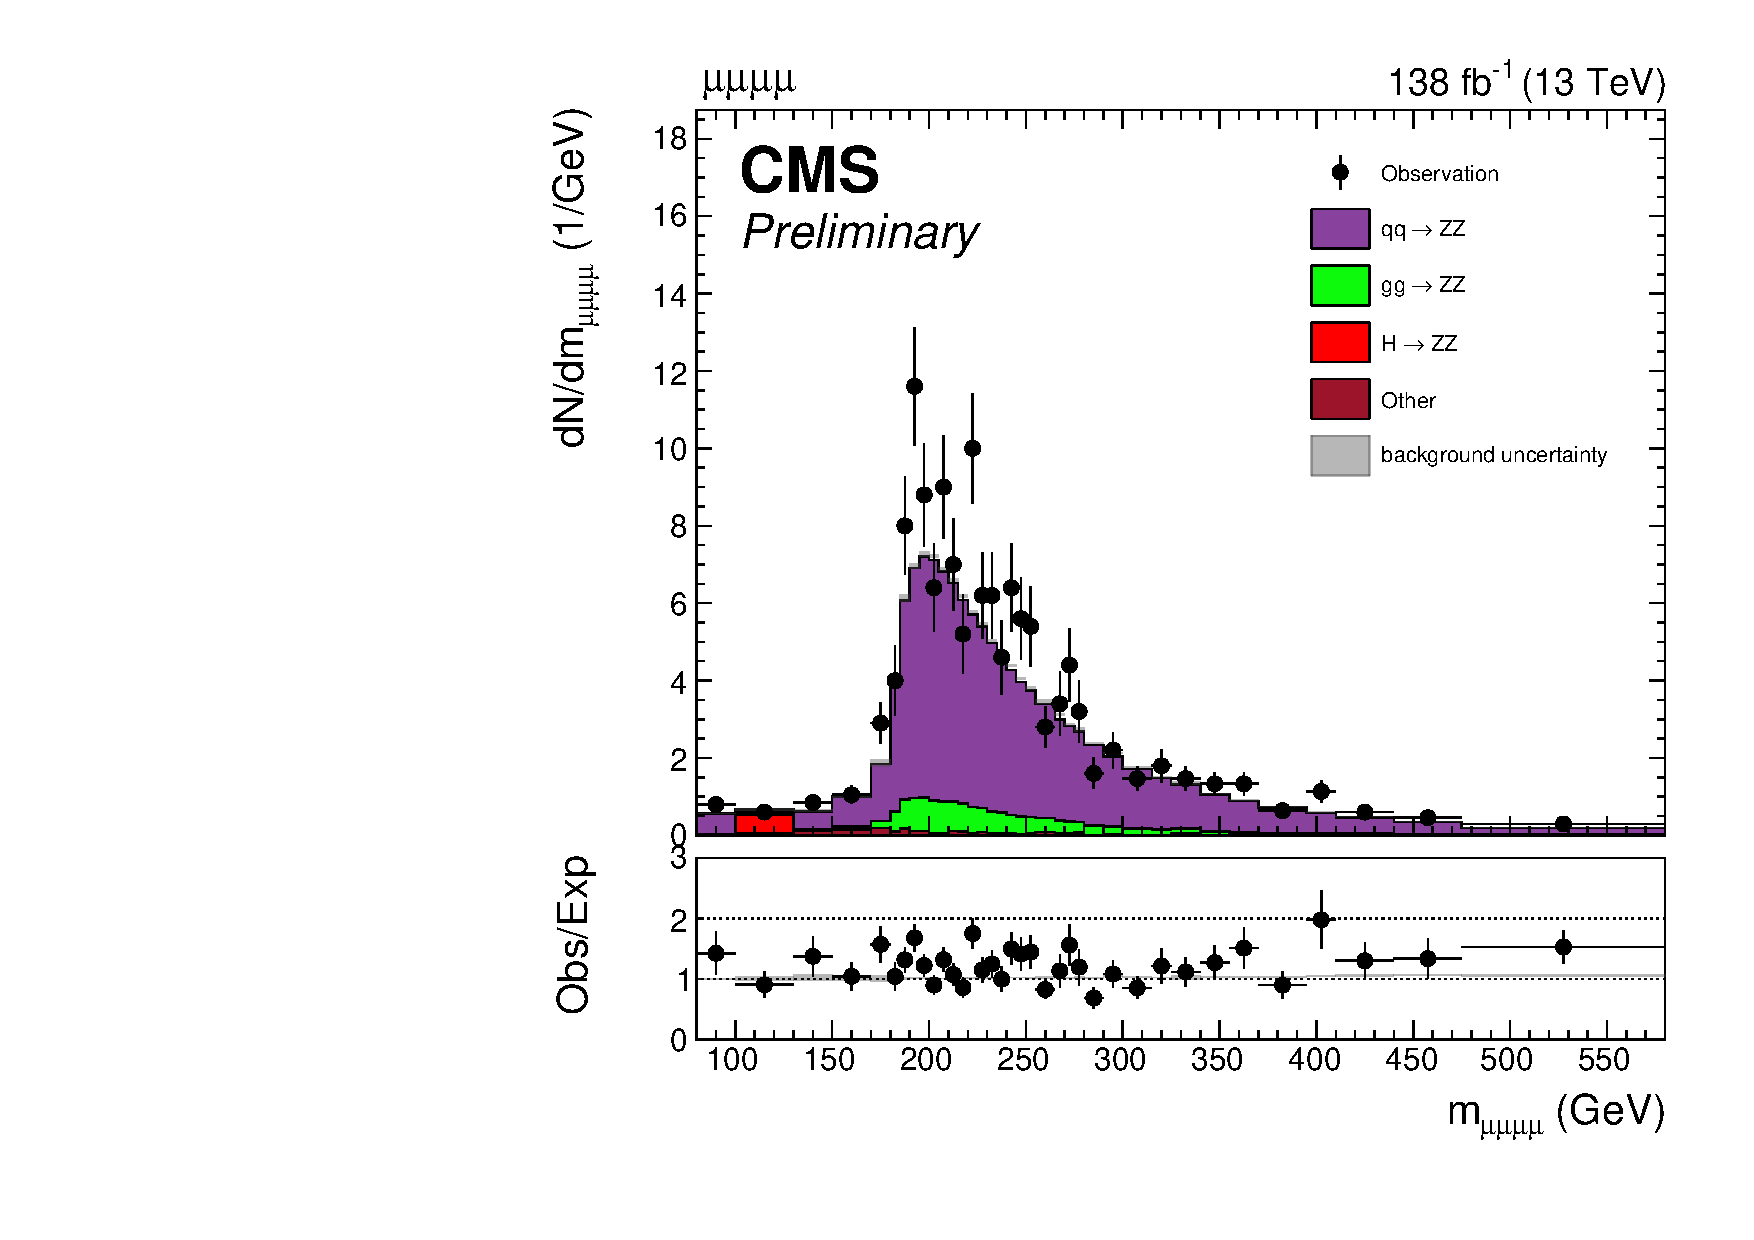
\includegraphics[width=\textwidth]{Figures/Chapter6/mmmm_wo_kfactors.pdf}
            \caption{}
        \end{subfigure}
        \vspace{0.5cm}
        \begin{subfigure}[b]{0.49\textwidth}
            \centering
            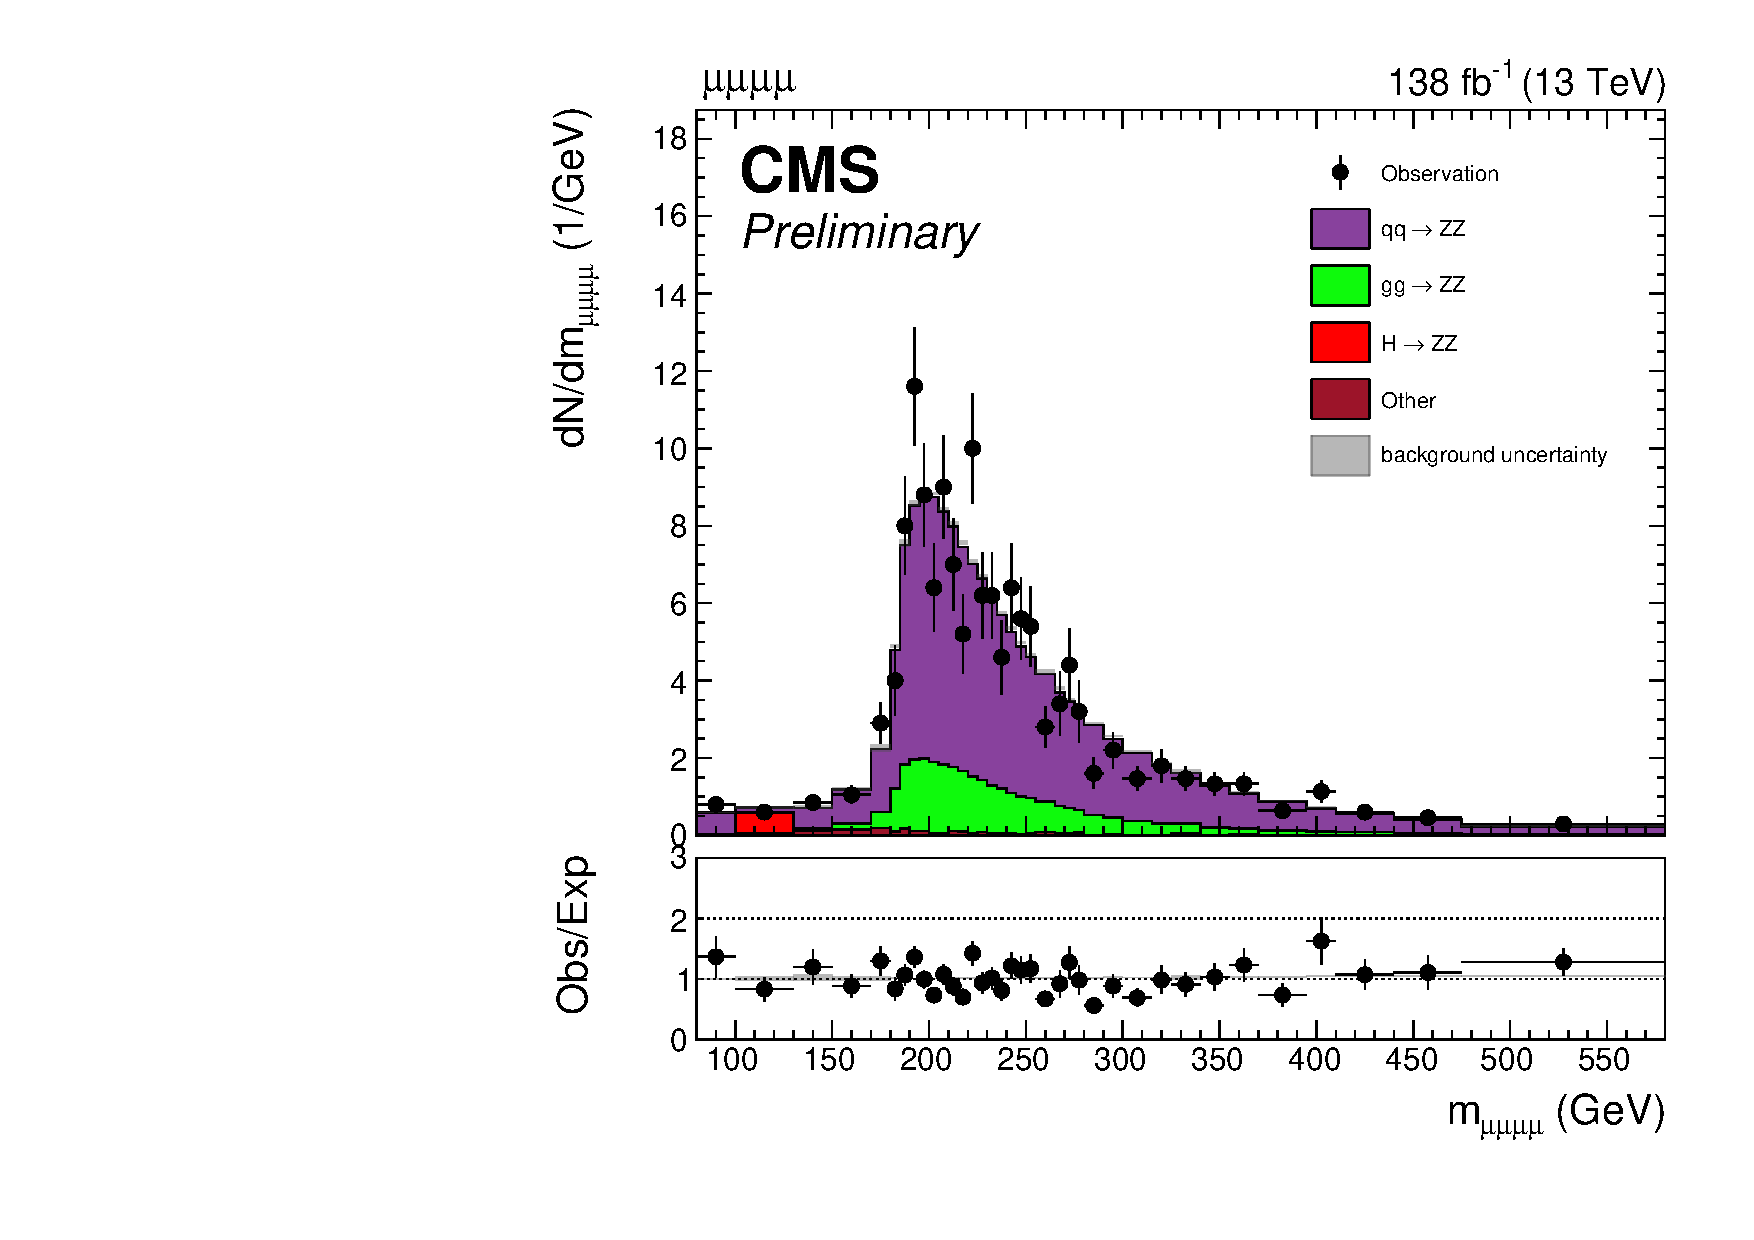
\includegraphics[width=\textwidth]{Figures/Chapter6/mmmm_with_kfactors.pdf}
            \caption{}
        \end{subfigure}
    \caption[Impact of $\mathcal{K}$-factors on the $\PZ\PZ$ background prediction in the four-muon control region.]{Impact of $\mathcal{K}$-factors on the $\PZ\PZ$ background prediction in the four-muon control region. Shown are the invariant mass distributions of the $\mu^+\mu^-\mu^+\mu^-$ system before (\textbf{a}) and after (\textbf{b}) applying $\mathcal{K}$-factors.}
    \label{Figure:Chapter6_ZZ_KfactorImpact}
\end{figure}

While $\PZ\PZ$ constitutes an irreducible background, it can still be reduced through targeted kinematic selections. For example, in the $\PGt_e\PGt_h\PGt_h\PGt_h$ channel, signal events tend to exhibit harder $p_{\mathrm{T}}$ spectra for subleading leptons. The object selection thresholds conveniently exploit this difference. As illustrated in Fig.~\ref{Figure:Chapter6_ThirdLepPt}, applying a $p_{\mathrm{T}}$ cut at $20\GeV$ significantly reduces this background while preserving the majority of the signal.

\begin{figure}[!htbp]
    \centering
    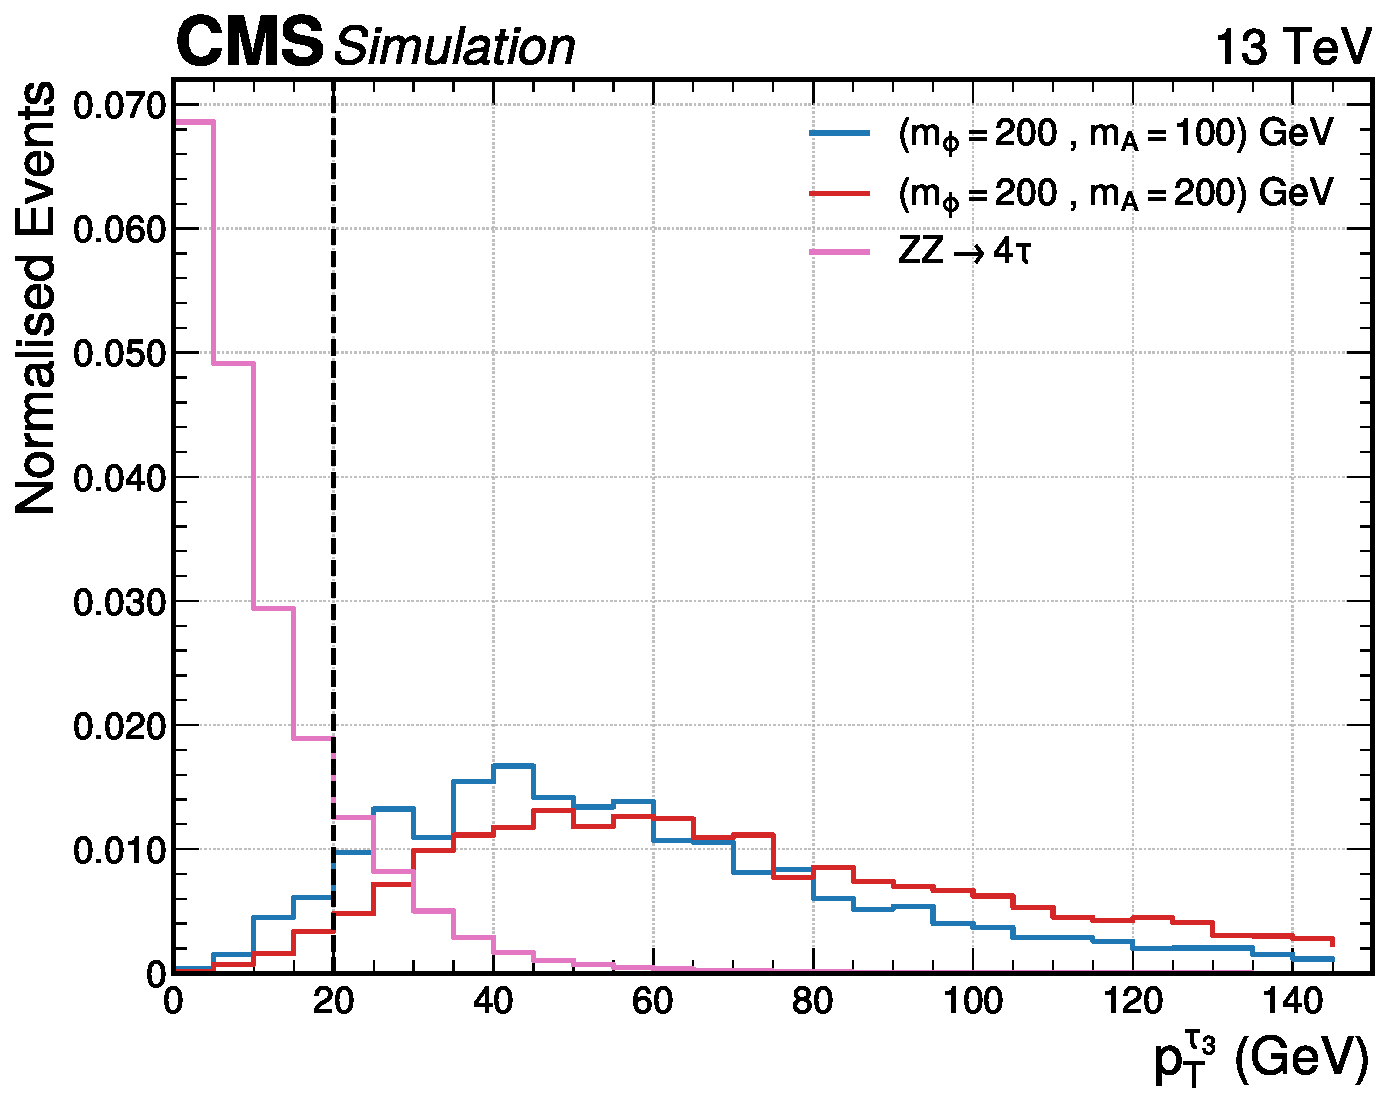
\includegraphics[width=0.6\textwidth]{Figures/Chapter6/ZZ_OfflineCutImpact.pdf}
    \caption[$p_{\mathrm{T}}$ spectrum of the third lepton in the $\PGt_e\PGt_h\PGt_h\PGt_h$ channel.]{Distribution of the transverse momentum of the third lepton in the $\PGt_e\PGt_h\PGt_h\PGt_h$ channel, comparing the expected $\PZ\PZ$ background to the signal prediction. The solid line at $20\GeV$ region indicates the $p_{\mathrm{T}}$ selection threshold applied.}
    \label{Figure:Chapter6_ThirdLepPt}
\end{figure}

\subsection{\texorpdfstring{Background from Jets Misidentified as $\PGt_h$ (Jet $\to \PGt_h$)}{Background from Jets Misidentified as hadronic taus}}

\label{Section:Chapter6_JetToTauBackground}

This section discusses how the background from jets misidentified as $\PGt_h$ candidates is modelled. These backgrounds arise from misidentified jets from processes such as the ones outlined in Section~\ref{Section:Chapter6_Backgrounds}. Such misidentifications are particularly problematic to model in simulation, as the jet-to-$\PGt_h$ misidentification rate is poorly described in \ac{MC} simulations. Moreover, the small probability of such a jet misidentification makes it necessary to generate high-statistics \ac{MC} samples, which come with a significant computational expense. These limitations and the difficulty in capturing the full range of misidentification scenarios in simulation motivate the use of a data-driven approach, such as the Fake Factor ($F_F$) method.

\subsubsection{Classical Fake Factor Method}
\label{Section:Chapter6_FakeFactors_Classical}

The classical $F_F$ approach begins by defining a dedicated \ac{DR}, enriched in jet$\to\PGt_h$ events. Any non-jet$\to\PGt_h$ contributions are estimated using simulation and subtracted to isolate the misidentified component, ensuring a pure region. In this region, the $F_F$ is computed as the ratio of events passing a \texttt{Nominal} tau ID requirement to those failing it but satisfying a looser \texttt{Alternative} ID:

\begin{equation}
F_F = \frac{\mathcal{N}(\texttt{Nominal})}{\mathcal{N}(\texttt{Alternative and not Nominal})}
\end{equation}

The choice of the alternative identification requirement introduces a trade-off. Looser identification thresholds reduce the statistical uncertainty by increasing the number of events in the denominator. However, this comes at the cost of increased systematic uncertainty, as the looser $\PGt_h$ candidates are less representative of those in the \ac{SR}. 

Regarding its determination, the $F_F$ is computed differentially in key variables such as $p_\text{T}$, jet multiplicity ($\mathcal{N}_{\text{jets}}$), and other observables that parametrise the misidentification rate. Since the $F_F$ can also depend on the definition of the \ac{DR}, additional corrections are often derived in sideband regions to mitigate residual dependencies and improve the robustness of the estimate. The $F_F$ is then applied to the \ac{AR}, which is constructed to resemble the \ac{SR}. Specifically, the \ac{AR} requires the $\PGt_h$ candidates to pass the \texttt{Alternative} ID and fail the \texttt{Nominal} one. This enables a fully data-driven estimate of the jet-induced background in the \ac{SR}.

Despite its simplicity and robustness, the classical method faces several limitations:

\begin{itemize}
\item \textit{Curse of dimensionality}: Including more variables in the parameterisation rapidly inflates the number of bins, leading to sparse statistics and unstable estimates.

\item \textit{Correlations}: Variables not explicitly included in the fit may be poorly modelled. Corrections in one observable can worsen agreement in another, highlighting the limitations of low-dimensional approaches that fail to capture correlations.

\item \textit{Scalability in multi-$\PGt_h$ final states}: In channels like $\PGt_h \PGt_h \PGt_h \PGt_h$, the method becomes increasingly cumbersome. A separate $F_F$ must be computed for each $\PGt_h$ candidate, applied iteratively. This procedure becomes statistically challenging in low-yield regimes and complicates the estimate.
\end{itemize}

These challenges were noted in previous \ac{CMS} analyses of ditau final states~\cite{CMS:2022goy,Mb:2022rxu}, where a $F_F$ was typically derived for, and applied to, the leading $\PGt_h$ candidate. This approach could not account for cases in which the leading object was genuine and the subleading object was a misidentified jet. Such events had to be modelled using simulation. While this simplification was acceptable in those studies due to the subdominant contribution of such configurations, it becomes insufficient in this analysis, where final states often involve multiple misidentified $\PGt_h$ candidates. A more general, high-dimensional approach is therefore required to reliably account for all sources of jet$\to\PGt_h$ misidentification.


\subsubsection{Machine Learning-based reweighting}
\label{Section:Chapter6_FakeFactors_BDT}

To overcome the limitations of binning-based methods, misidentification rates can be estimated using \ac{SR}-based density ratio estimation. The objective is to model the misidentification rate as a function of multiple observables. Mathematically, this corresponds to estimating the ratio of probability densities $f_{\text{pass}}(x)/f_{\text{fail}}(x)$.

\begin{equation_pad}
\frac{f_{\text{pass}}(x)}{f_{\text{fail}}(x)} \sim \frac{p_{\text{pass}}(x)}{p_{\text{fail}}(x)}.
\end{equation_pad}

This ratio can be approximated using classifiers such as \acp{BDT}, where the class probabilities serve as a proxy for the density ratio. However, standard classifiers often underperform in regions where the density ratio is large (\ie where one class dominates). In such regions, the classification task becomes trivial, and the model focuses its learning on harder, more ambiguous regions where classes are balanced. These easy-to-classify regions receive little weight in the loss function (typically cross-entropy), leading to poor modelling precisely where accurate reweighting is most critical.

To mitigate this, a custom objective function is introduced that directly targets discrepancies between the pass and fail distributions. In tree-based models, this objective is optimised over sets of events grouped into leaves\footnote{Leaves are the terminal nodes of a decision tree; each leaf contains events satisfying the same set of decision rules.}. This objective function is the symmetrised $\chi^2$ metric, which prioritises leaves with the largest differences between the two samples:

\begin{equation_pad}
    \chi^2 = \sum_{\text{leaf}} \frac{(w_{\text{leaf}, \text{fail}} - w_{\text{leaf}, \text{pass}})^2}{w_{\text{leaf}, \text{fail}} + w_{\text{leaf}, \text{pass}}}
\end{equation_pad}

where $w_{\text{leaf}, \text{fail}}$ and $w_{\text{leaf}, \text{pass}}$ are the total event weights in each leaf from the fail and pass samples, respectively. Maximising this objective during training steers the model toward the regions most relevant for improving reweighting accuracy.

Training proceeds in a boosting-like fashion, where a series of shallow decision trees is built sequentially. Each tree addresses discrepancies not corrected by previous ones. At each iteration, the following steps are performed:

\begin{enumerate}[label=(\roman*)]
    \item A shallow decision tree that maximises the symmetrised $\chi^2$ is built.
    \item For each leaf, the log-ratio of total weights ($r_\text{leaf}$) is computed:
    \item The weights of fail-sample events in each leaf are updated: $w = w \times e^{r{_\text{leaf}}}$.
\end{enumerate}

This procedure is iterated multiple times, allowing the model to refine the reweighting progressively by targeting residual discrepancies in each step.

\subsubsection{Fitting and Parametrisation}
\label{Section6:Fitting_Parametrisation}
Having introduced the \ac{ML}-based reweighting approach, this section outlines its implementation in the context of this analysis. This includes the definition of fitting regions and the choice of input variables for training. As described in Section~\ref{Section:Chapter6_FakeFactors_Classical}, the classical $F_F$ method relies on defining a set of control regions. These regions can be organised into an ABCD-style framework, as illustrated in Fig.~\ref{Figure:Chapter6_ABCD}, with sidebands constructed from variables such as hadronic tau identification and total charge.

\begin{figure}[!htbp]
\centering
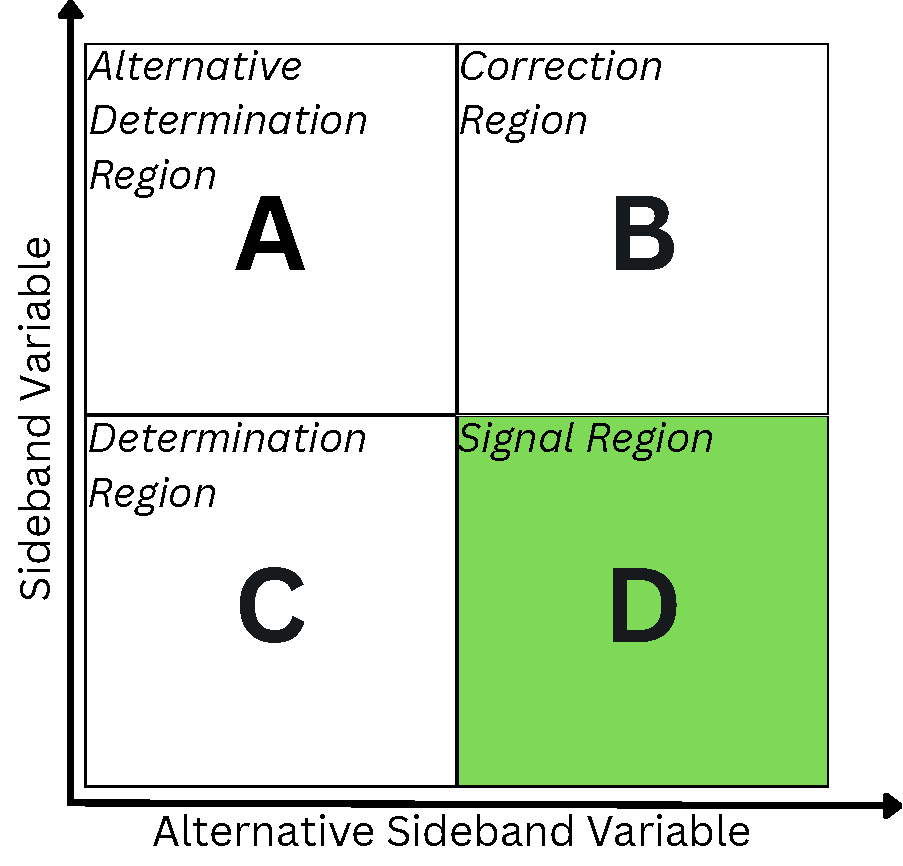
\includegraphics[width=0.6\textwidth]{Figures/Chapter6/ABCD.pdf}
\caption[ABCD-style region definition for fake factor estimation.]{Schematic illustration of an ABCD-style region definition used in the fake factor method.}
\label{Figure:Chapter6_ABCD}
\end{figure}

The channel-specific sideband selections used to define these regions are summarised below:

\begin{enumerate}[label=(\roman*)]
    \item For the channels: $\PGt_e\PGt_h\PGt_h\PGt_h$, $\PGt_e\PGt_e\PGt_h\PGt_h$, $\PGt_e\PGt_\mu\PGt_h\PGt_h$, $\PGt_\mu\PGt_h\PGt_h\PGt_h$, $\PGt_\mu\PGt_\mu\PGt_h\PGt_h$, and $\PGt_h\PGt_h\PGt_h\PGt_h$:
    \begin{itemize}
    \item \textbf{Region A (\ac{SR}-like)}: \\
    All alternative\footnote{``Alternative'' refers to all other hadronic taus in the event for which the $F_F$ is not currently being derived.} hadronic taus pass the \texttt{Nominal} tau ID; $\sum q_{\PGt_h} = 0$.

    \item \textbf{Region B (Inverted Identification)}: \\
    At least one alternative hadronic tau fails the \texttt{Nominal} tau identification but passes the \texttt{Alternative} selection; $\sum q = 0$.

    \item \textbf{Region C (Inverted Charge)}: \\
    All alternative $\PGt_h$ hadronic taus pass the \texttt{Nominal} tau ID; charge sum requirement is $\sum q \neq 0$.

    \item \textbf{Region D (Inverted ID and Charge)}: \\
    At least one alternative hadronic tau fails the \texttt{Nominal} tau ID but passes the \texttt{Alternative} selection; $\sum q \neq 0$.
    \end{itemize}

    \item For the $\PGt_h\PGt_h\PGt_h$ channel, the same ID criteria apply, but the charge requirement is modified:
    \begin{itemize}
        \item \textbf{Region A/B}: $|\sum q \,| = 1$
        \item \textbf{Region C/D}: $|\sum q\,| \neq 1$
    \end{itemize}
\end{enumerate}

While this framework is conceptually straightforward for deriving the $F_F$ for a single $\PGt_h$ candidate, it becomes increasingly complex in multi-$\PGt_h$ events as discussed in Section~\ref{Section:Chapter6_FakeFactors_Classical}. Each candidate must be treated separately, with its own ABCD categorisation defined in terms of the others. This results in multiple overlapping sets of control regions that must be constructed within the same event.

The \ac{ML} approach circumvents these issues entirely by eliminating the need for explicit ABCD definitions. Each $\PGt_h$ candidate is treated as an independent training instance, contributing a single row to the training dataset. Both candidate-level and event-level features, including those used in traditional ABCD axes, are passed directly to the model. This enables the algorithm to learn a flexible, high-dimensional reweighting function across the entire parameter space without fragmenting the data. The features used for training are grouped as follows:

\begin{enumerate}[label=(\roman*)]

    \item \textbf{Properties of the target $\PGt_h$ candidate:} The target $\PGt_h$ candidate is characterised by several features: its \ac{HPS} \ac{DM}, $p_\text{T}^{\PGt_h}$,  $\eta$, electric charge, and whether it satisfies the relevant leg of the double-$\tau$ trigger. Additionally, the ratio of the $p_\text{T}$ of the seeding jet to that of the $\PGt_h$ candidate ($p_\text{T}^\text{jet} / p_\text{T}^{\PGt_h}$) is included.

    \item \textbf{Sideband-specific variables:}
    \begin{itemize}
        \item Total charge of all $\PGt_h$ candidates
        \item A boolean indicating whether the DeepTau discriminator of the alternative hadronic taus (sorted by $p_\text{T}$) passes the \texttt{Nominal} tau identification requirement
    \end{itemize}

    \item \textbf{Global event variables:}
    \begin{itemize}
        \item Data-taking period identifier
        \item $p_\text{T}$ rank of the target hadronic tau in the event
    \end{itemize}

\end{enumerate}

\subsubsection{\texorpdfstring{Non-jet$\to \PGt_h$ background removal}{Non-jet to hadronic tau background removal}}
\label{Section:Chapter6_BDT_NonJet_BkgRemoval}

As noted in Section~\ref{Section:Chapter6_FakeFactors_Classical}, backgrounds from non-jet$\to\PGt_h$ candidates are traditionally removed by subtracting simulated events from data at the histogram level. However, this approach is not compatible with the \ac{ML}-based method, which operates on full unbinned datasets and does not support negative event weights. One possible workaround is template matching, where a simulated non-jet$\to\PGt_h$ candidate for every matching data event is removed to emulate histogram subtraction at the event level. Yet, this method is computationally infeasible given the high dimensionality of the input space and the size of the datasets.

Instead, a binary \ac{BDT} is trained to distinguish jet$\to\PGt_h$ from non-jet$\to\PGt_h$ candidates, using the same input variables as the main reweighting model. This reduces the classification problem to a single discriminant: the \ac{BDT} score, which quantifies how ``non-jet$\to\PGt_h$-like'' each candidate is. The trained \ac{BDT} is applied to both simulation and data. A histogram of \ac{BDT} scores is constructed from simulated non-jet$\to\PGt_h$ candidates and normalised to the expected cross section, yielding a bin-by-bin prediction of the expected contamination in data. The same \ac{BDT} is then applied to data, and for each bin of the \ac{BDT} score distribution, data events falling within that range are randomly sampled and removed. This is repeated until the number of removed events matches the predicted contamination in that bin.

The result is a purified dataset of jet$\to\PGt_h$-like candidates, closely mimicking the effect of histogram-level subtraction but in a form that remains compatible with the \ac{ML}-based reweighting method. Figure~\ref{Figure:Chapter6_BDTPurificationExample} compares this strategy with the traditional subtraction method, demonstrating their agreement.

\begin{figure}[!htbp]
        \centering
        % First row
        \begin{subfigure}[b]{0.49\textwidth}
            \centering
            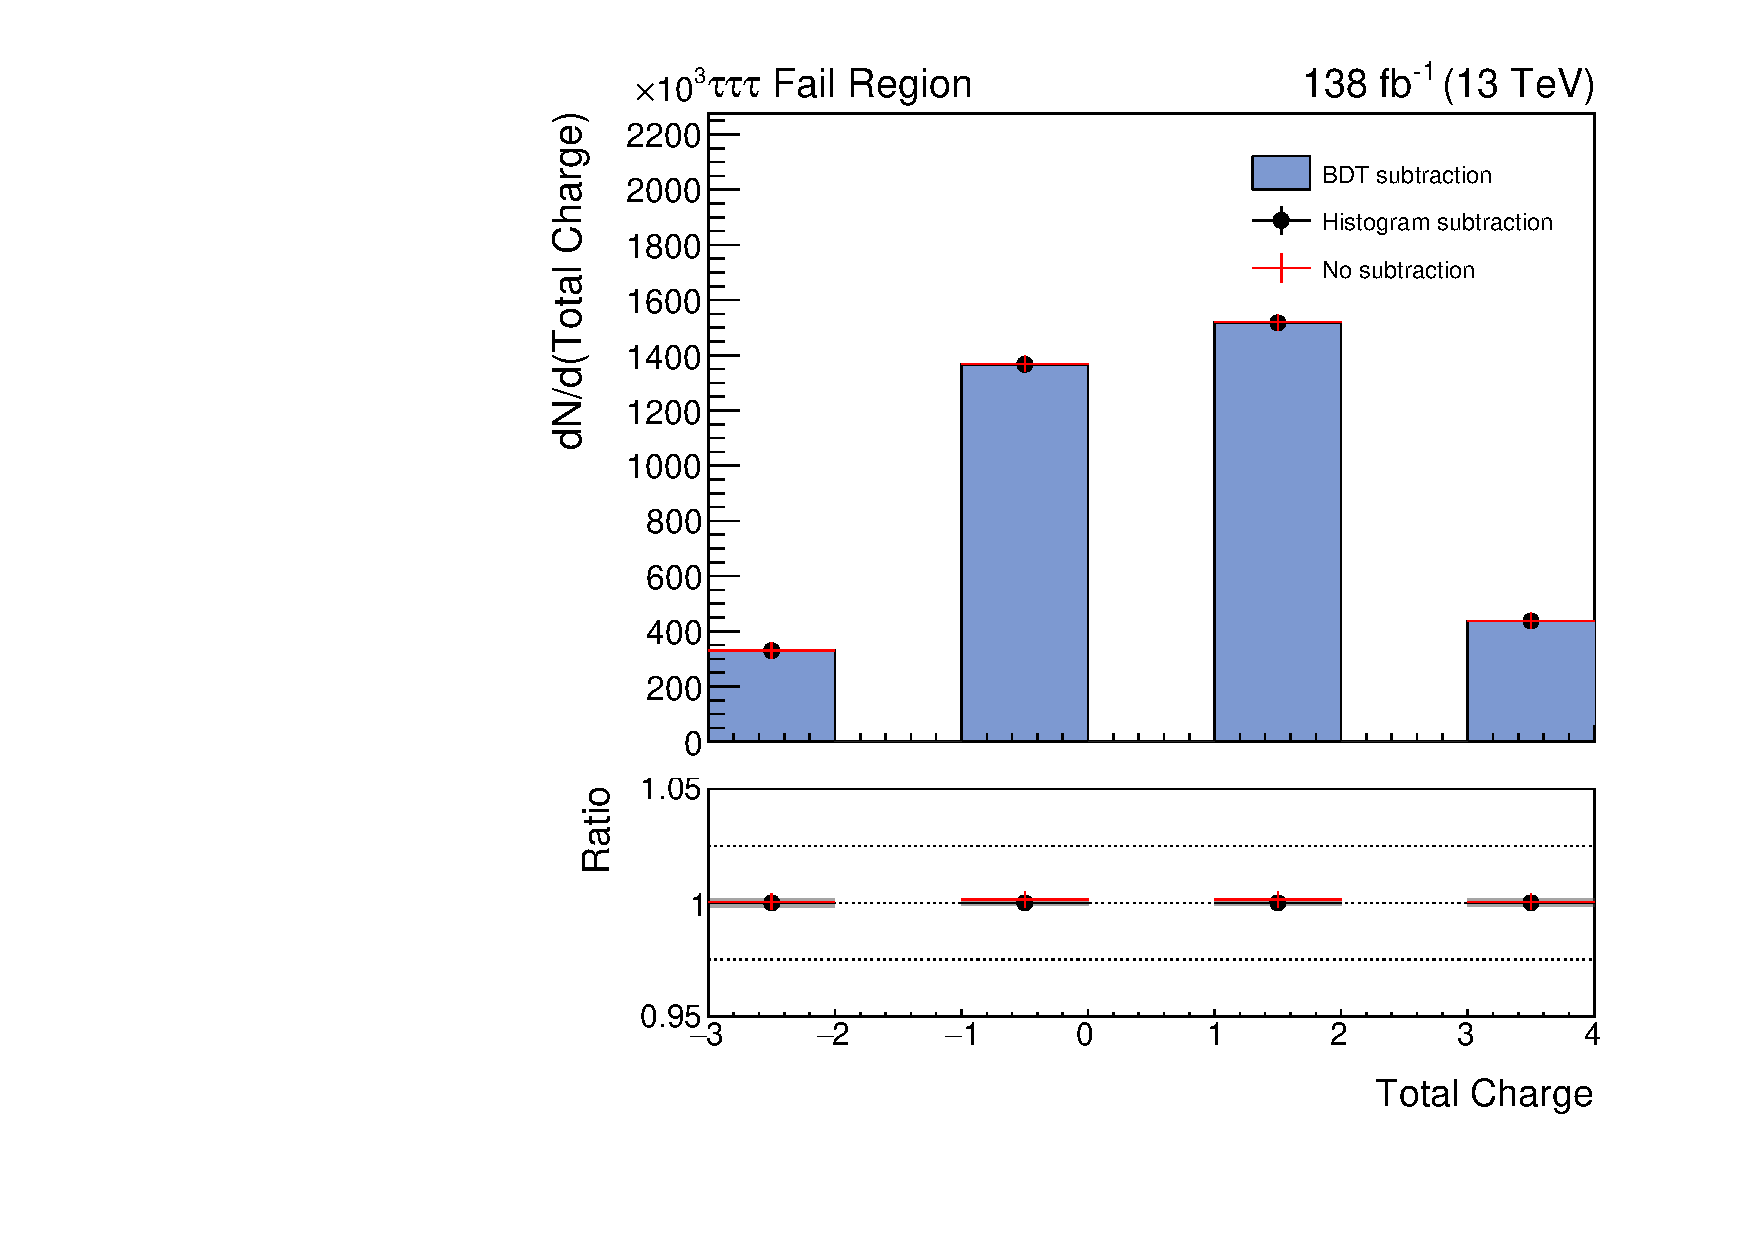
\includegraphics[width=\textwidth]{Figures/Chapter6/subtraction_plot_q_sum_ttt_fail.pdf}
            \caption{}
        \end{subfigure}
        \vspace{0.5cm}
        \begin{subfigure}[b]{0.49\textwidth}
            \centering
            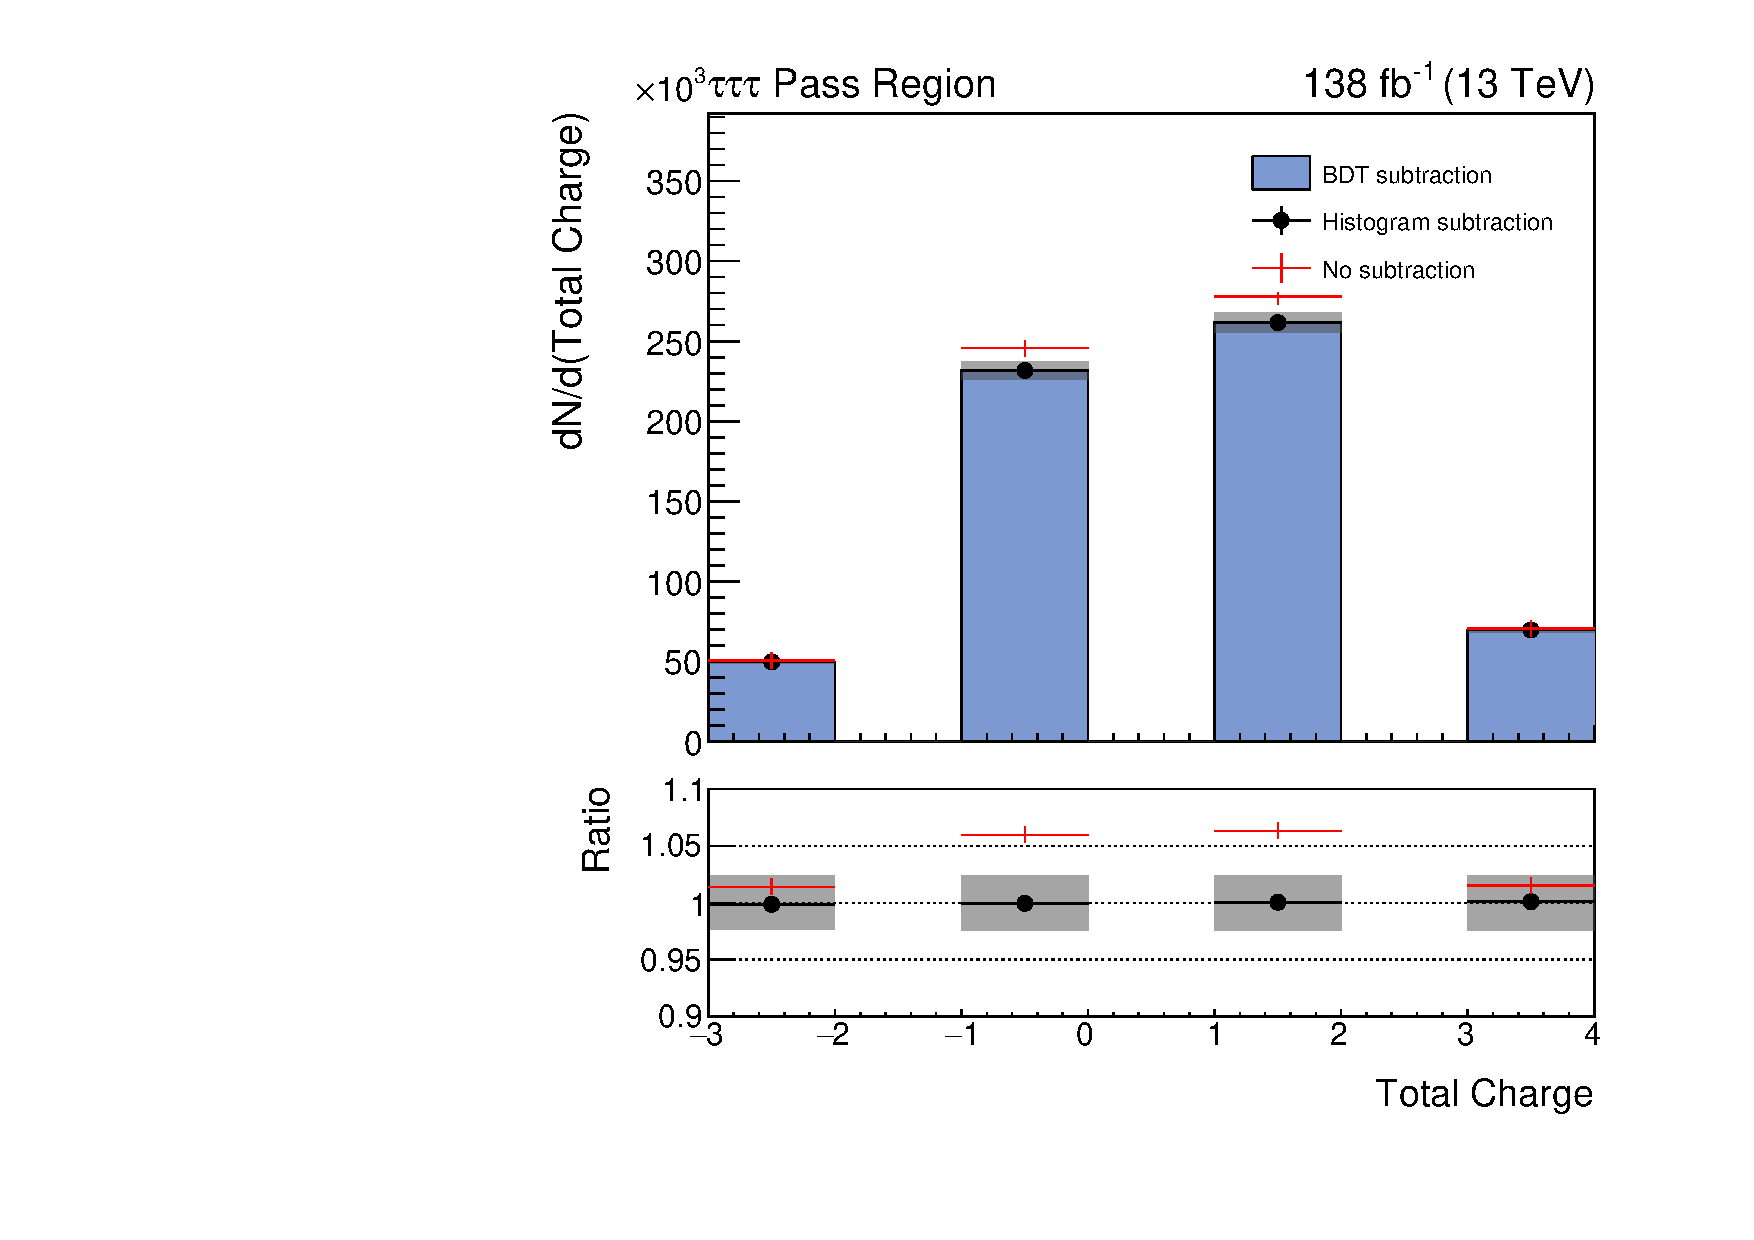
\includegraphics[width=\textwidth]{Figures/Chapter6/subtraction_plot_q_sum_ttt_pass.pdf}
            \caption{}
        \end{subfigure}
    \caption[Comparison of subtraction techniques applied to the total charge distribution of $\PGt_h$ candidates.]{Comparison of subtraction techniques applied to the total charge distribution of $\PGt_h$ candidates in the \textbf{(a)} fail and \textbf{(b)} pass regions.}

    \label{Figure:Chapter6_BDTPurificationExample}
\end{figure}

\subsubsection{\texorpdfstring{Application of the $F_F$}{Application of the Fake Factor}}
\label{Section:Chapter6_FF_Application}
As discussed in Section~\ref{Section6:Fitting_Parametrisation}, the \ac{ML}-based method enables the derivation of a $F_{F}^i$, for each $\PGt_h$ candidate $i$ in the event. However, in events containing multiple $\PGt_h$ candidates, care must be taken to account for all possible misidentification combinations without introducing overcounting. For example, applying $F_{F}^1$ only to the leading candidate neglects subleading misidentified contributions, while applying all $F_{F}^i$ simultaneously results in double-counting. To resolve this, additive and subtractive combinations of the $F_{F}^i$ are used to properly model the full jet$\to\PGt_h$ background. The application logic for events with two and three $\PGt_h$ candidates is summarised in Tables~\ref{Table:Chapter_6_FFApplication_2Taus} and~\ref{Table:Chapter_6_FFApplication_3Taus}, respectively.

\begin{table}[!htbp]
\centering
\renewcommand{\arraystretch}{1.5} % Increase row height
\setlength{\tabcolsep}{12pt} % Increase column width
\arrayrulecolor{black} % Ensure outer border is black
\begin{tabular}{cccc}
\hline
Region & $\PGt_h^1$ \textcolor{red}{$\PGt_h^2$} & \textcolor{red}{$\PGt_h^1$} $\PGt_h^2$ & \textcolor{red}{$\PGt_h^1 \PGt_h^2$} \\ \hline

$F_F^1$ & 0 & 1 & 1 \\
\arrayrulecolor{lightgray} \hline

$F_F^2$ & 1 & 0 & 1 \\
\arrayrulecolor{lightgray} \hline

$-F_F^1 \times F_F^2$ & 0 & 0 & 1 \\
\arrayrulecolor{black} \hline
Combined & 1 & 1 & 1 \\
\end{tabular}
\caption[Combinatorial application of Fake Factors for two $\PGt_h$ candidates.]{
Combinatorial application of $F_F^i$ in events with two $\PGt_h$ candidates. Each column represents a control region where different combinations of candidates are treated as misidentified jets (shown in red). For example, $\PGt_h$\textcolor{red}{$\PGt_h$} indicates a region where the second candidate is assumed to be misidentified.}
\label{Table:Chapter_6_FFApplication_2Taus}
\end{table}


\begin{table}[!htbp]
\centering
\renewcommand{\arraystretch}{1.5} % Increase row height
\setlength{\tabcolsep}{10pt} % Increase column width
\arrayrulecolor{black} % Ensure outer border is black
\begin{tabular}{ccccccc}
\hline
Region & \textcolor{red}{$\PGt_h^1$} $\PGt_h^2$ $\PGt_h^3$ & \textcolor{red}{$\PGt_h^1 \PGt_h^2$} $\PGt_h^3$ & \textcolor{red}{$\PGt_h^1 \PGt_h^2 \PGt_h^3$} & $\PGt_h^1$ \textcolor{red}{$\PGt_h^2 \PGt_h^3$} & $\PGt_h^1$ \textcolor{red}{$\PGt_h^2$} $\PGt_h^3$ & \textcolor{red}{$\PGt_h^1$} $\PGt_h^2$ \textcolor{red}{$\PGt_h^3$} \\ \hline

$F_F^1$ & 1 & 1 & 1 & 0 & 0 & 1 \\
\arrayrulecolor{lightgray} \hline

$F_F^2$ & 0 & 1 & 1 & 1 & 1 & 0 \\
\arrayrulecolor{lightgray} \hline

$F_F^3$ & 0 & 0 & 1 & 1 & 0 & 1 \\
\arrayrulecolor{lightgray} \hline

$-F_F^1 \times F_F^2$ & 0 & 1 & 1 & 0 & 0 & 0 \\
\arrayrulecolor{lightgray} \hline

$-F_F^1 \times F_F^3$ & 0 & 0 & 1 & 0 & 0 & 1 \\
\arrayrulecolor{lightgray} \hline

$-F_F^2 \times F_F^3$ & 0 & 0 & 1 & 1 & 0 & 0 \\
\arrayrulecolor{lightgray} \hline

$F_F^1 \times F_F^2 \times F_F^3$ & 0 & 0 & 1 & 0 & 0 & 0 \\
\arrayrulecolor{black} \hline

Combined & 1 & 1 & 1 & 1 & 1 & 1 \\
\end{tabular}
\caption[Combinatorial application of Fake Factors for three $\PGt_h$ candidates.]{
Combinatorial application of $F_F^i$ in events with three $\PGt_h$ candidates. Each column represents a control region where different combinations of candidates are treated as misidentified jets (shown in red).}
\label{Table:Chapter_6_FFApplication_3Taus}
\end{table}

This approach provides a consistent and statistically robust means of estimating the jet$\to\PGt_h$ background across all final states. By leveraging high-dimensional \ac{ML}-based reweighting and explicitly accounting for all misidentification combinations through additive and subtractive combinations of $F_F^i$, the method overcomes the key limitations of classical $F_F$ techniques. As such, it forms a central component of the background modelling strategy employed in this analysis.

\section{Uncertainty model}
\label{Section:Chapter6_Uncertainty_Model}

This section will discuss the statistical and systematic uncertainties that are taken into account in this analysis. A short overview of the systematic uncertainties is provided first, followed by a discussion of the statistical component. Systematic uncertainties are grouped into two main categories:

\begin{enumerate}[label=(\roman*)]

\item \textbf{Normalisation}: Only affect the overall event yields

\item \textbf{Shape}: Alter both the yield and shape of the distributions

\end{enumerate}

\subsection{Luminosity}

The uncertainty in the integrated luminosity is treated as a normalisation-only uncertainty, affecting the overall yield of simulated samples. It is assumed to be uncorrelated across data-taking years. The assigned uncertainties, based on dedicated luminosity measurements and data-simulation comparisons, are:

\begin{itemize}
    \item 1.2\% for 2016
    \item 2.3\% for 2017
    \item 2.5\% for 2018
\end{itemize}

\subsection{Electron and muon efficiencies}

Uncertainties associated with the reconstruction and selection of light leptons are derived from the tag-and-probe studies discussed in Section~\ref{Section:Chapter6_LightLepton_Corrections}. Two sources of uncertainty are considered:

\begin{enumerate}[label=(\roman*)]
\item \textbf{Identification and Isolation}: \\
A 2\% uncertainty is applied to account for residual variations in the corresponding SFs, due to modelling choices in the tag-and-probe procedure (\eg, tag selection, background and signal parameterisation). Though conceptually a normalisation uncertainty, it is implemented as a shape uncertainty to reflect the kinematic dependence of the SFs across $p_{\mathrm{T}}$ and $\eta$.

\item \textbf{Trigger}: \\
A separate 2\% uncertainty accounts for lepton trigger efficiencies. It is also implemented as a shape uncertainty as they only affect events selected via single-lepton triggers.

\end{enumerate}

\subsection{Hadronic tau efficiencies}

Uncertainties associated with $\PGt_h$ identification and energy scale SFs include:

\begin{enumerate}[label=(\roman*)]
\item \textbf{Statistical components}, arising from the fit parameters, decorrelated by \ac{DM} and data-taking year.

\item \textbf{Systematic components} split as follows:
\begin{enumerate}
    \item One fully correlated across years and DMs
    \item One correlated across years but decorrelated by DM
    \item One decorrelated across both dimensions
\end{enumerate}
\end{enumerate}

All $\tauh$ uncertainties are implemented as shape variations to capture their dependence on tau kinematics and \ac{DM}. Additionally, uncertainties in the Double-Tau trigger efficiency are treated as shape uncertainties, correlated across channels and years but decorrelated by \ac{DM}.

\subsection{Lepton misidentification rates and energy scale}

Uncertainties associated with electrons and muons misidentified as $\tauh$ candidates are treated as shape uncertainties, parameterised as functions of the $p_{\text{T}}$ of the misidentified lepton and binned in $\eta$.

For electrons misidentified as $\tauh$, the \ac{SF} uncertainties are dominated by statistical sources and are treated as uncorrelated across data-taking years and $\eta$ bins, resulting in one nuisance parameter per year and per $\eta$ bin. The uncertainties in the electron$\to\tauh$ energy scale (ranging from 0.5 to 6\%) are treated as uncorrelated across \acp{DM} and years.

For muons misidentified as $\tauh$, the \ac{SF} uncertainties are also dominated by statistical sources and are treated as uncorrelated across years and $\eta$ bins. There is no dedicated muon$\rightarrow\tauh$ energy scale correction; instead, a 1\% uncertainty is applied to the energy scale, treated as uncorrelated across DMs.

These uncertainties are applied as shape variations to account for the dependence on the underlying lepton kinematics. These uncertainties are implemented as shape variations to account for their dependence on the underlying lepton kinematics and binning scheme.

\subsection{Jet energy scale and resolution}

Systematic uncertainties associated with jets arise from:
\begin{enumerate}[label=(\roman*)]

\item \textbf{Jet Energy Scale}: \\
Evaluated by varying the reconstructed jet energy up and down by $\pm1\sigma$.

\item \textbf{Jet Energy Resolution}: \\
Estimated by smearing the jet momenta in simulation to match the resolution observed in data.

\end{enumerate}

Both JES and JER uncertainties are treated as shape uncertainties ranging from subpercent to $\mathcal{O}(10\%)$. Additionally, an uncertainty is included for the energy scale of the unclustered component of $\vec{E}_\mathrm{T}^{\text{miss,PF}}$\footnote{Unclustered energy refers to \ac{PF} candidates not clustered into jets or associated to identified leptons or photons.}.

\subsection{Prefiring}
The prefiring uncertainty accounts for the incorrect identification of the bunch crossing by the \ac{L1} trigger, primarily due to \ac{ECAL} endcap misalignments in 2016 and 2017 data. Event-by-event prefiring weights are applied to simulated events based on jet and photon kinematics. The associated uncertainty is implemented as a normalisation effect via shape variations decorrelated by year, with an average magnitude of about 1%.

\subsection{B-tagging efficiencies}
Uncertainties associated with the b-tagging efficiency corrections are parameterised as functions of jet $p_{\mathrm{T}}$ and $\eta$. These are treated as normalisation uncertainties by varying the corresponding b-tagging \acp{SF} within their prescribed uncertainties. The resulting variations in event yields typically range from 0\% to 3\%.

\subsection{Theoretical Uncertainties on \texorpdfstring{$\PZ\PZ \rightarrow 4\ell$}{ZZ → 4l} Samples}

The $\PZ\PZ \rightarrow 4\ell$ background is affected by higher-order theoretical corrections. A dedicated uncertainty is assigned by comparing the yield obtained with the $\mathcal{K}$-factor applied twice to that obtained with no $\mathcal{K}$-factor applied. The resulting variation is treated as a normalisation uncertainty. This uncertainty is applied to all relevant samples and considered correlated across channels and years.

\subsection{Signal theory uncertainties}

Uncertainties related to the theoretical modelling of the signal include both shape and normalisation components. Depending on the type of statistical interpretation, these variations may be treated differently. In interpretations that set limits directly on the number of observed signal events in each category (without assuming a specific production cross section), uncertainties that affect only the kinematic distributions are retained as shape variations, while the overall yield change from each variation is removed. In interpretations where the expected signal yield is tied to a theoretical cross section, the same shape variations are included, but the associated yield changes are also propagated as normalisation uncertainties.

\begin{itemize}
\item \textbf{\ac{PDF}}: Derived from the envelope of \ac{PDF} weight variations; $\sim$6\% when included as a normalisation effect.
\item \boldmath$\alpha_s$\unboldmath: From dedicated $\alpha_s$ weight variations in \MCATNLO; $\sim$1\%.
\item \textbf{Renormalisation and factorisation scales ($\mu_R$, $\mu_F$)}: From independent scale variations, taking the largest acceptance change; $\sim$2\%.
\end{itemize}

\subsection{Jets \texorpdfstring{$\to \PGt_h$}{to hadronic tau} background}

Multiple sources of uncertainty are associated with the \ac{ML}-based $F_F$ method. These uncertainties are treated as uncorrelated across final states, with the exception of the $\tauh\tauh\tauh\tauh$ and $\tauh\tauh\tauh$ channels, where the same fit is used (see Section~\ref{Section:Chapter6_FF_Application}). The main sources of uncertainty are summarised below:

\begin{itemize}
    \item \textbf{Contamination from non-jet$\to\PGt_h$ backgrounds in the fit region:}
    \begin{itemize}
        \item \textit{\ac{BDT}-based background removal}(Section~\ref{Section:Chapter6_BDT_NonJet_BkgRemoval}): An uncertainty is assigned by comparing the variable distributions obtained using standard histogram subtraction and those obtained with the \ac{BDT}-based subtraction. The largest observed deviation in each event is taken as the systematic uncertainty. This comparison is performed separately in the pass and fail $\tauh$ identification regions.
        \item \textit{\ac{MC} mismodelling of non-jet$\to\PGt_h$ contributions:} To account for uncertainties in the simulation of these objects, the \ac{MC} contributions are varied by $\pm$10\%. The \ac{BDT}-based subtraction and $F_F$ procedures are repeated using the varied samples, and the resulting changes are taken as systematic uncertainties.
    \end{itemize}

    \item \textbf{\ac{BDT}-based $F_F$ fit:}
    \begin{itemize}
        \item \textit{Fit closure:} An uncertainty is derived by comparing the reweighted distributions in the fail $\tauh$ identification region to those in the pass region. Any observed non-closure is propagated as a systematic uncertainty.
        \item \textit{Sideband variable dependence:} An uncertainty is placed to cover any potential dependency of the $F_F$ on the choice of sideband variables. To quantify this, alternative sideband variable combinations are used in separate fits. The largest resulting deviation is taken as the uncertainty.
    \end{itemize}
\end{itemize}

\section{Signal extraction and statistical interpretation}
\label{Section:Chapter6_SignalExtraction}

The extraction of the signal is performed via a simultaneous binned maximum‑likelihood fit to the distribution of the final discriminating variable in all channels and categories. The likelihood function, denoted by $\mathscr{L}$, is defined as:

\begin{equation}
\mathscr{L}(\text{data} \mid \mu, \theta) = \prod_{i=1}^{N_{\mathrm{c}}}
\mathrm{Poisson} 
\left(
n_i \,\middle|\,
\sum_{j=1}^{N_{\mathrm{s}}} g_j(\mu_{ij}) \cdot s_{ij}(\theta)
+ \sum_{k=1}^{N_{\mathrm{b}}} b_{ik}(\theta)
\right)
\cdot
p(\hat{\theta} \mid \theta)
\end{equation}

where:
\begin{itemize}
    \item $n_i$ is the number of observed events in bin $i$ of the fit.
    \item $\theta$ is the set of nuisance parameters, corresponding to the systematic uncertainties described in Section~\ref{Section:Chapter6_Uncertainty_Model}.
    \item $s_{ij}(\theta)$ and $b_{ik}(\theta)$ are the expected signal and background yields in bin $i$, respectively, both dependent on $\theta$.
    \item The index $j \in [1, N_{\mathrm{s}}]$ runs over all signal processes, and $k \in [1, N_{\mathrm{b}}]$ runs over all background processes.
    \item $g_j(\mu_{ij})$ scales the yield of process $j$ according to its signal strength parameter $\mu_j$.
    \item $p(\hat{\theta} \mid \theta)$ is discussed in in the following subsection.

\end{itemize}

\subsection{Treatment of nuisance parameters}

The term $p(\hat{\theta} \mid \theta)$ in the likelihood encodes the set of \acp{P.D.F} constraining the nuisance parameters $\theta$ to their nominal values $\hat{\theta}$. Each constraint term expresses the probability that the true value of a nuisance parameter is equal to its best estimate, with the likelihood penalising deviations. Two classes of nuisance parameters are considered, depending on whether they affect only the normalisation of a process or also modify the shape of a distribution.

\subsection{Log-normal P.D.Fs}  
Nuisance parameters that influence only the overall normalisation of a process are modelled with log-normal PDFs. This choice ensures that the scaling factors applied to template yields remain strictly positive. The functional form of this \ac{P.D.F} is:

\begin{equation_pad}
f(x; \mu, \sigma) = \frac{1}{x \, \sigma \sqrt{2\pi}} 
\exp\left[ -\frac{(\ln x - \mu)^2}{2\sigma^2} \right]
\end{equation_pad}
where $\mu$ and $\sigma$ are the mean and standard deviation of the normally distributed variable $\ln x$.

\subsection{Gaussian P.D.Fs}  
Nuisance parameters that modify the shape of a distribution are assigned Gaussian PDFs. The functional form of this \ac{P.D.F} is:

\begin{equation_pad}
f(x; \mu, \sigma) = \frac{1}{\sigma \sqrt{2\pi}} 
\exp\left[ -\frac{(x - \mu)^2}{2\sigma^2} \right] \,.
\end{equation_pad}

For each shape-related uncertainty, two additional templates are provided: one for an upward variation ($+1\sigma$) and one for a downward variation ($-1\sigma$) relative to the nominal shape. \textit{These variations do not need to produce effects of the same magnitude in both directions}. A vertical morphing algorithm~\cite{Conway:2011in} is used to smoothly interpolate between the nominal and each shifted template independently, and to extrapolate beyond them if needed. This approach ensures a continuous and stable dependence of the bin contents on the nuisance parameter, even in cases where the up and down variations are asymmetric.

\section{Limit extraction}
\label{Section:Chapter6_LimitExtraction}

\subsection{Limits and significance}

Upper limits on the signal strength $\mu$ are set using the modified frequentist approach~\cite{Junk:1999kv,Read:2002hq}, denoted as the CL$_\mathrm{s}$ method. The test statistic is defined as

\begin{equation_pad}
q_\mu = -2 \ln \left( \frac{\mathscr{L}(\text{data} \mid \mu, \hat{\theta}_\mu)}{\mathscr{L}(\text{data} \mid \hat{\mu}, \hat{\theta}_{\hat{\mu}})} \right) \quad , \quad 0 \leq \hat{\mu} \leq \mu
\end{equation_pad}

where $\mu$ is the tested signal strength, $\hat{\mu}$ is its best‑fit value, $\theta$ is the set of nuisance parameters, $\hat{\theta}_\mu$ are the nuisance parameters maximising the likelihood for fixed $\mu$, and $\hat{\theta}_{\hat{\mu}}$ are those maximising it when $\mu$ is left free. The bounds on $\hat{\mu}$ ensure a positive signal strength and a one‑sided confidence interval.

The probability of obtaining a test statistic value at least as large as that observed, assuming a signal‑plus‑background hypothesis with strength $\mu$,

\begin{equation_pad}
\text{CL}_\text{s+b} = \int_{q_\mu^{\mathrm{obs}}}^{\infty} f(q_\mu \mid \mu, \hat{\theta}_\mu^{\mathrm{obs}}) \, dq_\mu 
\end{equation_pad}

where $f(q_\mu \mid \mu, \hat{\theta}_\mu^{\mathrm{obs}})$ is the \ac{P.D.F} of $q_\mu$. The corresponding background‑only probability is

\begin{equation_pad}
\text{CL}_\text{b} = \int_{q_\mu^{\mathrm{obs}}}^{\infty} f(q_\mu \mid 0, \hat{\theta}_0^{\mathrm{obs}}) \, dq_\mu \
\end{equation_pad}

The exclusion limits are set using CL$_\mathrm{s}$ value, defined as

\begin{equation_pad}
\mathrm{CL}_\mathrm{s} = \frac{\text{CL}_\text{s+b}}{\text{CL}_\text{b}}
\end{equation_pad}

The smallest $\mu$ value satisfying $\mathrm{CL}_\mathrm{s} < \alpha$ is quoted as the upper limit at confidence level $(1 - \alpha)$. In this analysis, $\alpha = 0.05$ defines the $95\%$~CL. 

While CL$_\mathrm{s}$ values can be computed using pseudo‑experiments (toys), in practice, the asymptotic approximation~\cite{Cowan:2010js} is used. This approach relies on Wilks' theorem and avoids the computational cost of generating large toy datasets. The median expected limits and their associated $\pm 1\sigma$ and $\pm 2\sigma$ uncertainty bands are obtained using the properties of the \textit{Asimov dataset}\footnote{The Asimov dataset is an idealised dataset in which the observed counts in each bin are set exactly equal to the expected values under the hypothesis being tested}.

\section{Search optimisation}
\label{Section:Chapter6_Search_Optimisation}

The sensitivity of the search is maximised through a set of optimisation studies, covering the choice of the final discriminating variable, the $D_{\text{jet}}$ identification \ac{WP}, the event categorisation strategy, and the binning of the final histograms used in the statistical inference. Each optimisation step is described in this section.

\subsection{Discriminating variable}
Events in each analysis channel and category are represented in terms of a single discriminating variable used as the input to the maximum-likelihood fit. In this analysis, the \textit{total transverse mass}, $m_T^\mathrm{tot}$, is used. This observable combines the transverse masses of all visible $\PGt$ decay products with the missing transverse momentum, as well as the transverse masses of all possible visible decay product combinations:

\begin{equation}
m_T^\mathrm{tot} =
\sqrt{ \sum_{i=1}^{N_\tau} m_T^2(\vec{p}_{T}^{\,\tau_i}, \vec{p}_T^{\,\text{miss}}) 
+ \sum_{\substack{i,j=1 \\ i\neq j}}^{N_\tau} m_T^2(\vec{p}_T^{\,\tau_i}, \vec{p}_T^{\,\tau_j}) } \, ,
\end{equation}
where $N_\tau$ is the number of reconstructed $\tau$ candidates in the final state and $m_T$ denotes the transverse mass between two objects.  

The selection of $m_T^\mathrm{tot}$ as the discriminant was guided by the expected sensitivity, quantified using the statistical framework in Section~\ref{Section:Chapter6_LimitExtraction}. For each candidate variable, median expected limits on the signal strength $\mu$ were obtained from the CL$_\mathrm{s}$ method in the asymptotic approximation, using an Asimov dataset generated under the signal‑plus‑background hypothesis with $\mu = 1$. The optimisation was performed entirely on this dataset, ensuring no use of observed data, and the variable yielding the lowest median expected limit was chosen. Comparisons against alternative observables such as the scalar sum of transverse momenta, $S_T$, or the highest visible mass of a $\tau$ pair confirmed $m_T^\mathrm{tot}$ to yield the best expected limits.

\subsection{\texorpdfstring{$D_{\text{jet}}$}{Djet} working point}
The rejection of jets misidentified as $\PGt_h$ candidates is critical for the sensitivity of the search. The optimal $D_{\text{jet}}$ \ac{WP} is determined from a dedicated study using simulated signal and background samples, with a binary classifier. All dominant background processes discussed in Section~\ref{Section:Chapter6_Backgrounds} are included from simulation, scaled to the full Run 2 integrated luminosity. To optimise rejection performance in the more challenging kinematic regime, a low-mass signal benchmark is used in the training.  

The trained \ac{BDT} is then applied to the testing subset to produce, for each event, a probability score representing its likelihood of being signal. From these scores, signal and background distributions are drawn without normalising them to each other, thereby preserving the relative event yields expected from the simulation. This is important, as the relative normalisation directly impacts figures of merit such as the \ac{AMS}, which is computed on the \ac{BDT} scores as

\begin{equation_pad}
\text{AMS} = \sqrt{ 2 \left[ (S+B)\,\ln\left(1+\frac{S}{B}\right) - S \right] } 
\end{equation_pad}

where $S$ and $B$ are the expected signal and background event counts passing a given threshold.  

For each $D_{\text{jet}}$ \ac{WP}, the threshold on the \ac{BDT} score is chosen such that $68\%$ of the signal events in the testing subset pass. The \ac{WP} that maximises the \ac{AMS}, both for nominal signal yields and for scenarios where the signal yield is scaled down to 10\% of its value\footnote{The signal yield is scaled down to account for signal acceptance; for example, a tighter \ac{WP} might reduce background but could also remove a large fraction of the signal, which is suboptimal when the signal is already small.} is selected as the optimal choice. This dual optimisation ensures that the selected \ac{WP} delivers strong sensitivity in background‑dominated regimes while maintaining robustness in low‑signal scenarios.

\subsection{Event categorisation}
Given the limited statistics in some channels and the fact that most of the sensitivity gains come from the $D_\text{jet}$ \ac{WP} optimisation, event categorisation is kept minimal in this analysis. In channels containing two light leptons and two $\tau_h$ candidates, events are divided according to the relative charge of the light‑lepton pair into \texttt{OS Leptons} (opposite‑sign) and \texttt{SS Leptons} (same‑sign) categories. In the signal model, the light leptons can originate from the leptonic decays of two different $\tau$ leptons in a four‑$\tau$ final state. Since the parent $\tau$ leptons are not required to form an opposite‑sign pair, a fraction of signal events naturally fall into the \texttt{SS Leptons} category. For the backgrounds, processes such as $\mathrm{Z\to\ell\ell}$ and $\mathrm{t\bar{t}}$ predominantly populate the \texttt{OS Leptons} category and are strongly suppressed in \texttt{SS Leptons}, leaving only smaller contributions from charge mis‑identification, mis‑reconstructed leptons, and rare processes. In all channels containing light leptons, a b‑jet veto is applied to suppress backgrounds. Although the absolute signal yield is smaller in \texttt{SS Leptons} than in \texttt{OS Leptons}, the reduced background leads to a higher signal‑to‑background ratio, making \texttt{SS Leptons} a cleaner and complementary category in the combined fit. Other channels are kept as single inclusive categories to retain statistical power. The complete set of analysis categories is summarised in Table~\ref{Table:Chapter6_EventCategorisation}.

\begin{table}[!htbp]
\centering
\renewcommand{\arraystretch}{1.5} % Increase row height
\setlength{\tabcolsep}{10pt} % Increase column width
\arrayrulecolor{black} % Ensure outer border is black
\begin{tabular}{ccccc}
\hline
Channel & \texttt{OS Leptons} & \texttt{SS Leptons} & \texttt{b-veto} & \texttt{No b-veto} \\
\hline
$\tau_e\tau_\mu\tau_h\tau_h$       & \cmark & \cmark & \cmark & \xmark\\
\arrayrulecolor{lightgray} \hline
$\tau_e\tau_e\tau_h\tau_h$         & \cmark & \cmark & \cmark & \xmark \\
\arrayrulecolor{lightgray} \hline
$\tau_\mu\tau_\mu\tau_h\tau_h$     & \cmark & \cmark & \cmark & \xmark \\
\arrayrulecolor{lightgray} \hline
$\tau_e\tau_h\tau_h\tau_h$    & \xmark & \xmark & \cmark & \xmark \\
\arrayrulecolor{lightgray} \hline
$\tau_\mu\tau_h\tau_h\tau_h$  & \xmark & \xmark & \cmark & \xmark \\
\arrayrulecolor{lightgray} \hline
$\tau_h\tau_h\tau_h\tau_h$ & \xmark & \xmark & \xmark & \cmark \\
\arrayrulecolor{lightgray} \hline
$\tau_h\tau_h\tau_h$     & \xmark & \xmark & \xmark & \cmark \\
\arrayrulecolor{black} \hline
\end{tabular}
\caption[Summary of event categorisation for the extended Higgs sector search.]{Summary of event categorisation. A tick indicates that the corresponding category is defined in the analysis; a cross indicates that it is not used.}
\label{Table:Chapter6_EventCategorisation}
\end{table}

\subsection{Binning strategy}
The choice of binning for the $m_T^\mathrm{tot}$ templates is also optimised to reduce statistical fluctuations in low‑yield bins while maintaining the discrimination power of the observable.  
Starting from a binning guided by the ``mass'' resolution, neighbouring bins are merged if the relative statistical uncertainty on the background yield exceeds 25\%, unless doing so would reduce sensitivity (quantified using \ac{AMS}) in the region near the turn‑on of the lowest‑mass signal hypothesis.  
This approach results in fine binning in high‑yield categories and coarser binning in low‑yield categories, preserving sensitivity to possible resonant structures while minimising the impact of statistical fluctuations on the fit templates.

\section{Results}

Building on the analysis strategy outlined in the previous sections, this section presents postfit distributions, along with the model-independent and model-dependent interpretations of the results. Further details are discussed in the corresponding subsections.

\subsection{Postfit distributions}
\label{sec:postfit_distributions}

Postfit distributions of the $m_\mathrm{T}^\mathrm{tot}$ discriminator are presented following a simultaneous background-only fit to the data, performed across all bins in all analysis categories. For improved visual clarity, the categories are grouped into three separate figures, corresponding to low-, medium-, and high-statistics regions. The expected backgrounds are shown as stacked histograms and are subdivided into the three groups defined in Section~\ref{Section:Chapter6_Background_Modelling}:

\begin{enumerate}
    \item Events with only genuine $\tau_{h}$ leptons.
    \item Events with one or more jets misidentified as $\tau_{h}$ candidates.
    \item Events in which light leptons are misidentified as $\tau_{h}$ candidates (no jet$\to\tau_\mathrm{h}$ misidentification).
\end{enumerate}

The distributions also include a benchmark signal hypothesis with $m_A = 160\GeV$ and $m_\phi = 200\GeV$, scaled to $0.01\unit{pb}$. This is approximately a factor of three smaller than the predicted cross section for this process. The full set of postfit results is shown in Figure~\ref{Figure:Chapter6_PostfitDistributions}.

\begin{figure}[!htbp]
        \centering
        % First row
        \begin{subfigure}[b]{0.49\textwidth}
            \centering
            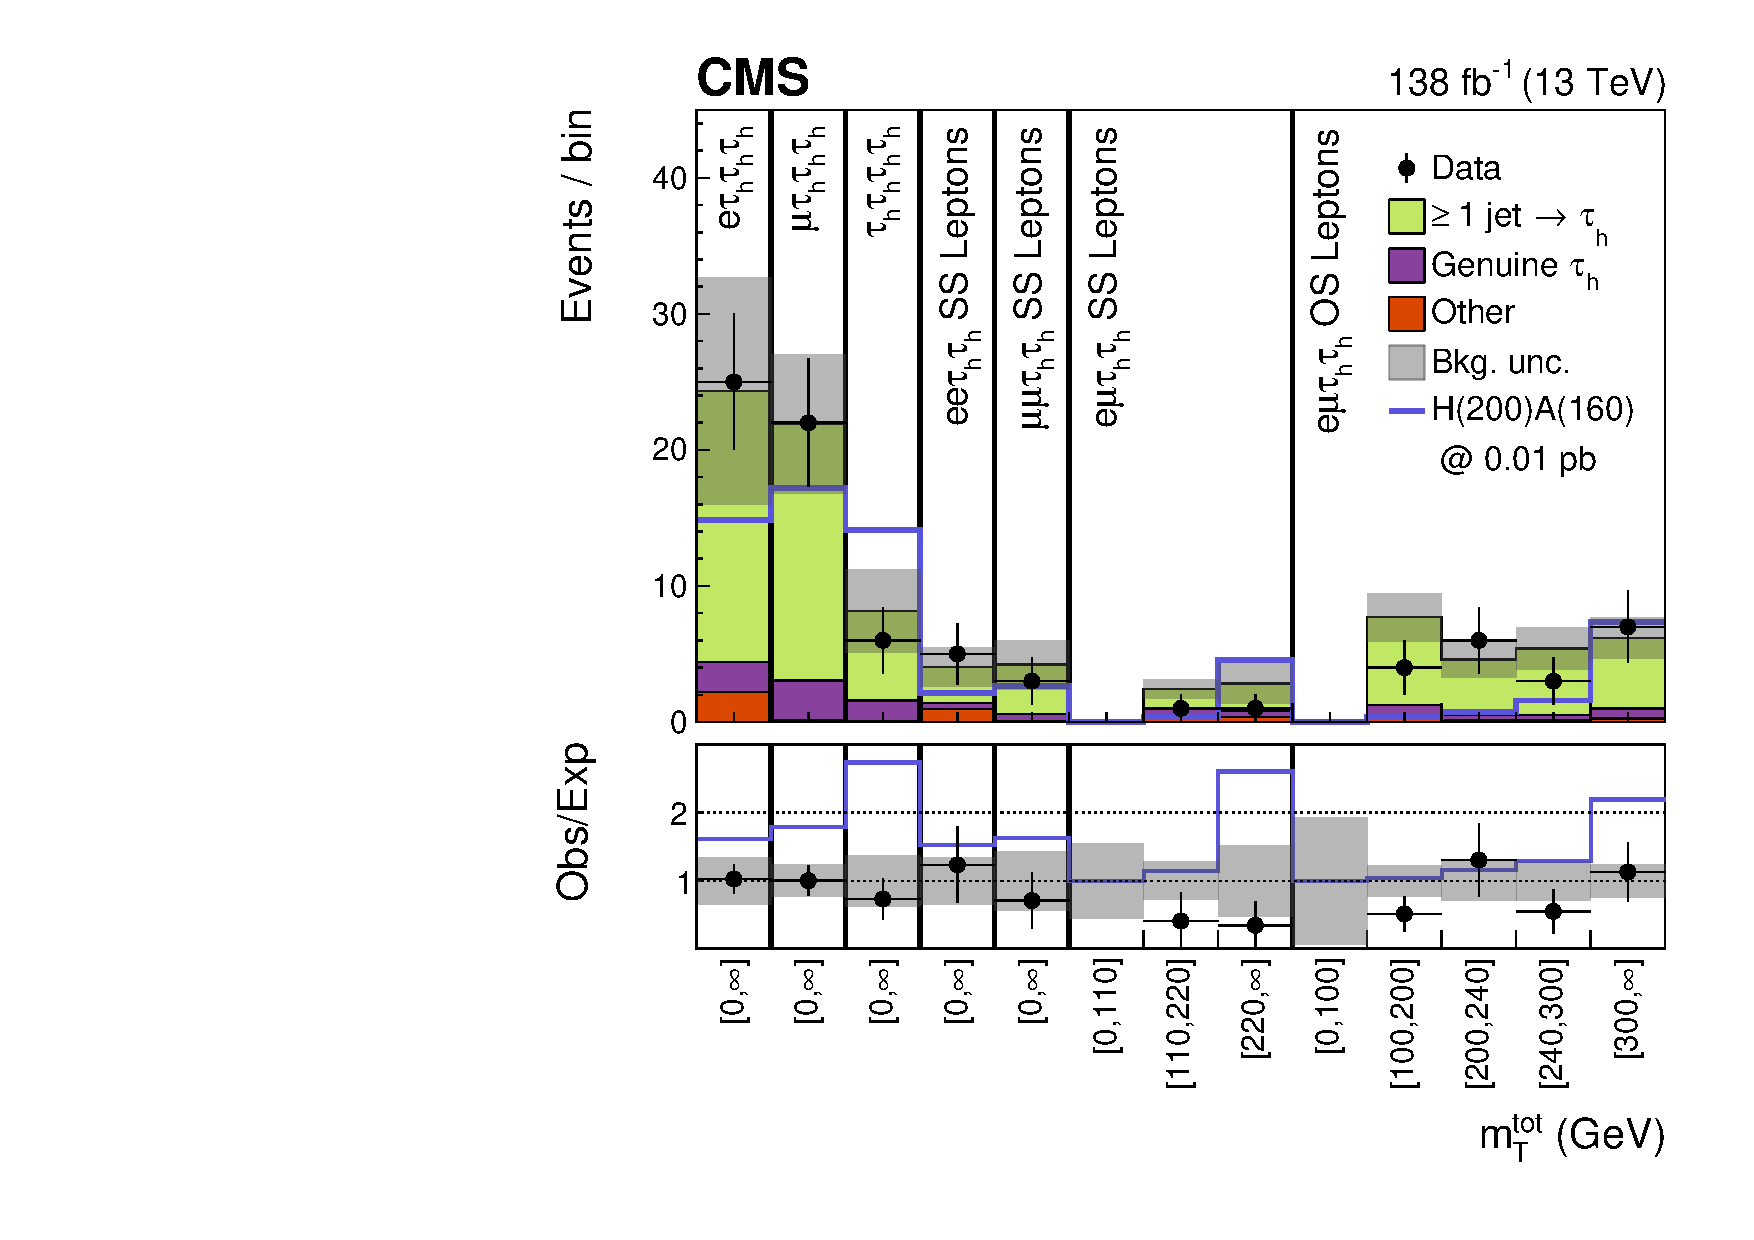
\includegraphics[width=\textwidth]{Figures/Chapter6/postfit_plots_combined_postfit_low_stat_paper.pdf}
            \caption{}
        \end{subfigure}
        \begin{subfigure}[b]{0.49\textwidth}
            \centering
            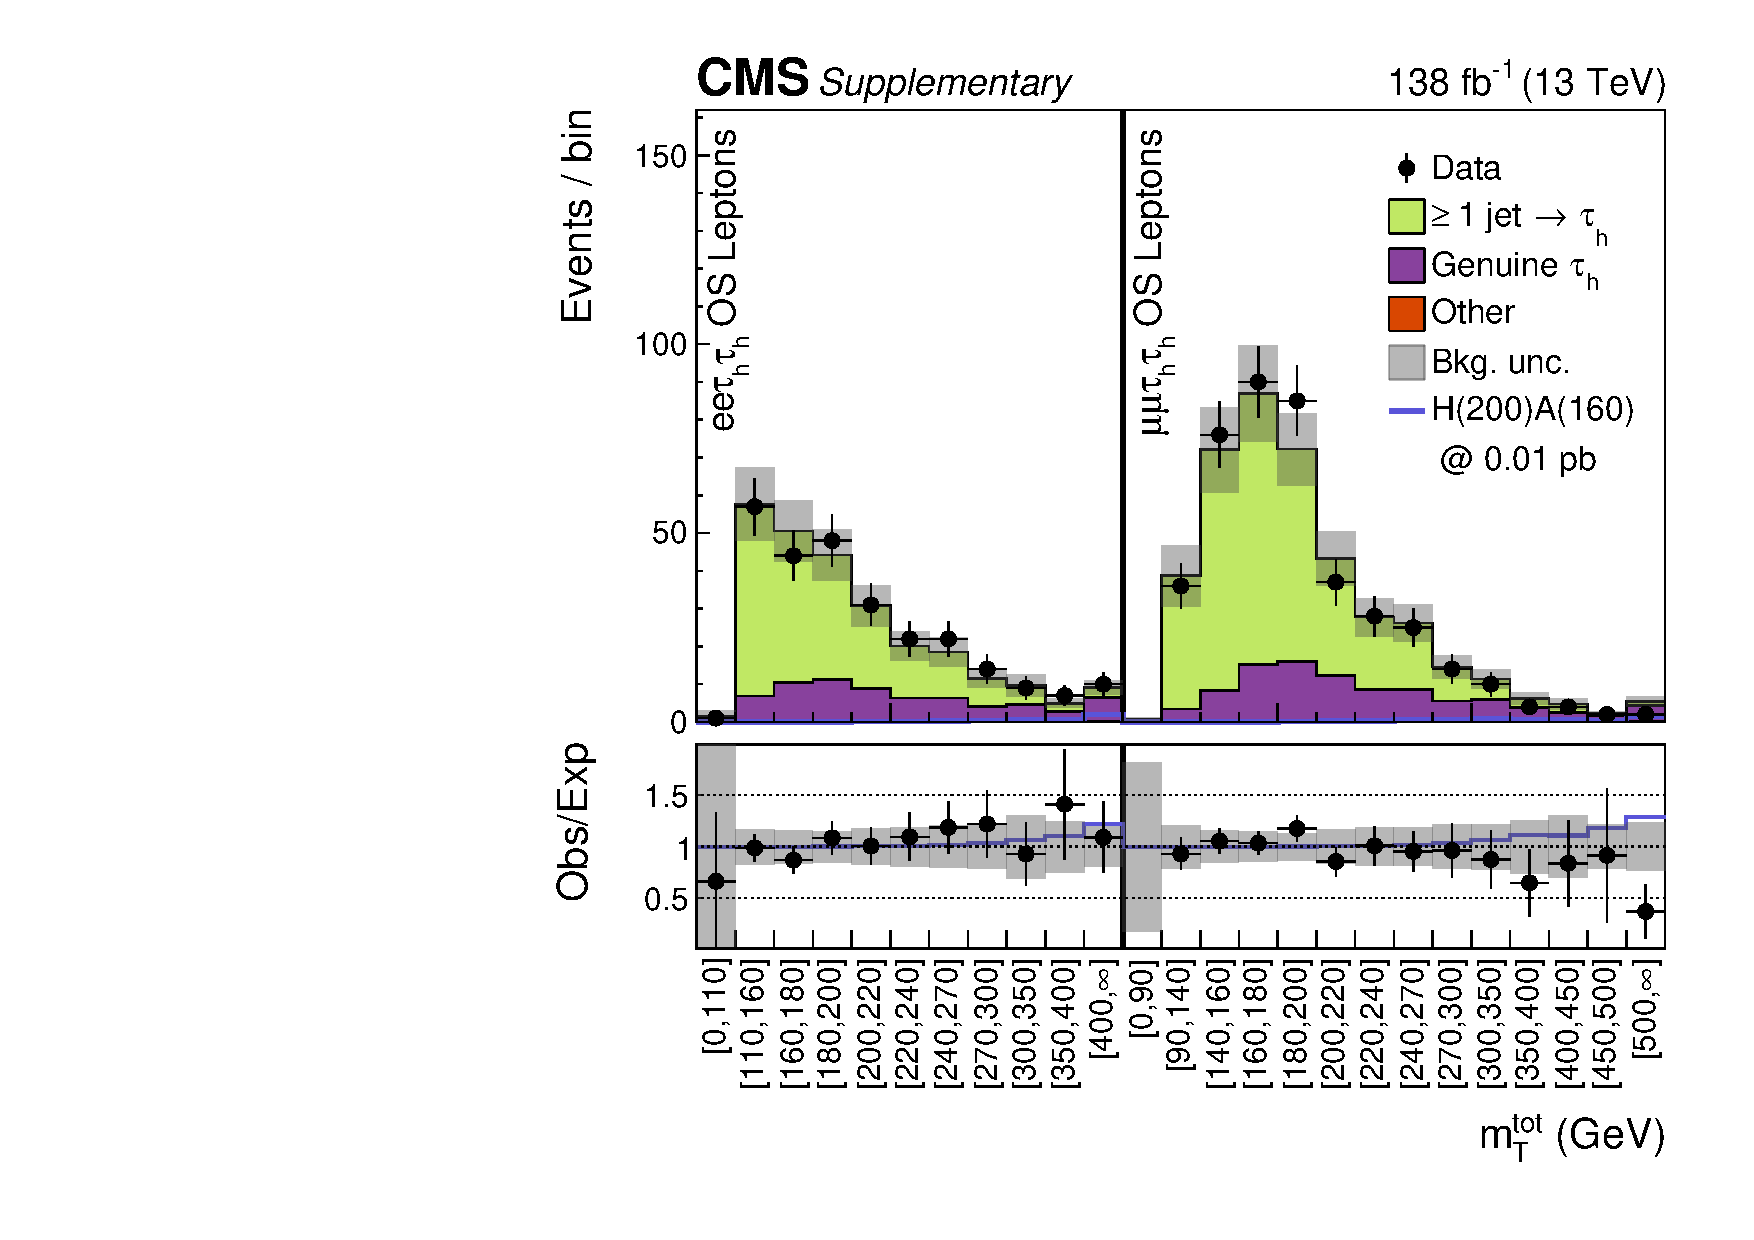
\includegraphics[width=\textwidth]{Figures/Chapter6/postfit_plots_combined_postfit_med_stat_paper.pdf}
            \caption{}
        \end{subfigure}
        \vspace{0.5cm}
        \begin{subfigure}[b]{0.49\textwidth}
            \centering
            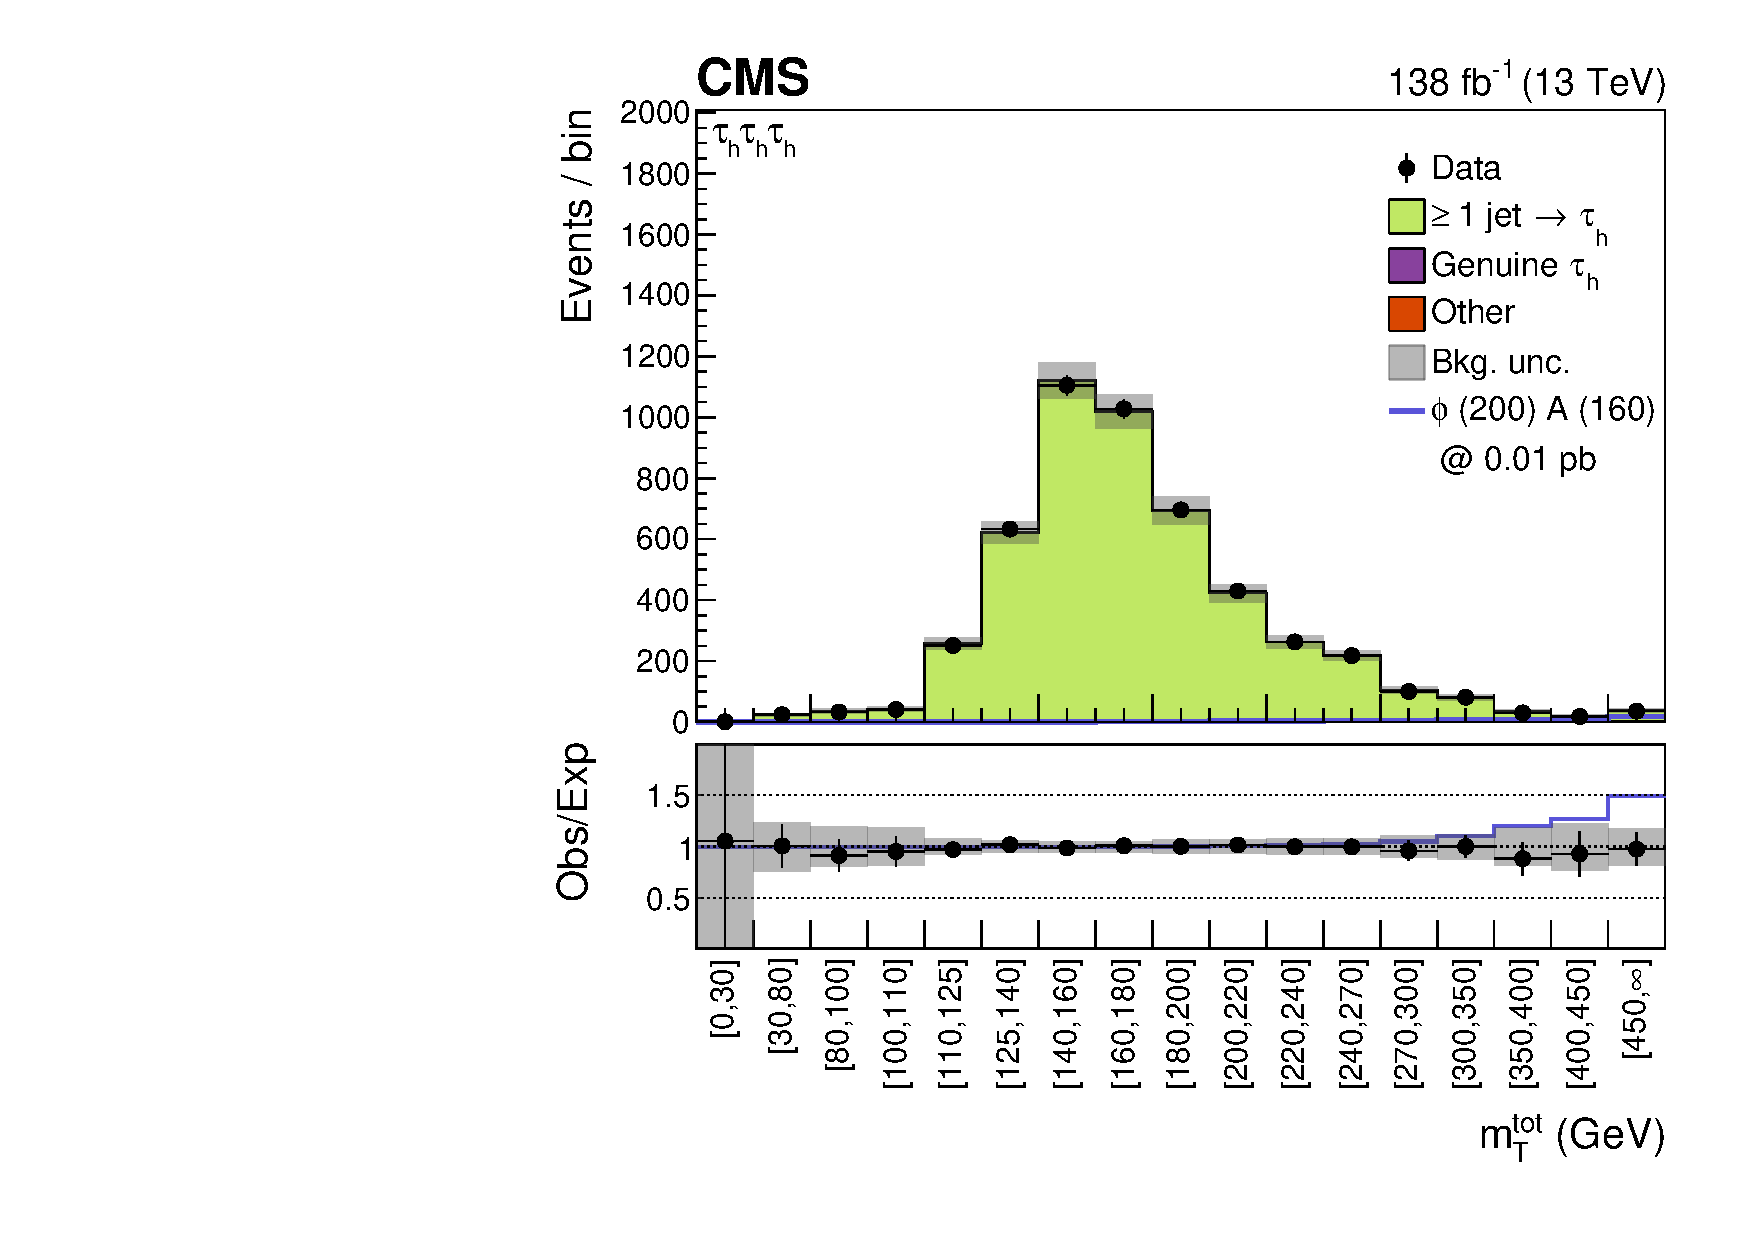
\includegraphics[width=\textwidth]{Figures/Chapter6/postfit_plots_combined_postfit_high_stat_paper.pdf}
            \caption{}
        \end{subfigure}

    \caption[Postfit $m_\mathrm{T}^\mathrm{tot}$ distributions in low-, medium-, and high-statistics categories.]{Postfit $m_\mathrm{T}^\mathrm{tot}$ distributions after the simultaneous background-only fit, shown for \textbf{(a)} low-statistics, \textbf{(b)} medium-statistics, and \textbf{(c)} high-statistics categories.}

    \label{Figure:Chapter6_PostfitDistributions}
\end{figure}

No significant excess is observed in any category or bin, and the combined results are consistent with the background-only hypothesis. Small local deficits in the number of observed events relative to the expectation are visible in certain bins, such as the $\PGt_e\PGt_\mu\PGt_h\PGt_h$ SS lepton category in the low-statistics group. To validate the dominant background contribution (jet$\to\PGt_h$) in these regions, an alternative approach was employed. The method estimates jet$\to\PGt_h$ contributions using simulated samples of processes (see Section~\ref{Section:Chapter6_Backgrounds}) with at least one jet reconstructed as a $\tau_{h}$, while the \ac{QCD} multijet background is obtained via a simple ABCD method in the $\sum q \neq 0$ region. The comparison shows predictions from this method to be in good agreement with those from the \ac{ML}-based $F_F$ approach.

\newpage
\subsection{Model-independent interpretation}

For the model‑independent interpretation, the signal yield is normalised to a reference cross section of $1\unit{pb}$. The parameter of interest is defined as the cross section for the $Z^* \to A\phi$ process multiplied by the branching fractions $\mathcal{B}(\phi \to \tau\tau)$ and $\mathcal{B}(A \to \tau\tau)$, under the assumption of a linear scaling $g(\mu) = \mu$. Observed upper limits at the 95\% CL are extracted for all mass hypotheses considered, following the procedure outlined in Section~\ref{Section:Chapter6_LimitExtraction}. The results, shown in Fig.~\ref{Figure:Chapter6_model_independent} as a two‑dimensional heatmap across the $(m_A, m_\phi)$ mass plane, span from $190\unit{fb}$ at $(m_A, m_\phi) = (40, 60)\GeV$ to $0.4\unit{fb}$ at $(m_A, m_\phi) = (600, 800)\GeV$.

\begin{figure}[!htbp]
    \centering        
    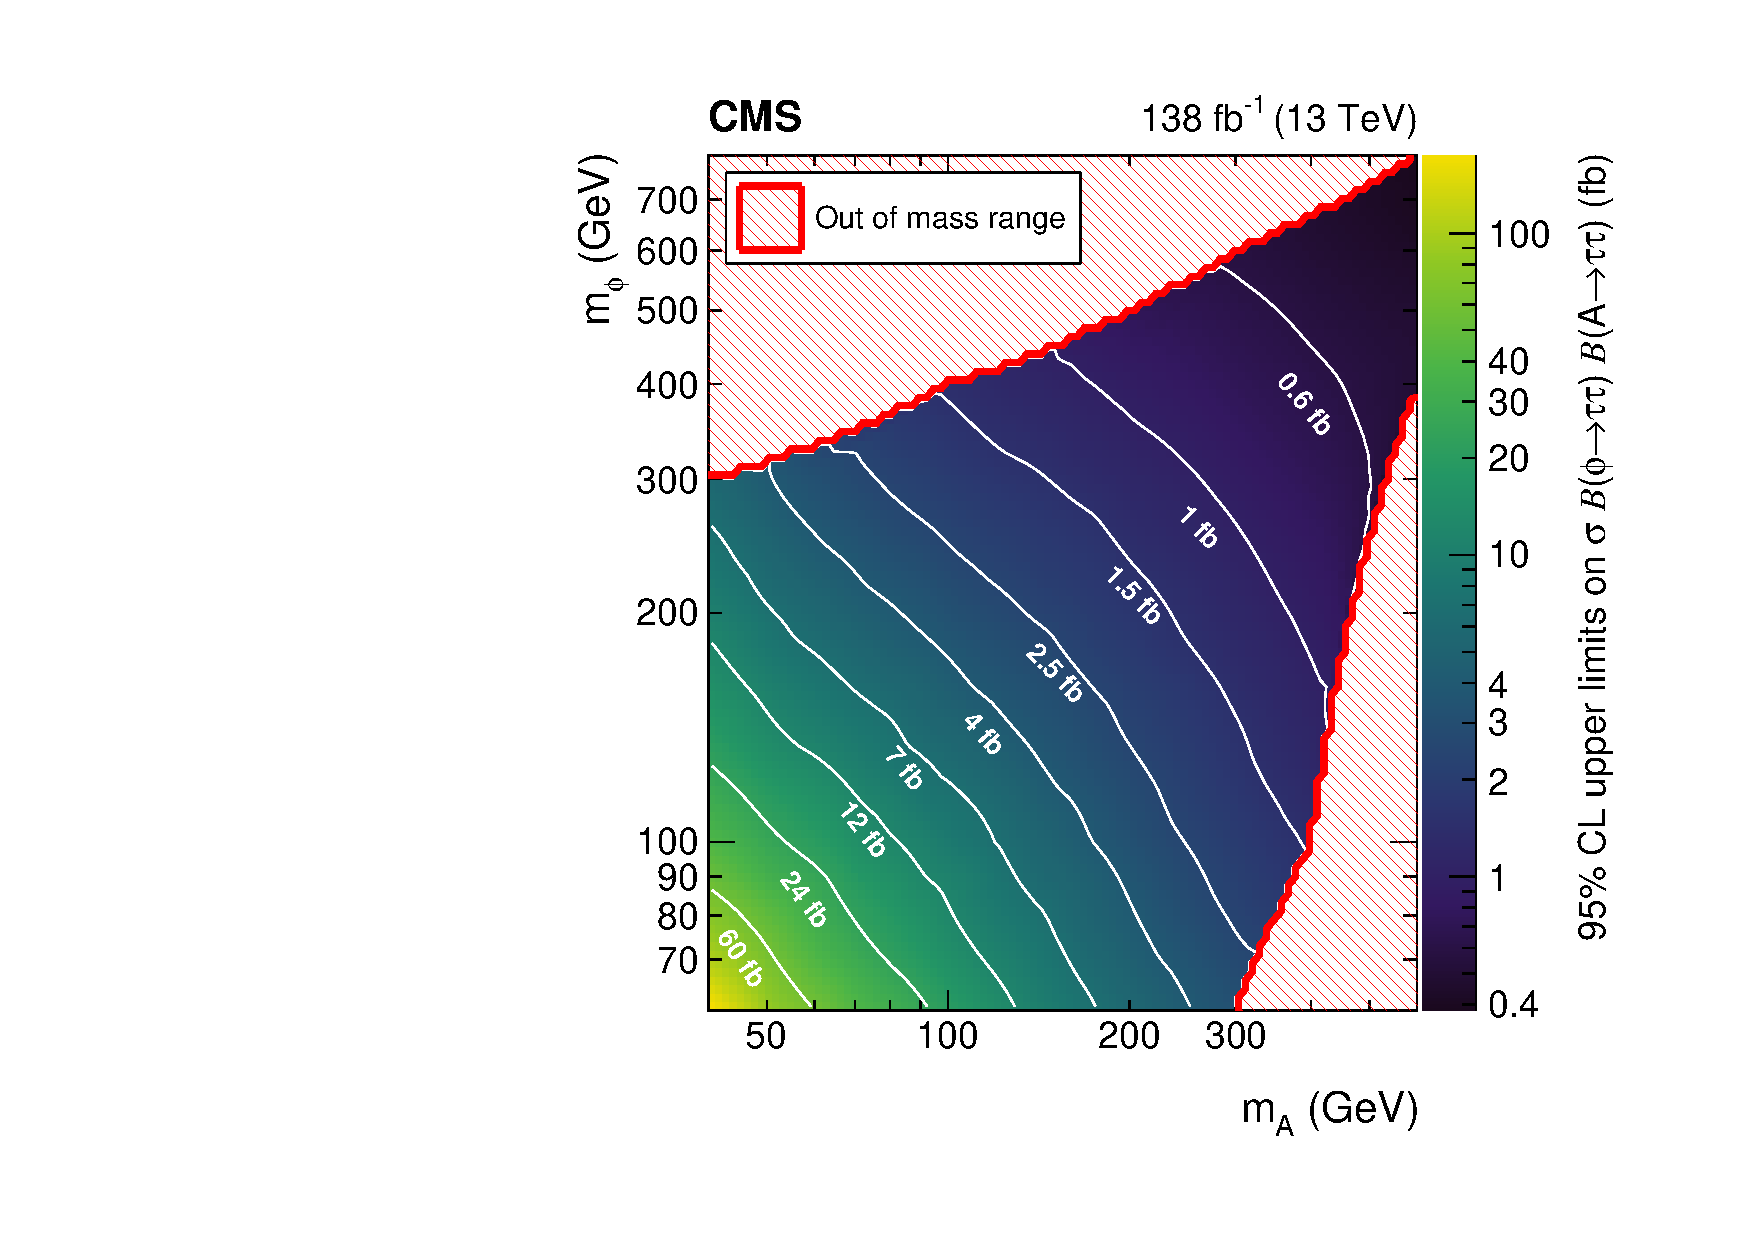
\includegraphics[width=0.7\textwidth]{Figures/Chapter6/mi_2d.pdf}
    \caption[Observed 95\% CL upper limits on $\sigma_\text{prod} \times \mathcal{B}(\phi\to\tau\tau)\times\mathcal{B}(A\to\tau\tau)$]{Observed 95\% CL upper limits on the product of the cross section ($\sigma_\text{prod}$) for the production of two \ac{BSM} Higgs bosons produced via an off-shell Z boson, and the branching fractions ($\mathcal{B}$) for their decay into $\PGt$ leptons. This is shown as a function of $m_A$ and $m_\phi$. No limits are set in the red hatched region.}
    \label{Figure:Chapter6_model_independent}
\end{figure}

A condensed view of the results for all 72 tested mass points is given in Fig.~\ref{Figure:Chapter6_model_independent_all}, where limits at higher $m_A$ values are scaled by increasing negative powers of ten for visual clarity.  Across the full mass range, the observed limits typically lie between the lower $1\sigma$ and $2\sigma$ expected bands. This is consistent with the small local deficits seen in Fig.~\ref{Figure:Chapter6_PostfitDistributions}, which strengthen the exclusion. All observed limits are well below the predicted cross sections shown in Fig.~\ref{Figure:Chapter6_ProductionXS}, demonstrating the strong sensitivity of the analysis to the Type-X \ac{2HDM} in the alignment scenario.

\begin{figure}[!htbp]
    \centering        
    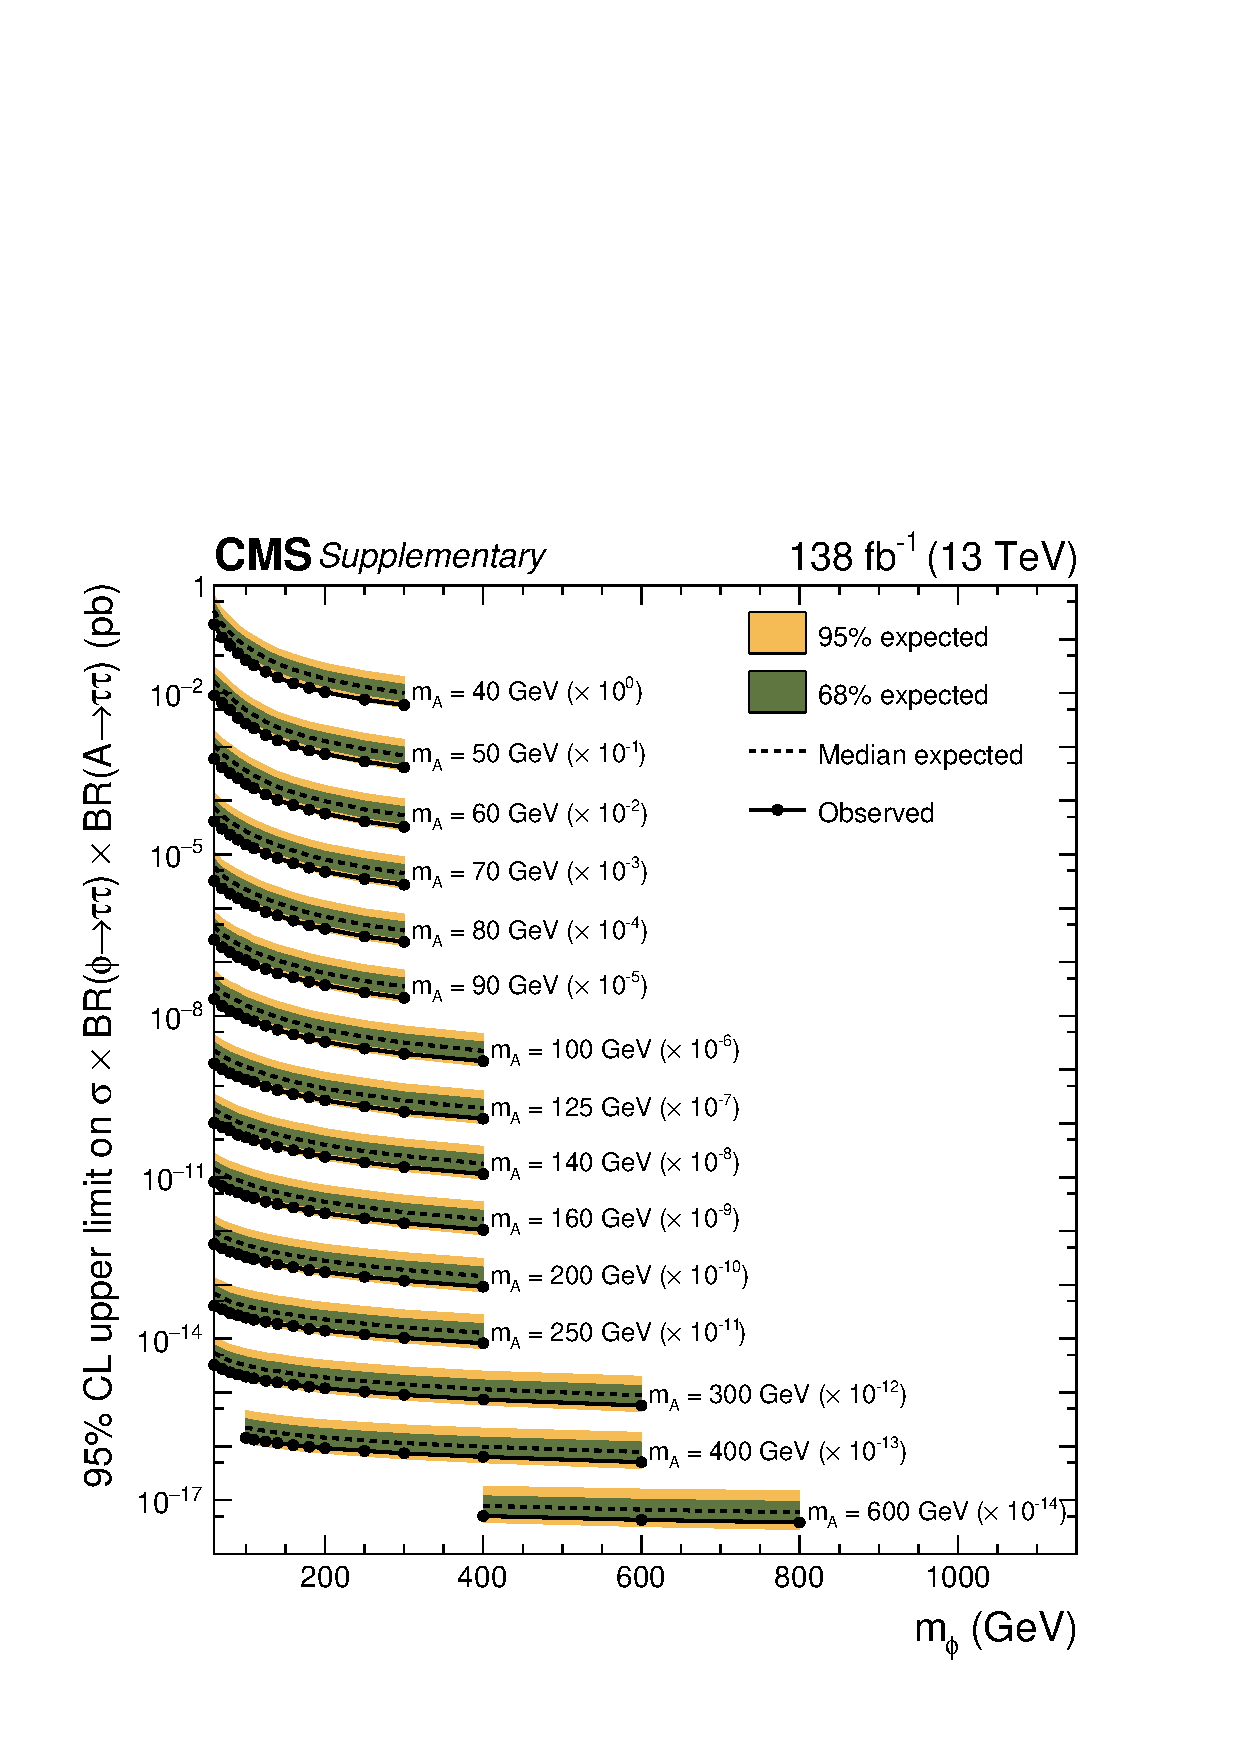
\includegraphics[width=0.7\textwidth]{Figures/Chapter6/model_independent_limit_all.pdf}
    \caption[Observed and expected 95\% CL upper limits on $\sigma_\text{prod} \times \mathcal{B}(\phi\to\tau\tau)\times\mathcal{B}(A\to\tau\tau)$]{Model-independent 95\% CL upper limits on the product of the production cross section ($\sigma_\text{prod}$) for two \ac{BSM} Higgs bosons, produced via an off-shell Z boson, and their branching fractions ($\mathcal{B}$) into $\PGt$ leptons, shown as a function of $m_A$ and $m_\phi$. Both expected and observed limits are presented, along with $\pm1\sigma$ and $\pm2\sigma$ uncertainty bands. For visual clarity, the limits at higher $m_A$ values are rescaled by increasing negative powers of ten, as indicated next to each curve.}
    \label{Figure:Chapter6_model_independent_all}
\end{figure}

\newpage
\subsection{Model-dependent interpretation}

For the model-dependent interpretation, the search results are translated into constraints on the Type-X \ac{2HDM} in the alignment scenario.  Each point in the $(m_A, \tan\beta)$ parameter space is tested by scaling the simulated signal samples to the predicted cross section times branching fractions for that point. A single rate parameter, defined as $g(\mu)=\mu$, is used, with $\mu=1$ corresponding to the Type-X \ac{2HDM} prediction and $\mu=0$ to the \ac{SM}. Figure~\ref{Figure:Chapter6_Model_Dependent} presents the 95\% CL exclusion contours in the $(m_A, \tan\beta)$ plane for two benchmark scenarios, $m_\phi = 100\GeV$ and $m_\phi = 200\GeV$. Furthermore, constraints from previous searches, obtained using \textsc{HiggsTools-1}~\cite{Bahl:2022igd}, are overlaid, together with the region favoured by the current muon anomalous magnetic moment measurement~\cite{TypeX_2HDM}.

\begin{figure}[!htbp]
        \centering
        % First row
        \begin{subfigure}[b]{0.6\textwidth}
            \centering
            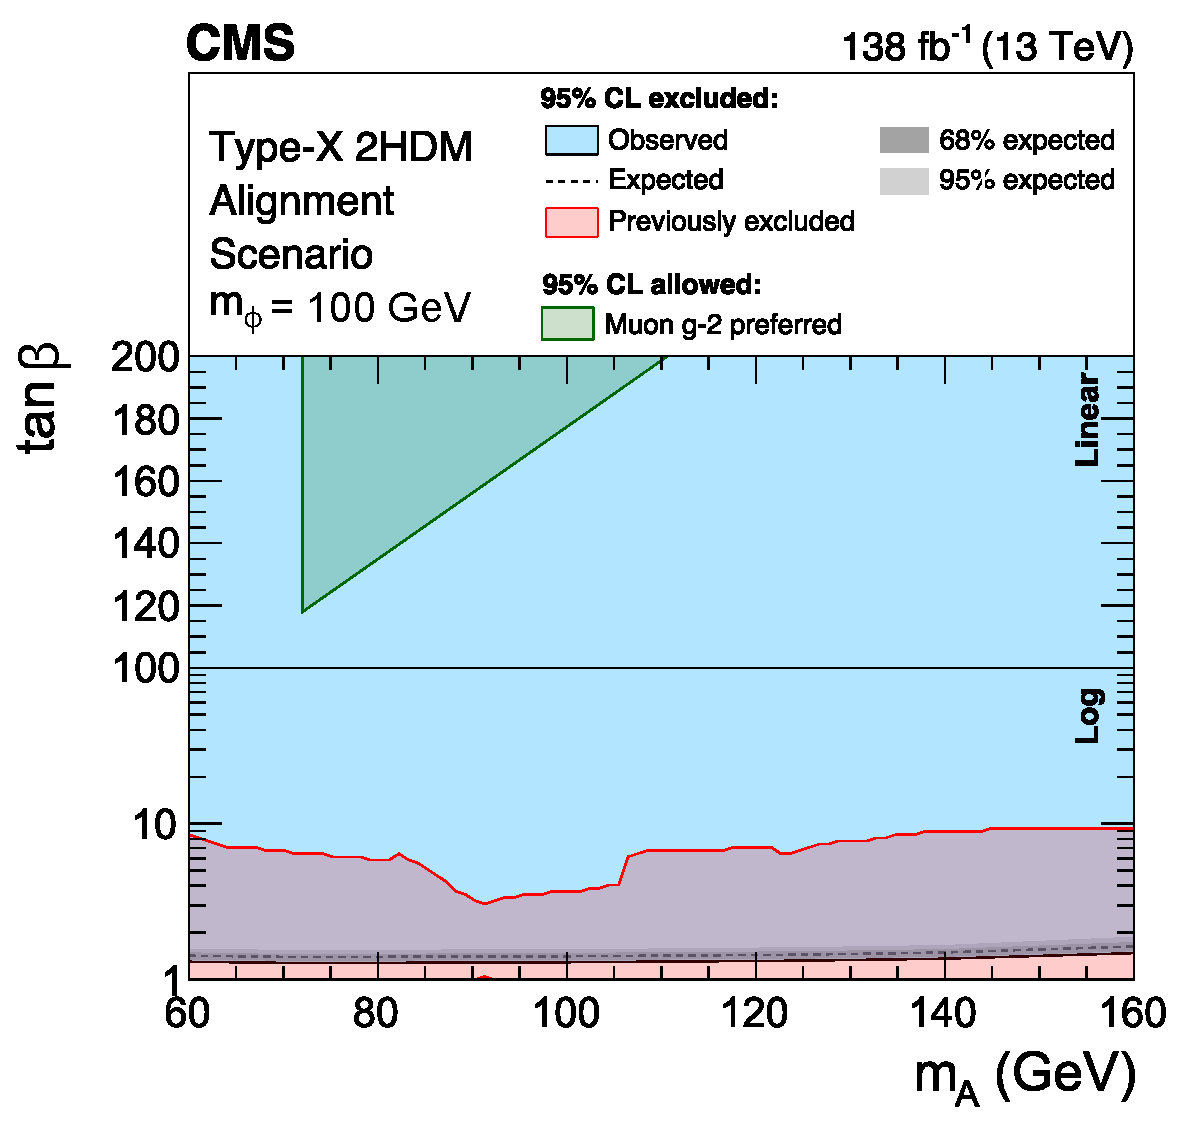
\includegraphics[width=\textwidth]{Figures/Chapter6/md_mphi100_hb_split_paper.pdf}
            \caption{}
        \end{subfigure}
        \begin{subfigure}[b]{0.6\textwidth}
            \centering
            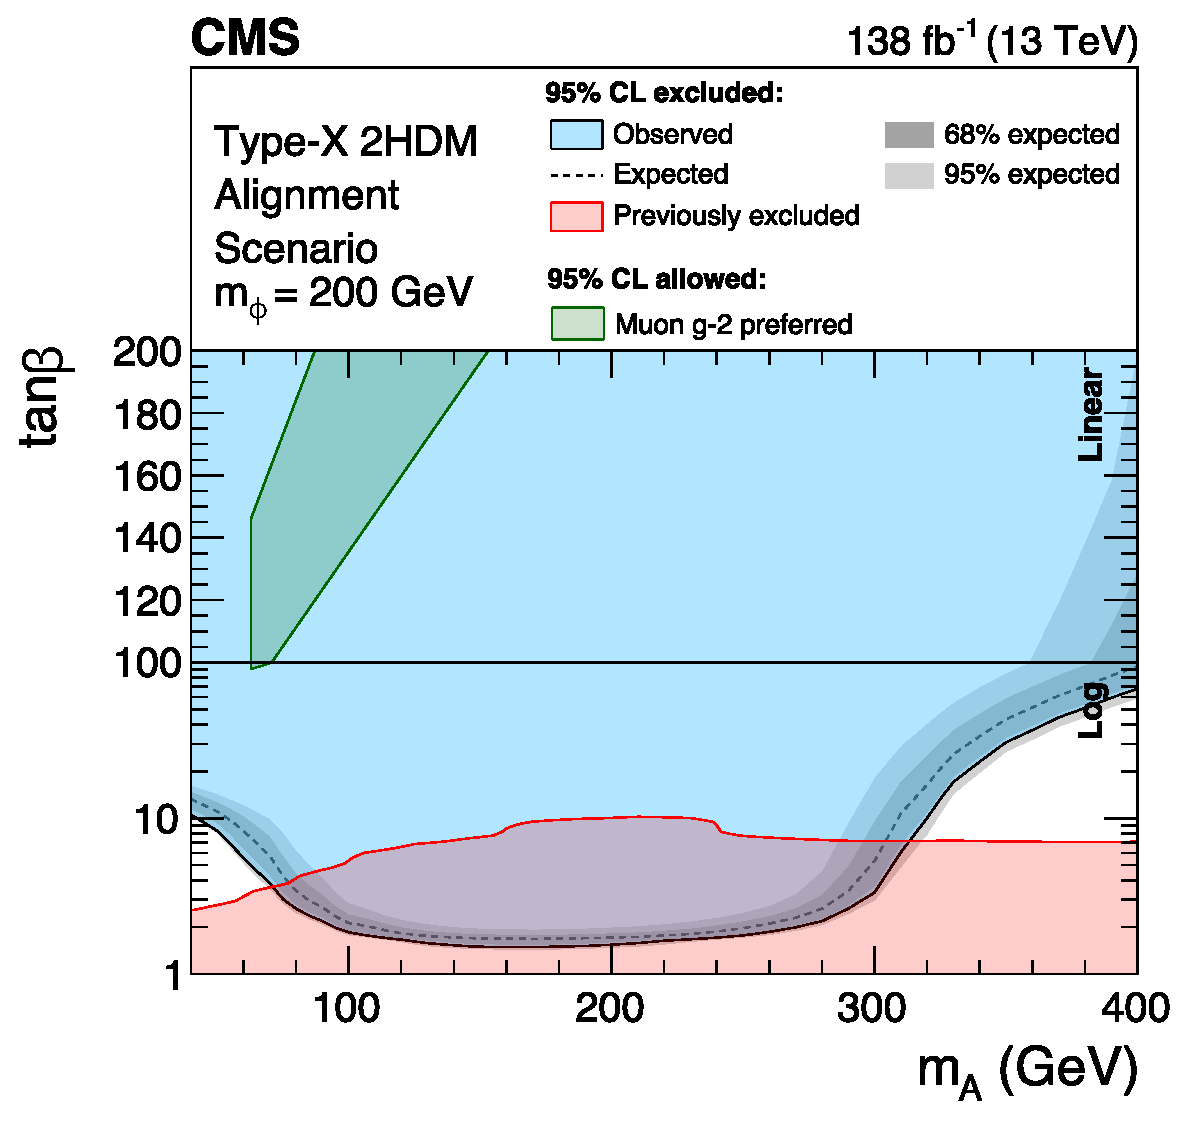
\includegraphics[width=\textwidth]{Figures/Chapter6/md_mphi200_hb_gm2_v3_paper.pdf}
            \caption{}
        \end{subfigure}

    \caption[95\% CL exclusion contours in the $(m_A, \tan\beta)$ plane for two $m_\phi$ benchmarks.]{Observed and expected 95\% confidence level exclusion contours in the $(m_A, \tan\beta)$ plane for the model-dependent interpretation, shown for benchmark masses \textbf{(a)} $m_\phi = 100\GeV$ and \textbf{(b)} $m_\phi = 200\GeV$. Constraints from previous searches, obtained using \textsc{HiggsTools-1}~\cite{Bahl:2022igd}, are overlaid, together with the parameter space favoured by the current muon anomalous magnetic moment measurement~\cite{TypeX_2HDM}.}
    \label{Figure:Chapter6_Model_Dependent}
\end{figure}

In the $m_\phi = 100\GeV$ scenario, the exclusion limit remains largely flat as a function of $m_A$, excluding values of $\tan\beta \gtrsim 2$. Below this threshold, the branching fractions of the $h$ and $A$ bosons to $\tau$ leptons drop sharply, with decays to $b\bar{b}$ becoming dominant, as discussed in Section~\ref{Section:Chapter6_production_xs_bf}. For $m_\phi = 200\GeV$, the exclusion is approximately constant in regions where both $m_A > m_\phi - m_{\PZ}$ and $m_\phi > m_A - m_{\PZ}$, reaching down to $\tan\beta \approx 1.5$. However, when the mass separation between $m_\phi$ and $m_A$ exceeds $m_{\PZ}$, the sensitivity degrades due to the opening of the $\PH \to \PZ A$ or $A \to \PZ \PH$ decay channels, which dominate the branching fractions in these regions (see Section~\ref{Section:Chapter6_production_xs_bf}).

A summary of the exclusion contours in the $m_A-m_\phi$ plane is shown in Fig.~\ref{Figure:Chapter6_model_dependent_2d}. This also shows the complete exclusion contours of the Type-X \ac{2HDM} alignment scenario from the union of the observed results and the limits obtained using $\textsc{HiggsTools-1}$~\cite{Bahl:2022igd}, as well as the allowed regions for an explanation of the muon anomalous magnetic moment~\cite{TypeX_2HDM}. Figure~\ref{Figure:Chapter6_model_dependent_2d} demonstrates the exclusion of this model as an explanation for the muon anomalous magnetic moment, as the allowed regions at high $\tan\beta$ in both the normal and inverted scenarios (green contours) are contained within the $\tanb > 15$ observed exclusion contour.
It also presents the complete exclusion of the Type-X \ac{2HDM} alignment scenario down a diagonal in the $m_A-m_\phi$ plane (red contour), with an approximate width of $100\GeV$, from the lowest mass point searched for at $m_A = 40\GeV$ and $m_\phi = 60\GeV$ to $m_\phi\approx m_A\approx360\GeV$.

\begin{figure}[!htbp]
  \centering
  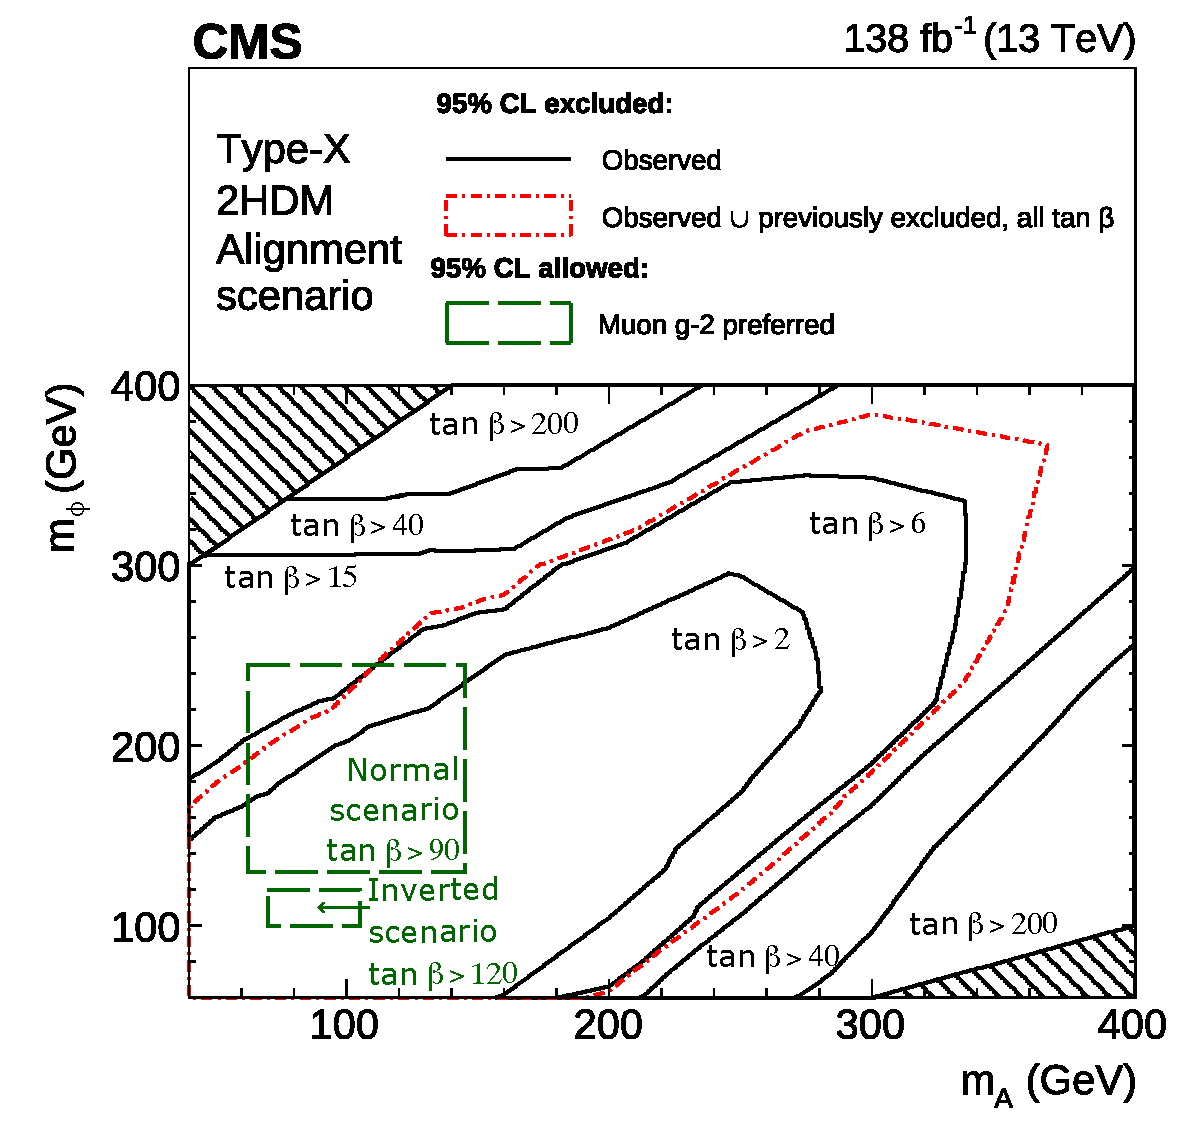
\includegraphics[width=0.6\textwidth]{Figures/Chapter6/md_2d_hb_gm2_contour.pdf}
  \caption[Summary of exclusion contours in the $m_A-m_\phi$ plane.]{
   Observed 95\% CL exclusions of the Type-X \ac{2HDM} alignment scenario in the $m_A$-$m_\phi$ plane are shown as black solid contours, with the $\tan\beta$ exclusion of each bounded region written on the plot.
   The complete exclusion of this model from the union of the observed limits and those obtained by $\textsc{HiggsTools-1}$~\cite{Bahl:2022igd} is enclosed by the red dot-dashed contour.
   The allowed regions accommodating the current measurement of the muon anomalous magnetic moment, as detailed in Ref.~\cite{TypeX_2HDM}, are shown as green dashed boxes, with the $\tan\beta$ allowed range written on the plot. Hatched regions indicate parameter space for which no exclusion limit is set.
  }
  \label{Figure:Chapter6_model_dependent_2d}
\end{figure}

In summary, a search has been performed for signatures of extended Higgs sectors in the four‑tau final state, targeting the process $Z^* \to \phi A \to \PGt^+\PGt^-\PGt^+\PGt^-$ in pp collisions at $\sqrt{s} = 13\TeV$ with the \ac{CMS} detector, using the full Run 2 dataset corresponding to an integrated luminosity of $138\unit{fb}^{-1}$. No significant excess above the \ac{SM} expectation is observed, and the results are interpreted as upper limits on the production cross section times branching fraction, which range from $\mathcal{O}(0.4\unit{fb})$ at high $(m_A, m_\phi)$ to $\mathcal{O}(190\unit{fb})$ at low masses. These constraints exclude a substantial fraction of the parameter space of the Type‑X \ac{2HDM}, including the region compatible with an explanation of the muon anomalous magnetic moment as proposed in Ref.~\cite{TypeX_2HDM}.










